\documentclass[a4paper,11pt,openright,numbers=noenddot]{scrreprt}

\usepackage[utf8]{inputenc} % Einstellung der Eingabekodierung
\usepackage[ngerman]{babel} % Deutsche Trennmuster
\usepackage{newpxtext} % Schriftart Palatino
\usepackage{newpxmath} % passende Mathe-Schrift
\usepackage[T1]{fontenc} % Einstellung Schriftkodierung
\usepackage{amsmath} % Mathematik-Erweiterungen
\usepackage{microtype} % Verbesserte Mikrotypographie
\usepackage{csquotes} % Kontextabhängige Anführungszeichen
\usepackage{calc} % Berechnung von TeX-Maßen
\usepackage[%
  inner=25mm,%
  outer=35mm,%
  top=25mm,%
  bottom=30mm,%
  includeheadfoot,%
  headheight=14pt,%
  marginparwidth=25mm%
]{geometry} % Anpassung Satzspiegel
\usepackage{array} % Tabellen-Erweiterung
\usepackage{graphicx} % Einbindung von Grafiken
\usepackage{float} % Anpassung von Gleitumgebungen
\usepackage{acro} % Abkürzungen
\acsetup{make-links = true}
\usepackage{listings} % Codeblöcke
\usepackage{pgfplots} % Plots
\pgfplotsset{compat=1.18}
\usepackage{pgfplotstable} % CSV für Plots importieren
\usepgfplotslibrary{statistics} % Boxplots
\usepackage{csvsimple} % CSV für Tabellen importieren
\usepackage{booktabs} % Tabellenlinien
\usepackage{pdfpages} % Einbindung von externen PDFs
\usepackage{letltxmacro} % redefining commands with optional arguments
\usepackage{xcolor} % for colorlet command
\usepackage{svg} % includesvg
\usepackage{subcaption} % subfigures
\usepackage{tikz}
\usetikzlibrary{shapes, calc, positioning}
\usepackage{environ} % scale tikz picture to width
% \usepackage{amssymb} % blacktriangleright

\usepackage[style=apa,backend=biber,natbib]{biblatex}

% auf Einbindungsreihenfolge achten
\usepackage{hyperref}


% können nach Fertigstellung gelöscht werden
\usepackage{todonotes} % TODO-Anmerkungen
\usepackage{marginnote}
\let\marginpar\marginnote
\usepackage{lipsum} % Blindtexte
\usepackage{blindtext} % Blindtexte
\usepackage{layout} % Darstellung des Satzspiegels

\floatplacement{figure}{htb}
\floatplacement{table}{htb}
   % Anpassungen für Gleitumgebungen
% Umgebung für das Deckblatt
\newenvironment{tuctitlepage}
{
  \cleardoublepage
  \titlepage
  \center
}
{
  \endcenter
  \endtitlepage
}


% Professur, Institut, ...
\newenvironment{tuctitleorgunit}{\center}{\endcenter}


% Logo
\newcommand{\tuctitlelogoname}{tuc/tuc_green_margin}

\newcommand{\tuctitlelogo}[1][0.6\linewidth]
{%
  \begin{center}%
    \includegraphics[width=#1]{\tuctitlelogoname}%
  \end{center}%
}


% Block mit kleiner Überschrift.
\newenvironment{tuctitleblock}[2][\medskipamount]
{\center\vspace*{#1}{#2\par}\vspace*{#1}}
{\par\endcenter}


% Art der Arbeit
\newcommand{\tuctitlethesistype}[1]
{\begin{center}{\huge\bfseries#1}\par\end{center}}


% Angestrebter Abschluss
\newcommand{\tuctitledegreephrase}{zur Erlangung des akademischen Grades}
\newcommand{\tuctitledegreeline}[1]
{{\LARGE #1}\par}
\newcommand{\tuctitledegree}[2][\medskipamount]
{\begin{tuctitleblock}[#1]{\tuctitledegreephrase}%
    \tuctitledegreeline{#2}%
  \end{tuctitleblock}}


% Autor
\newcommand{\tuctitleauthorphrase}{vorgelegt von}
\newcommand{\tuctitleauthorline}[1]
{{\Large #1}\par}
\newcommand{\tuctitleauthor}[2][\medskipamount]
{\begin{tuctitleblock}[#1]{\tuctitleauthorphrase}%
    \tuctitleauthorline{#2}%
  \end{tuctitleblock}}


% Lehrveranstaltung
\newcommand{\tuctitlecoursephrase}{zur Lehrveranstaltung}
\newcommand{\tuctitlecourseline}[1]
{{\LARGE #1}\par}
\newcommand{\tuctitlecourse}[2][\medskipamount]
{\begin{tuctitleblock}[#1]{\tuctitlecoursephrase}%
    \tuctitlecourseline{#2}%
  \end{tuctitleblock}}


% Semester
\newcommand{\tuctitletermphrase}{im}
\newcommand{\tuctitletermline}[1]
{{\Large #1}\par}
\newcommand{\tuctitleterm}[2][\medskipamount]
{\begin{tuctitleblock}[#1]{\tuctitletermphrase}%
    \tuctitletermline{#2}%
  \end{tuctitleblock}}


% Thema der Arbeit
\newenvironment{tuctitletopic}
{\center\LARGE\medskip\begingroup}
{\par\endgroup\medskip\endcenter}


%
% Deckblatttabellen ohne Einzug
%
% #1 -> Formatierung der linken Spalte
% #2 -> Anzahl rechter Spalten
%
\newenvironment{tuctitletable}[2][]
{\center\tabular{>{#1}r*{#2}{l}}}
{\endtabular\endcenter}


%
% Deckblatttabellen mit Einzug
%
% #1 -> Formatierung der linken Spalte
% #2 -> Anzahl rechter Spalten
% #3 -> Breite der linken Spalte
%
\newenvironment{tuctitletableindent}[3][]
{\flushleft\tabular{@{}>{\raggedleft#1}p{#3-\tabcolsep}*{#2}{l}}}%
{\endtabular\endflushleft}


% Datum, Ort
\newcommand{\tuctitleplacedate}[1]
{\center\medskip#1\par\endcenter}
 % Formatvorlage für das Deckblatt
\newenvironment{tucsimplesection}[2][\bigskipamount]
{
  \par\centerline{\textbf{\Large #2}}\par
  \vspace*{#1}
}
{}
 % Einfache Überschriften für Aufgabenstellung usw.
\newenvironment{tucerklaerung}[1][Selbstständigkeitserklärung]
{
  \pagestyle{empty}
  \thispagestyle{empty}
  \newcommand{\tucsignature}[2][5cm]%
  {
    \par
    \begin{flushright}
      \begin{minipage}{##1}
        \footnotesize
        \vbox{\hbox to \hsize{\rule{0pt}{7ex}\dotfill}\hbox{\hspace{1em}##2}}
      \end{minipage}
    \end{flushright}
  }
  \tucsimplesection{#1}
}
{
  \endtucsimplesection
}
 % Formatvorlage für die Selbstständigkeitserklärung
% https://tex.stackexchange.com/a/302313
\makeatletter
\newcommand{\newstarcommand}[1]{%
  \DeclareRobustCommand#1{%
    \@ifstar{\csname s\string#1\endcsname}{\csname n\string#1\endcsname}%
  }%
  \edef\meta@def@name{\string#1}%
  \meta@def
}
\newcommand\meta@def[3][0]{%
  \expandafter\newcommand\csname n\meta@def@name\endcsname[#1]{#2}%
  \expandafter\newcommand\csname s\meta@def@name\endcsname[#1]{#3}%
}
\makeatother

% todo footnotes
% \newcounter{todocounter}
% \setcounter{todocounter}{100}
% \newcommand{\todo}[1]{\refstepcounter{todocounter}\textcolor{red}{\footnote[\thetodocounter]{\textcolor{gray}{TODO: #1}}}}

% inline box notes
\newcommand{\boxnote}[1]{%
  \bigbreak
  \begin{center}
    \noindent\fbox{\parbox{0.85\textwidth}{#1}}
  \end{center}
  \bigbreak
}
 % util commands
\defbibfilter{articles}{
  type=article or
  type=inproceedings or
  type=report
}

\defbibfilter{books}{
  type=book or
  type=inbook or
  type=incollection
}

\defbibfilter{software}{
  type=software
}

\defbibfilter{other}{
  type=misc or
  type=thesis or
  type=online or
  type=legislation
}

\DefineBibliographyStrings{ngerman}{
  nodate = {{}o\adddot \space D\adddot},
  mathesis = {Masterarbeit}
}

\makeatletter
% cite the alias like this: OGC (2016) or Open Geospatial Consortium (OGC) (2016)
\DeclareCiteCommand{\textcitealias}
{\usebibmacro{prenote}}
{\usebibmacro{citeindex}%
  \printtext[bibhyperref]{\@citealias{\thefield{entrykey}} (\citeyear{\thefield{entrykey}})}}
{\multicitedelim}
{\usebibmacro{postnote}}

% cite the alias like this: (OGC, 2016) or (Open Geospatial Consortium (OGC), (2016))
\DeclareCiteCommand{\parencitealias}[\mkbibparens]
{\usebibmacro{prenote}}
{\usebibmacro{citeindex}%
  \printtext[bibhyperref]{\@citealias{\thefield{entrykey}}, \citeyear{\thefield{entrykey}}}}
{\multicitedelim}
{\usebibmacro{postnote}}

% cite the alias with a forced short form like this: OGC (2016)
\DeclareCiteCommand{\textcitealiass}
{\usebibmacro{prenote}}
{\usebibmacro{citeindex}%
  \printtext[bibhyperref]{\@citealias{\thefield{entrykey}S} (\citeyear{\thefield{entrykey}})}}
{\multicitedelim}
{\usebibmacro{postnote}}

% cite the alias with a forced short form like this: (OGC, 2016)
\DeclareCiteCommand{\parencitealiass}[\mkbibparens]
{\usebibmacro{prenote}}
{\usebibmacro{citeindex}%
  \printtext[bibhyperref]{\@citealias{\thefield{entrykey}S}, \citeyear{\thefield{entrykey}}}}
{\multicitedelim}
{\usebibmacro{postnote}}
\makeatother

\defcitealias{ogcOGC}{\ac{OGC}}
\defcitealias{ogcCatalogue2016}{\ac{OGC}}
\defcitealias{ogcFiltering}{\ac{OGC}}
\defcitealias{ogcFilteringS}{\acs*{OGC}}
\defcitealias{ogcOGCAPI12022}{\ac{OGC}}
\defcitealias{ogcOGCAPI22022}{\ac{OGC}}
\defcitealias{ogcOGCAPI4}{\ac{OGC}}
\defcitealias{ISO924111}{ISO/TC 159 Ergonomics SC 4}
\defcitealias{unisd2021}{UNIS-D}
\defcitealias{bootstrapIcons}{Bootstrap Icons}
\defcitealias{scratchfoundationScratch}{Scratch}
\defcitealias{monigSnap}{\textit{Snap!}}
 % bib utils
\renewcommand{\lstlistingname}{Quelltext}
\renewcommand{\lstlistlistingname}{Quelltextverzeichnis\todo{Heißt das so?}}

\makeatletter
\let\orig@lstnumber=\thelstnumber

\newcommand\lstsetnumber[1]{\gdef\thelstnumber{#1}}
\newcommand\lstresetnumber{\global\let\thelstnumber=\orig@lstnumber}
\makeatother

\lstset{numbers=left}

\colorlet{punct}{red!60!black}
\definecolor{background}{HTML}{EEEEEE}
\definecolor{delim}{RGB}{20,105,176}
\colorlet{numb}{magenta!60!black}

\lstdefinelanguage{json}{
  basicstyle=\normalfont\ttfamily,
  numbers=left,
  numberstyle=\scriptsize,
  stepnumber=1,
  numbersep=8pt,
  showstringspaces=false,
  breaklines=true,
  frame=lines,
  backgroundcolor=\color{background},
  literate=
   *{:}{{{\color{punct}{:}}}}{1}
    {,}{{{\color{punct}{,}}}}{1}
    {\{}{{{\color{delim}{\{}}}}{1}
    {\}}{{{\color{delim}{\}}}}}{1}
    {[}{{{\color{delim}{[}}}}{1}
    {]}{{{\color{delim}{]}}}}{1},
}

\lstdefinelanguage{bnf}{
  basicstyle=\normalfont\ttfamily,
  numbers=left,
  numberstyle=\scriptsize,
  stepnumber=1,
  numbersep=8pt,
  showstringspaces=false,
  breaklines=true,
  frame=lines,
  backgroundcolor=\color{background},
  literate=
   *{=}{{{\color{punct}{=}}}}{1}
    {|}{{{\color{punct}{|}}}}{1}
    {;}{{{\color{punct}{;}}}}{1}
    {\{}{{{\color{delim}{\{}}}}{1}
    {\}}{{{\color{delim}{\}}}}}{1}
    {[}{{{\color{delim}{[}}}}{1}
    {]}{{{\color{delim}{]}}}}{1},
}
 % listings setup
\definecolor{plot1}{HTML}{4F81BD}
\definecolor{plot2}{HTML}{C0504D}
\definecolor{plot3}{HTML}{9BBB59}
\definecolor{plot4}{HTML}{9B0B59}
 % colors

%\makeglossaries
%\newacronym{asq}{ASQ}{After Scenario Questionnaire}
%\newacronym{csuq}{CSUQ}{Computer System Usability Questionnaire}
%\newacronym{cql}{CQL}{Common Query Language}
%\newacronym{pssuq}{PSSUQ}{Post-Study System Usability Questionnaire}
%\newacronym{cta}{CTA}{Concurrent Think-Aloud-Protokoll}
%\newacronym{nasa-tlx}{NASA-TLX}{NASA Task Load Index}
%\newacronym{nps}{NPS}{Net Promoter Score}
%\newacronym{rta}{RTA}{Retrospective Think-Aloud-Protokoll}
%\newacronym{seq}{SEQ}{Single Ease Question}
%\newacronym{smeq}{SMEQ}{Subjective Mental Effort Questionnaire}
%\newacronym{sus}{SUS}{System Usability Scale}
%\newacronym{ta}{TA}{Think-Aloud-Protokoll}
%\newacronym{ume}{UME}{Usability Magnitude Estimation}
\DeclareAcronym{asq}{short=ASQ,long=After Scenario Questionnaire}
\DeclareAcronym{csuq}{short=CSUQ,long=Computer System Usability Questionnaire}
\DeclareAcronym{cql}{short=CQL,long=Common Query Language}
\DeclareAcronym{pssuq}{short=PSSUQ,long=Post-Study System Usability Questionnaire}
\DeclareAcronym{cta}{short=CTA,long=Concurrent Think-Aloud-Protokoll}
\DeclareAcronym{nasa-tlx}{short=NASA-TLX,long=NASA Task Load Index}
\DeclareAcronym{nps}{short=NPS,long=Net Promoter Score}
\DeclareAcronym{rta}{short=RTA,long=Retrospective Think-Aloud-Protokoll}
\DeclareAcronym{seq}{short=SEQ,long=Single Ease Question}
\DeclareAcronym{smeq}{short=SMEQ,long=Subjective Mental Effort Questionnaire}
\DeclareAcronym{sus}{short=SUS,long=System Usability Scale}
\DeclareAcronym{ta}{short=TA,long=Think-Aloud-Protokoll}
\DeclareAcronym{ume}{short=UME,long=Usability Magnitude Estimation}
 % acronyms
\newcommand{\organization}{
    Technische Universität Chemnitz \\
    Fakultät Informatik \\
    Professur Medieninformatik \\
}
\newcommand{\thesistype}{Bachelorarbeit}
\newcommand{\degree}{Bachelor of Science}
\newcommand{\theauthor}{Joshua Jeschek}
\newcommand{\thetitle}{Blockbasierte Daten-Konvertierung}
\newcommand{\thesubtitle}{Einschätzung der empfundenen Produktivitätssteigerung im Umgang mit Umweltdaten}
\newcommand{\erstpruefer}{Dr. Thomas Wilhelm-Stein}
\newcommand{\zweitpruefer}{Dr. Werner Koch}
\newcommand{\place}{Chemnitz}
\date{\today\todo{Einreichung}}

\author{\theauthor}
\title{\thetitle}
\subtitle{\thesubtitle}
 % acronyms

\addbibresource{bibliography.bib}

\MakeOuterQuote{"} % könnte zu Problemen führen

\raggedbottom

\begin{document}
\pagenumbering{roman}
\makeatletter
\begin{tuctitlepage}
  \begin{tuctitleorgunit}
    \organization
  \end{tuctitleorgunit}

  \tuctitlelogo

  \tuctitlethesistype{\thesistype}
  \bigskip
  \tuctitledegree{\degree}
  \bigskip
  \tuctitleauthor{\@author}

  \vspace*{0pt plus 2fill}
  \begin{tuctitletopic}
    \@title \\
    \large{\@subtitle}
  \end{tuctitletopic}
  \vspace*{0pt plus 2fill}

  \begin{tuctitletable}[\bfseries]{1}
    Erstprüfer:  & \erstpruefer \\
    Zweitprüfer: & \zweitpruefer \\
  \end{tuctitletable}

  \vspace*{0pt plus 1fill}

  \tuctitleplacedate{\place, \@date}
\end{tuctitlepage}
\makeatother

\cleardoublepage
\vspace*{0pt plus 1fill}
\begin{tucsimplesection}{Abstract}
  \blindtext\todo{anpassen}
\end{tucsimplesection}
\vspace*{0pt plus 2.5fill}


\cleardoublepage
\currentpdfbookmark{Inhaltsverzeichnis}{name}
\tableofcontents

\cleardoublepage
\phantomsection
\addcontentsline{toc}{chapter}{\listfigurename}
\listoffigures

\cleardoublepage
\phantomsection
\addcontentsline{toc}{chapter}{\listtablename}
\listoftables

\cleardoublepage
\phantomsection
\addcontentsline{toc}{chapter}{\lstlistlistingname}
\lstlistoflistings

\cleardoublepage
\phantomsection
\addcontentsline{toc}{chapter}{Abkürzungen}
\printacronyms


\cleardoublepage
\pagenumbering{arabic}

\chapter{Einleitung}

\section{Hintergrund und Motivation}
\section{Ziele und Umfang}
\todo[inline]{These benennen!}
\section{Aufbau der Arbeit}


\chapter{Theoretische Grundlagen}
\newcommand{\SimplexData}{\textit{Simplex4Data}}
\section{Simplex4Data}
\todo[inline]{Simplex4Data \textrightarrow Simplex4TwIS}
\todo[inline]{Quelltabelle \textrightarrow Importtabelle}

Bei \SimplexData{} handelt es sich um ein Data Warehouse, welches den von \textcite{rudolfUmweltdatenmanagementGeoInspiration2018} für Umweltdaten vorgestellten Modellierungsansatz umsetzt \parencite{grossmannFachsystemeSchemaevolution2024}. Die allgemeine Struktur des Systems wird in Abbildung \ref{fig:s4d} dargestellt. Dabei besteht der Kern der Datenhaltungskomponente aus simplen Strukturen, die objektorientiert Datensätze abbilden. Datenobjekte werden harmonisiert und atomar verwaltet. Dieses Modell wird unter dem Name \textbf{Realitätsmodell} in \ref{sec:simplex-reality} vorgestellt. \SimplexData{} bildet ein Sekundärsystem, in das Daten aus Fachapplikationen eingespielt werden. Dieser Schritt wird \textbf{Import} genannt und in \ref{sec:simplex-importer} erläutert. Durch \textbf{SimplexSzenarios} können die gesammelten Datenobjekte ausgewertet und zu fachspezifischen Sichten zusammengestellt werden (\ref{sec:simplex-scenarios}). Sowohl die Daten im Realitätsmodell, als auch die SimplexSzenarios werden über den \textbf{SimplexService} als \acs{API}-Schnittstelle ausgegeben \parencite{grossmannEnvVisioService2022}. Diese wird in \ref{sec:simplex-service} beschrieben.

\begin{figure}
  \tikzstyle{s4dArrow}=[->, line width=1.5mm, s4d-blue]
  \centering
  \resizebox{.95\textwidth}{!}{%
    \begin{tikzpicture}
      \node (s4d) at (8, -6) [inner sep=0, outer sep=0]
      {
\includegraphics[height=4cm]{assets/s4d.png}};
      \coordinate (btm) at ($(s4d.south west)!0.58!(s4d.south east)$);
      \node (s4dT) at (s4d.north)
      [regular polygon, regular polygon sides=3, minimum size=5.35cm,
        anchor=south, rotate around={180:(s4d.north)}]
      {};
      \node (s4dR) at (btm)
      [regular polygon, regular polygon sides=3, minimum size=4.5cm,
        anchor=corner 3, rotate around={304:(btm)}]
      {};
      \node (s4dL) at (btm)
      [regular polygon, regular polygon sides=3, minimum size=4.5cm,
        anchor=corner 2, rotate around={64:(btm)}]
      {};

      \node (s4dImport) at ($(s4dL.center) - (8,0)$) [align=center]
      {\huge Import};

      \node (importCircle) at (s4dImport.center)
      [shape=circle, minimum width=7cm]
      {};

      \node (i1) at (importCircle.140) {\Large{}.shp};
      \node (i2) at (importCircle.160) {\Large{}.json};
      \node (i3) at (importCircle.180) {\Large{}.csv};
      \node (i4) at (importCircle.200) {\Large{}API};
      \node (i5) at (importCircle.220) {\Large{}\dots};

      \draw [s4dArrow, line width=.5mm]
      (i1) edge (s4dImport)
      (i2) edge (s4dImport)
      (i3) edge (s4dImport)
      (i4) edge (s4dImport)
      (i5) edge (s4dImport);

      \node (s4dScenarios) at ($(s4dR.center) + (8,0)$) [align=center]
      {\huge Simplex\\\huge Szenarios};

      \draw [s4dArrow]
      (s4dImport) edge node (importArrow) {} (s4dL)
      (s4dR) edge node (scenarioArrow) {} (s4dScenarios);

      \node (s4dReality) at (s4dT.south) [anchor=south, align=center]
      {\huge Realitäts-\\\huge modell};

      \node (block1) at ($(importArrow.center) - (0,2)$) [align=center]
      {\Large Konvertierung zu\\\Large Realitätsmodell};

      \node (block2) at ($(scenarioArrow.center) - (0,2)$) [align=center]
      {\Large Zusammenstellung von\\\Large Anwendungsfällen};

      \node (s4dService) at (s4dScenarios |- s4dReality.base)
      [anchor=base, align=center]
      {\huge Simplex\\\huge Service};

      \draw[s4dArrow]
      (s4dReality) edge (s4dService)  (s4dScenarios) edge (s4dService);

    \end{tikzpicture}
  }
  \caption{Datenverarbeitung in \SimplexData{}. Aus verschiedenen Formaten werden Daten in das Realitätsmodell importiert, und dort harmonisiert verwaltet. Durch SimplexSzenarios können sie ausgewertet, und mit dem SimplexService ausgelesen werden.}
  \label{fig:s4d}
\end{figure}

\subsection{Das Realitätsmodell}
\label{sec:simplex-reality}

Das Realitätsmodell bildet das zentrale Element von Simplex4TwIS. In der Datenbank werden die gesammelten Daten gemäß dieses Modells homogen abgelegt. Dabei erfolgt die Speicherung harmonisiert, das heißt alle Daten werden in einem gleichmäßigen Datenbankschema abgelegt - es werden keine fachspezifischen Modelle benötigt. So werden Auswertungen vereinfacht und Interoperabilität gewährleistet. Außerdem werden fachspezifische Strukturen in Einzelteile zerlegt und nur atomare Objekte abgespeichert.

Die Grundelemente des Modells bilden Objekte, Attribute und Verbindungen, welche immer gleiche Datenstrukturen besitzen \parencite{grossmannFachsystemeSchemaevolution2024}. Objekte bilden einzelne Datenelemente ab und sind Teil von Objektklassen, die diese beschreiben. Jede verfügbare Dateneinheit wird als Objektklasse abgebildet, seien es reale Dinge wie Bäume, Häuser oder Gemeinden, oder Prozesse und Handlungen die für einen Datensatz von Relevanz sind. Jede Objektklasse besitzt die gleichen Standardfelder, die oft benötigt werden. Tabelle \ref{tab:s4d-fields} listet die verfügbaren Standardfelder auf. Metadaten wie Name, Kurzbeschreibung und Kommentar zu den Standardfeldern einer Objektklasse werde über das gleiche Modell beschrieben und in identischen Strukturen erfasst. Somit ist es möglich, die Metadaten je nach Objektklasse anzupassen. Informationen, die über die Standardfelder hinausgehen, können über Attribute angefügt werden, die separat verwaltet werden und mit ihren Objekten verbunden werden \parencite{grossmannFachsystemeSchemaevolution2024}. Attribute können verschiedene Datentypen annehmen, einschließlich Gleitkommazahlen und geometrische Werte.

\begin{table}[!ht]
  \centering
  \begin{tabular}{|| l | l | l ||}
    \hline
    Schlüssel & Name               & Datentyp   \\[0.5ex]
    \hline\hline
    ndx       & Interner Schlüssel & Text       \\
    key       & Fachschlüssel      & Text       \\
    typ       & Typ                & Text       \\
    nam       & Name               & Text       \\
    dsc       & Kurzbeschreibung   & Text       \\
    cmt       & Kommentar          & Text       \\
    beg       & Anfang             & Datum/Zeit \\
    fin       & Ende               & Datum/Zeit \\
    \hline
  \end{tabular}
  \caption[Standardfelder in Simplex4TwIS]{Standardfelder in Simplex4TwIS. Sie sind in jeder Objektklasse mit den gleichen Schlüsseln vorhanden, Metadaten wie Name und Kurzbeschreibung der Felder kann jedoch angepasst werden.\\\parencite{simplex4datagmbhSimplex4TwIS}}
  \label{tab:s4d-fields}
\end{table}

Über Objekte und Attribute können die meisten Daten abgebildet werden, einen großen Mehrwert schaffen jedoch Verbindungen \parencite{rudolfUmweltdatenIntelligenz2021}. Verbindungen können zwischen zwei Objekten angelegt werden, um Beziehungen auszudrücken, deren Bedeutung beim Anlegen der Verbindungsklasse festgelegt wird. Somit können komplexe und fachübergreifende Sachverhalte mit einfachen Strukturen abgebildet werden \parencite{grossmannFachsystemeSchemaevolution2024}.

Das Realitätsmodell wird auf allen Ebenen der Datenhaltung benutzt und ist selbstbeschreibend. Auch die Metadaten werden mit dem gleichen Modell beschrieben \parencite{grossmannFachsystemeSchemaevolution2024}. Die Standardfelder aus Tabelle \ref{tab:s4d-fields} finden beispielsweise auch bei der Definition von Objektklassen, Verbindungsklassen, Standardfeldern und Attributen Verwendung.

\subsection{Laden und Konvertieren}
\label{sec:simplex-importer}
\subsubsection{auf Loader und insbesondere Converter eingehen}
\subsubsection{da in Converter Formular eingesetzt werden soll}
\subsubsection{wichtig, Prozesse zu verstehen}

\subsection{SimplexSzenarios}
\label{sec:simplex-scenarios}

SimplexSzenarios bieten einen Weg, um im Realitätsmodell enthaltene Daten zu neuen Sichten zusammenzustellen \parencite{grossmannEnvVisioUniverselle2021}. Diese Sichten ermöglichen sowohl neue Erkenntnisse aus den gesammelten Daten zu gewinnen, als auch standardisierte Formate zu bedienen. Nachdem einmal die Bildungsvorschrift für ein SimplexSzenario festgelegt wurde, kann es beliebig oft neu ausgespielt werden, selbst wenn sich das Format der Ausgangsdaten ändert. Da die Definition der SimplexSzenarios nur von den definierten Objekt- und Verbindungsklassen abhängt, werden Import und Auswertung voneinander getrennt. Werden neue Daten importiert, für die bereits eine fachspezifische Auswertung definiert wurde, sind diese Daten sofort auch als SimplexSzenario verfügbar \parencite{rudolfUmweltdatenIntelligenz2021}.

\begin{figure}[!ht]
  \centering
  \resizebox{.95\textwidth}{!}{%
    \begin{tikzpicture}
      \node (gemeinde) at (0,0) [draw] {Gemeinde};
      \node (kreis) at ($(gemeinde.east) + (3, 0)$) [draw] {Kreis};
      \node (land) at ($(kreis.east) + (3, 0)$) [draw] {Bundesland};
      \draw
      (gemeinde) edge node (gk) {} (kreis)
      (kreis) edge node (kl) {} (land);
      \node at (gk) [anchor=south, scale=.8] {$\blacktriangleright$};
      \node at (kl) [anchor=south, scale=.8] {$\blacktriangleright$};
      \node at (gk) [anchor=north, scale=.75] {liegt in};
      \node at (kl) [anchor=north, scale=.75] {liegt in};
    \end{tikzpicture}
  }
  \caption[Drei Objektklassen in Simplex4TwIS]{Beispiel für drei Objektklassen (Gemeinde, Kreis, Bundesland) in Simplex4TwIS. Gemeinden sind mit dem Kreis verbunden, in dem sie liegen. Kreise sind mit dem Bundesland verbunden, in dem sie liegen.}
  \label{fig:s4d-szenario-example}
\end{figure}

Die Definition eines SimplexSzenarios erfolgt in zwei Schritten. Zuerst werden die benötigten Objektklassen ausgewählt, beginnend bei einer Ausgangsklasse. Über Verbindungen können Objektklassen ausgewählt werden, die mit dieser Ausgangsklasse verbunden sind. Dies kann auch über mehrere Verbindungen hinweg passieren, wie in Abbildung \ref{fig:s4d-szenario-example} dargestellt. Wird die Objektklasse "Gemeinde" als Ausgangsklasse gewählt, ist es möglich, sowohl Kreise, als auch Bundesländer im SimplexSzenario auszuwählen. Es ist jedoch auch möglich, eine Sicht zu erstellen, die nur Gemeinden und Bundesländer enthält. Wurden nun die gewünschten Objektklassen gewählt, müssen die Attribute ausgewählt werden, die für die Auswertung relevant sind. In diesem zweiten Schritt können einerseits Standardfelder oder Attribute der Objektklassen ausgewählt werden. Andererseits ist es auch möglich, diese miteinander zu kombinieren und Berechnungen durchzuführen. Im eben genannten Beispiel könnte beispielsweise der Anteil der Fläche einer Gemeinde an der Gesamtfläche des Bundeslandes festgestellt werden, falls beide Objektklassen ein Attribut mit der jeweiligen Fläche besitzen.

\subsection{SimplexService}
\label{sec:simplex-service}

Der SimplexService gibt die Daten, die in Simplex4TwIS abgelegt wurden, als \textit{OGC API - Features}-Dienst aus. Dabei stellt jede Objektklasse eine \textit{collection} dar, die darin enthaltenen Objekte sind \textit{items}. Aufgrund der wiederkehrenden Strukturen werden sowohl Nutz- als auch Metadaten in diesem Format ausgeliefert \parencite{grossmannEnvVisioService2022}. Der Dienst erlaubt es, Daten in verschiedenen Formaten wie \acs{CSV}-, \acs{JSON}- oder Shape-Dateien auszugeben.

Eine Liste von wichtigen Endpunkten des SimplexService wird in Quelltext \ref{lst:simplex-service} gezeigt. Die in blau dargestellten Teile entspringen nicht dem \ogcapi-Standard. Diese zusätzlichen Endpunkte werden dafür genutzt, für Simplex4TwIS spezifische Sachverhalte darzustellen \parencite{grossmannEnvVisioService2022}. Dabei handelt es sich einerseits um die SimplexSzenarios: Jedes SimplexSzenario bildet einen eigenen \ogcapi-Dienst. Das Realitätsmodell wird als Szenario mit der \texttt{scenarioID} 1 ausgeliefert. Außerdem beinhaltet der SimplexService weitere Schnittstellen, welche Verbindungen, Metadaten über Verbindungen und verbundene Objekte ausgeben.

\begin{lstlisting}[float=!ht,language=simplexservice,caption={[Ausgewählte Endpunkte des SimplexService]Ausgewählte Endpunkte des SimplexService. Schwarz dargestellte Abschnitte sind Teil des \ogcapi-Standard, während die blauen Teile vom SimplexService hinzugefügt wurden. \parencite{simplex4datagmbhSimplexServiceDokumenation}},label=lst:simplex-service]
/scenarios
/scenarios/{scenarioId}/functions
/scenarios/{scenarioId}/collections
/scenarios/{scenarioId}/collections/{collectionId}
/scenarios/{scenarioId}/collections/{collectionId}/queryables
/scenarios/{scenarioId}/collections/{collectionId}/items
/scenarios/{scenarioId}/collections/{collectionId}/items/{featureId}
\end{lstlisting}

Der \ogcapi-Dienst wird weiter im nächsten Abschnitt erläutert, da er für die Entwicklung des Block-Editors relevant ist. Es wird insbesondere auf \ac{CQL} eingegangen. Da \ac{CQL} den ohnehin unterstützen \ac{OGC}-Standards entspringt, bietet es sich als Abfragesprache an, um Feld-Zuweisungen und -Transformationen anzugeben. Außerdem wird auf die in Quelltext \ref{lst:simplex-service} aufgelisteten \texttt{/functions}- und \texttt{/queryables}-Endpunkte eingegangen, die benutzt werden können, um vom Server unterstützte Funktionen, sowie Standardfelder und Attribute von Objektklassen aufzulisten.


\cleardoublepage
\section{\acs{OGC} \acs{API} - Features}
\label{section:ogc}

Das \acf{OGC} entwickelt offene, raumbezogene Standards  \parencitealias{ogcOGC}. Der \textit{OGC API - Features}-Standard wird von Simplex4TwIS benutzt und durch den SimplexService erweitert, um Daten auszugeben. Der Standard wird durch mehrere Teile definiert:
\begin{itemize}
  \item \citetitle{ogcOGCAPI12022} \parencitealias{ogcOGCAPI12022}
  \item \citetitle{ogcOGCAPI22022} \parencitealias{ogcOGCAPI22022}
  \item Entwurf: \citetitle{ogcFiltering} \parencitealias{ogcFiltering}
  \item Entwurf: \citetitle{ogcOGCAPI4} \parencitealias{ogcOGCAPI4}
\end{itemize}

Der dritte Teil des Standards befindet sich zwar noch im Entwurfsstadium, beinhaltet jedoch Spezifikationen, die im Rahmen dieser Arbeit benutzt und von Simplex4TwIS umgesetzt werden. Dabei handelt es sich einerseits um die Abfragesprache \acf{CQL}, andererseits um Schnittstellen zum Auslesen von Queryables und verfügbaren Funktionen \parencitealias{ogcFiltering}. Im Folgenden wird auf diese drei Themen eingegangen.

\subsection{\acl{CQL}}

Bei der \acf{CQL} \footnote{Nicht zu verwechseln mit der \textit{Contextual} Query Language, welche zuerst auch als Common Query Language bezeichnet wurde \parencite{thelibraryofcongressCQLContextual2023, ZINGGentle2003}.} handelt es sich um eine Abfragesprache, welche durch das \ac{OGC} zum internationalen Standard erhoben wurde und von allen konformen \textit{\ac{OGC} Catalogue Services} unterstützt wird. \parencitealias{ogcCatalogue2016} In einem neuen Entwurf \parencitealias{ogcFiltering} wird eine Variation von \ac{CQL} eingeführt: Simple \ac{CQL}. Sie wird dazu benutzt um Filterbedingungen für Abfragen an \ac{OGC} API-Dienste zu erstellen und existiert in zwei Formaten: \textit{CQL\_TEXT} und \textit{CQL\_JSON} \parencitealias{ogcFiltering}. Im Weiteren wird sich auf Simple \ac{CQL} bezogen.

Der Syntax von \ac{CQL} ist inhaltlich analog zur \texttt{WHERE}-Klausel in \acs{SQL}, und unterstützt boolesche Prädikate, Textvergleiche, zeitliche Datentypen und raumbezogene Operatoren. Die Sprache kann um Prädikate, Operatoren und Datentypen erweitert werden \parencitealias{ogcCatalogue2016}.

Als typischer Anwendungsfall für \ac{CQL} dienen Geoinformationssysteme, mit denen sich die \ac{OGC} befasst. Daher sind im Gegensatz zu \ac{SQL} geometrische Funktionen wie \texttt{S\_EQUALS}, \texttt{S\_DISJOINT}, \texttt{S\_INTERSECTS} oder \texttt{S\_CONTAINS} bereits Teil der Sprache. Die in \ac{CQL} vorhandenen Datentypen umfassen sowohl primitive Datentypen, als auch zeitliche und raumbezogene Datentypen \parencitealias{ogcCatalogue2016}.

Der Entwurf des dritten Teil des OGC-API-Standards \parencitealias{ogcFiltering}, sieht die Möglichkeit vor, Abfragen über \ac{CQL} zu filtern. Laut Anforderung \texttt{/req/filter/filter-param} soll dies von Endpunkten wie \texttt{/collections/\{collectionId\}/items} unterstützt werden, welche Instanzlisten zurückgeben. Die Filterbedingungen, werden über den GET-Parameter \texttt{filter} spezifiziert und können mit \textit{CQL\_TEXT} und \textit{CQL\_JSON} umgesetzt werden \parencitealias{ogcFiltering}.

Während Filterprädikate boolesche Werte und \texttt{NULL} ergeben, können sie aus komplexeren Funktionen zusammengesetzt sein, welche auch andere Datentypen als Rückgabewert besitzen können. Über den Endpunkt \texttt{/functions} können Clients Informationen über die verfügbaren Funktionen abrufen.

\subsection{Funktionen in \acl{CQL}}
\label{sec:functions}

\citetitle{ogcFiltering} sieht Funktionen als ein Weg vor, um \ac{CQL} zu erweitern. Die Grammatik für Funktionen in \ac{CQL} werden durch die \ac{BNF} in Quelltext \ref{lst:function} definiert. Zu sehen ist, dass der Syntax der Funktionen ähnlich wie in Programmier- und Abfragesprachen wie Python, JavaScript oder \ac{SQL} definiert ist. Eine Funktion wird durch einen Funktionsname (\textit{identifier}) identifiziert, und kann eine Liste an Argumenten annehmen. Bei diesen Argumenten kann es sich um Literale, arithmetische und boolsche Ausdrücke, Arrays, Objektattribute oder weitere Funktionsaufrufe handeln. Die Attribute, die genutzt werden können, sollten über die in \ref{sec:queryables} beschrieben Schnittstelle ausgegeben werden \parencitealias{ogcFiltering} und stellen im SimplexService sowohl Standardfelder als auch Sachattribute dar (Vgl. \ref{sec:simplex-reality}).

\lstinputlisting[
  label=lst:function,
  caption={[Funktions-Definition in der \acs*{CQL}-Spezifikation in \acf*{BNF}]Funktions-Definition in der \acs{CQL}-Spezifikation in \acf{BNF} (Auszug). Dieser Vorschrift zufolge besteht eine Funktion in \textit{CQL\_TEXT} aus einem Funktionsname (\textit{identifier}), und einer Liste von Argumenten, die durch Klammern gekennzeichnet wird. Die List der Argumente wird durch Kommas getrennt, kann leer sein und aus verschiedenen Ausdrücken bestehen. \parencitealiass{ogcFiltering}},
  firstnumber=351,
  firstline=351,
  lastline=363,
  language=bnf
]{assets/cql2.bnf}

\textcitealias{ogcFiltering} definiert Funktionen als eine Erweiterung für \ac{CQL}, um komplexere Filterbedingungen zu erstellen. Diese Bedingungen evaluieren immer als boolscher Wert. Entweder hat die äußere Funktion von Filterbedingungen einen Wahrheitswert als Rückgabetyp, oder der äußere Ausdruck besteht aus einem boolschen Ausdruck \parencitealias{ogcFiltering}. Durch den rekursiven Charakter und den Zugriff auf Attribute aus Datensätzen lassen sich mit Hilfe der Funktionen jedoch auch beliebige komplexe Ausdrücke erstellen, welche auch zur Feldtransformation und Auswertung von Daten benutzt werden könnten.

Vorraussetzung dafür ist jedoch, dass alle benötigten Funktionen zur Verfügung stehen. Der vorläufige \ac{API}-Standard sieht vor, dass ein spezifischer Endpunkt über die auf dem Server verfügbaren Funktionen informiert. Unter \texttt{/functions} soll eine Liste von Funktionen zurückgegeben werden. Dazu gibt der Endpunkt für jede Funktion Auskunft über ihren Name, den Rückgabetyp und die möglichen Typen der Argumente. Eine beispielhafte Antwort auf eine Anfrage vom \texttt{/functions}-Endpunkt wird in Quelltext \ref{lst:functions} dargestellt. Dabei wird die Funktion \texttt{st\_MakePoint} aus \textit{PostGIS} und \texttt{date\_trunc} von \ac{SQL} beschrieben. Alle Argumente der beiden Funktionen nehmen nur einen Typ an - \citetitle{ogcFiltering} sieht jedoch auch die Möglichkeit vor, dass Argumente mehrere Datentypen annehmen können \parencitealias{ogcFiltering}.

\lstinputlisting[
  label=lst:functions,
  caption={[Antwort auf eine \texttt{/functions}-Anfrage im SimplexService]Antwort auf eine \texttt{/functions}-Anfrage im SimplexService (Auszug). Dargestellt ist die PostGIS-Funktion \texttt{ST\_MakePoint} und PostgreSQL-Funktion \texttt{DATE\_TRUNC}. Es werden nur die Pflichtinformationen über die Datentypen des Rückgabewertes und der Parameter angegeben.},
  language=json,
  escapeinside=``
]{assets/functions.json}

\citetitle{ogcFiltering} sieht für Argumente \texttt{type} als einzige Pflichtinformation vor \parencitealias{ogcFiltering}. Es kann jedoch auch ein Titel und eine Beschreibung für Argumente definiert werden. \parencitealias{ogcFiltering} Im SimplexService (siehe \ref{sec:simplex-service}) ist dies aktuell nicht der Fall. Es werden nur die Argumenttypen ausgegeben, ohne weitere Metadaten. Die verfügbaren Typen in Funktionsbeschreibungen lauten: \texttt{string}, \texttt{number}, \texttt{integer}, \texttt{datetime}, \texttt{geometry} und \texttt{boolean} \parencitealias{ogcFiltering}. Da keine Unterscheidung zwischen verschiedenen Datums- und Uhrzeit-Typen gemacht wird, ist es nicht möglich anzugeben, dass eine Funktion nur ein Datum, oder nur eine Uhrzeit annimmt. Das gleiche gilt auch für verschiedene Geometrietypen, die alle unter dem Typ \texttt{geometry} zusammengefasst werden.

\newcommand{\rfqsfn}{\footnote{\textcite{ogcFiltering}, \texttt{/rec/filter/queryables-schema}}}
\newcommand{\rfgqog}{\footnote{\textcite{ogcFiltering}, \texttt{/req/filter/get-queryables-op-global}}}
\newcommand{\rfgqol}{\footnote{\textcite{ogcFiltering}, \texttt{/req/filter/get-queryables-op-local}}}

\subsection{Queryables}
\label{sec:queryables}

\citetitle{ogcFiltering} beschreibt \textit{Queryables} als Token, welche ein eine Eigenschaft einer Ressource darstellen, die in einem Filterausdruck verwendet werden können \parencitealias{ogcFiltering}. Der vorläufige Standard sieht vor, dass ein \ac{API}-Endpunkt angeboten wird, der über die existierenden Queryables, deren Namen und Typen informiert.
\parencitealias{ogcFiltering}

Dabei existieren zwei Pfade. Unter \texttt{/queryables} werden die Attribute zurückgegeben , die für alle \textit{collections} existieren\rfgqog. Jede \textit{collection} verfügt des Weiteren über einen Unterpfad \texttt{/collections/\{collectionId\}/queryables}, welcher die spezifischen Attribute für die \textit{collection} angibt\rfgqol.
\parencitealias{ogcFiltering}

Der vorläufige Standard schlägt vor\rfqsfn, dass jedes ausgelieferte Attribut über einen Titel und, wenn nötig, über eine Beschreibung verfügt. Des Weiteren sollte jedes Attribut einen Typ angeben, außer es handelt sich um einen räumlichen Typ. Diese werden mittels einer Referenzierung des passenden \ac{JSON}-Schema des Geometrietyps gekennzeichnet. Zeitliche Typen sollen als \texttt{string} beschrieben werden und mit einem entsprechenden Format spezifiziert. Des Weiteren wird definiert, wie mit Aufzählungen und Wertebereichen umgegangen werden sollte.
\parencitealias{ogcFiltering}

\subsubsection{Queryables im SimplexService}

\lstinputlisting[
  label=lst:queryables,
  caption={Antwort auf \texttt{/queryables}-Anfrage für \textit{collection} "Gemeinden" (Auszug)},
  language=json,
  escapeinside=``
]{assets/queryables.json}

Im SimplexService werden die Daten im Realitätsmodell und in den SimplexSzenarios als "API - Features"-Dienst ausgegeben (\textcite{grossmannEnvVisioService2022}, Vgl. \ref{sec:simplex-service}). Jedes SimplexSzenario bildet einen eigenen solchen Dienst, wobei das erste Szenario dem Realitätsmodell entspricht. Objektklassen werden als collections mit der ID \texttt{\{sourceId\}-1-\{classId\}} ausgegeben. Der Pfad für eine typische Queryables-Anfrage im SimplexService sieht somit wie folgt aus:
\begin{quote}
  \texttt{/simplexservice/scenarios/1/collections/9-1-100/queryables}
\end{quote}
Abgefragt wird Klasse 100 der Quelle 9 im Realitätsmodell (SimplexSzenario 1). Eine Ausschnit aus der dazugehörigen Antwort ist in Quelltext \ref{lst:queryables} zu sehen. In diesem Fall handelt es sich um die Objektklasse "Gemeinde".

Jede Objektklasse in Simplex4Data verfügt über die gleichen Standardfelder (Titel, Schlüssel, Beschreibung, \dots). Diese können je nach Klasse per Metadaten unterschiedlich beschrieben werden, haben aber immer die gleichen Schlüssel. Außerdem werden für Objektklassen Attribute definiert, wie zum Beispiel Sachattribute (vom Typ Text, Ganzzahl, etc.) und Geometrieattribute (Geometrische Typen wie Fläche, Punkt, etc.). Sowohl die Standardfelder als auch die Attribute werden über den Queryables-Endpunkt ausgeliefert. Quelltext \ref{lst:queryables} enthält sowohl ein Standardfeld vom Typ string, als auch ein Geoemtrieattribut. Zu sehen ist, dass der Titel des Standardfelds gemäß der in der Objektklasse definierten Metadaten ausgeliefert wird und das Geometrieattribut nicht über \texttt{type}  definiert wird, sondern über \texttt{format} und eine Referenz zum zugehörigen \ac{JSON}-Schema.

Da in Simplex4Data Objektklassen miteinander verbunden sind, wurde der SimplexService um die Möglichkeit erweitert, Objektklasse-übergreifende Abfragen zu definieren. Diese geschieht über den \texttt{joins}-Parameter:
\begin{quote}
  \texttt{?joins=<9-1-100:9-3-106-obj-0:nn,>9-3-106-obj-0:9-1-102-obj-land}
\end{quote}
In diesem Fall wird die Verbindung 106 angesprochen, um mit der Abfrage außerdem die Informationen aus Klasse 102 abzufragen. Dabei handelt es sich um die Objektklasse "Bundesland". Wird der Parameter \texttt{joins} An eine Queryables-Abfrage angehangen, werden sowohl die Standardfelder und Attribute des der Basisklasse (in diesem Fall "Gemeinde"), als auch die der hinzugefügten Klassen zurückgegeben. Im zweiten Fall führt dies dazu, dass die Schlüssel der Elemente um einen Präfix erweitert werden, der angepasst werden kann. Im genannten Beispiel würde dann das Standardfeld der Klasse "Bundesland" \texttt{key} den Schlüssel \texttt{land.key} bekommen, während das gleiche Standardfelder der Klasse "Gemeinde" weiterhin \texttt{key} heißt.


\cleardoublepage
\section{Usability Testing}

Um auf \textit{Usability Testing} einzugehen, lohnt es sich, einen genaueren Blick auf \textit{Usability} zu werfen. \citefield{ISO924111}{shorttitle} definiert \textit{Usability} wie folgt:
\begin{quote}
  extent to which a system, product or service can be used by specified users to achieve specified goals with effectiveness, efficiency and satisfaction in a specified context of use
  \hspace*{\fill{}}\citetalias{ISO924111}
\end{quote}
Diese Definition ist kurz, umfasst jedoch trotzdem drei Hauptelemente, die \textit{Usability} ausmachen. Es sollte möglich sein, Aufgaben mit ausreichender Geschwindigkeit auszuführen (\textit{efficiency}) und das erwünschte Ziel zu erreichen (\textit{effectiveness}). Der dritte wichtige Faktor ist die Anwenderzufriedenheit (\textit{satisfaction}), welche mehr auf die subjektive Erfahrung von Nutzer:innen eingeht. So kann eine Aufgabe schnell und korrekt ausgeführt werden, aber dennoch nicht zu Zufriedenheit führen, da beispielsweise wichtige Informationen nicht angezeigt wurden, die über den Erfolg informieren. Der gleiche Effekt kann auch andersherum stattfinden - sollte die persönliche Einschätzung von Zufriedenheit sehr gut sein, können womögliche Probleme der Effizienz und Effektivität vernachlässigt werden, sodass das Produkt trotzdem als gut eingeschätzt wird.
\parencite{barnumUsabilityTesting2021}

Des Weiteren betont \citeauthor{barnumUsabilityTesting2021}, dass es sich um spezifische Nutzer:innen, Ziele und Nutzungskontexte handelt. Das bedeutet, dass \textit{Usability} nur für eine spezifische Gruppe an Menschen betrachtet werden kann, welche das Produkt benutzen werden und deren Ziele denen des Produkts entsprechen müssen. Außerdem kann die \textit{Usability} auch nur für den angedachten Nutzungskontext - die Umgebung in der ein Produkt genutzt wird - betrachtet werden.
\parencite{barnumUsabilityTesting2021}

\textcite{quesenberyDimensionsUsability2003} und \textcite{nielsenUsabilityEngineering1994} spezifizieren folgende 5 Attribute der \textit{Usability}:
\begin{itemize}
  \item \textbf{Effektivität}: wie umfassend und akkurat Aufgaben abgeschlossen werden,
  \item \textbf{Effizienz}: wie schnell dies erfolgt,
  \item \textbf{Ansprechende Gestaltung}: wie gut Interaktionen gesteuert werden und für Zufriedenheit gesorgt wird (von \citeauthor{nielsenUsabilityEngineering1994} vernachlässigt)
  \item \textbf{Fehlertoleranz}: wie das System Fehler verhindert und sich von Fehler erholt
  \item \textbf{Erlernbarkeit}: wie intuitiv das System ist, und wie Lernen im Laufe der Nutzung ermöglicht wird (von \citeauthor{nielsenUsabilityEngineering1994} in zwei Attribute geteilt)
\end{itemize}
Laut \textcite{barnumUsabilityTesting2021} hat der Faktor der Zufriedenheit in den letzten Jahren an Bedeutung zugenommen. Das wird auch davon unterstützt, dass \textcite{nielsenUsabilityEngineering1994} weniger Wert auf eine ansprechende Gestaltung legte als \textcite{quesenberyDimensionsUsability2003}.

\newpage

\textit{Usability Testing} ist ein Sammelbegriff für Methoden bei denen Benutzer:innen mit einem System interagieren, um ein Ziel zu erreichen oder Szenario umzusetzen. Dabei sind die Umstände der Interaktionen kontrolliert und Verhaltensdaten werden gesammelt \parencite{wichanskyUsabilityTesting2000}. Ziel ist es, die \textit{Usability} des Systems zu überprüfen und eventuelle Probleme zu identifizieren.

Dabei ist es laut \textcite{barnumUsabilityTesting2021} wichtig, dass die Nutzer:innen Aufgaben erfüllen, die als echt empfunden und von Bedeutung für sie sind. So werden Probleme, die bei der Nutzung in der realen Welt auftreten effizienter aufgedeckt.

Wichtige Aspekte des \textit{Usability Testing} werden im weiteren Verlaufe des dieses Kapitels beleuchtet.

% Quantitative vs Qualitative Tests
% Formative vs Summative Studien

\subsection{Testmethoden}
intro...
\subsubsection{Formative und Summative Studien}
\label{section:formative-summative}
Usability Tests können in zwei Typen unterteilt werden: \textbf{Formative} und \textbf{Summative Studien}.

\textbf{Formative Studien} werden während der Entwicklung durchgeführt, um Probleme zu diagnostizieren und zu lösen. Der Umfang der einzelnen Studien ist relativ klein, im Entwicklungszyklus können sie jedoch meist wiederholt durchgeführt werden. Die Ergebnisse von formativen Studien können direkt in die Entwicklung einfließen, wobei erneute Studien überprüfen können, ob die Probleme aus vergangen Durchläufen behoben wurden. Des Weiteren können formative Studien aufzeigen, was Nutzer*innen wichtig ist, und somit die Entwicklung in eine Richtung lenken, die die Usability des Endprodukts drastisch verbessert. Erkenntnisse sind in zeitigen Stadien der Produktentwicklung besonders wichtig, da es im Verlauf des Entwicklungszyklus immer schwieriger wird, grundlegend falsche Entscheidungen zu berichtigen.

Für die Zwecke dieser Arbeit ist eine formative Studie angemessen. Daher werden Schlüsselelemente von formativen Studien, wie zum Beispiel Benutzerprofile, Szenarien und das \acl{TA}, im weiteren Verlauf detailliert vorgestellt.
\todo{Link}
\todo{drauf eingehen wieso angemessen}

\textbf{Summative Studien} werden durchgeführt wenn ein Produkt (fast) fertiggestellt ist. Dabei soll unter Usability und Funktionalität auch die Zufriedenheit der Nutzer*innen bewertet werden. Diese Art von Studie findet in einem größeren Rahmen statt und erfordert in der Regel viele Teilnehmer, um statistische Relevanz zu erreichen. Ähnlich zu formativen Studien werden Teilnehmer*innen Szenarien und Aufgaben bereitgestellt, darüber hinaus wird jedoch nicht weiter mit ihnen interagiert. Somit können Metriken wie die Zeit für die Bearbeitung von Aufgaben und Abschlussquoten erhoben werden.

Die Ergebnisse von summativen Studien sind meistens numerisch, während Ergebnisse von formativen Studien konkrete Problembeschreibungen beinhalten. Es ist also einfacher, summativen Studien miteinander zu vergleichen, während formative Studien konkretere Probleme auflisten und in einer agilen Entwicklungsumgebung zeitig und schnell zu Verbesserungen führen können.
\todo{Agil - soll nicht so wirken als wäre agil dafür wichtig?}
\todo{Ergebnisse besser erklären}

\parencite{barnumUsabilityTesting2021}

\subsubsection{\acl{TA}}
Das \ac{TA} ist eine weit verbreite Methode, um die Usability von Applikationen einzuschätzen. Dabei sollen Nutzer*innen ihre Erfahrungen, Gedanken, Handlungen und Gefühle beim Interagieren mit der Anwendung ausdrücken. Auf diese Art gesammelte Erkenntnisse \todo{wording} bieten Einblick in Denkprozesse von Nutzer*innen und können somit Entwicklungsentscheidungen lenken.
\parencite{alhadretiRethinkingThinking2018}

Im Folgenden werden anhand von drei Studien verschiedene Funktionsweisen von \ac{TA} vorgestellt, und Auswirkungen auf den Usability Testing Prozess beleuchtet.

Typischerweise werden zwei Typen von \ac{TA} unterschieden: \ac{CTA} und \ac{RTA}. Bei \ac{CTA} teilen die Teilnehmer*innen ihre Gedanken sofort beim Ausführen der Aufgaben, während dies bei \ac{RTA} erst im Anschluss daran passiert. Einerseits kann \ac{CTA} es einfacher machen Problembereiche zu identifizieren, da die zusätzlichen Informationen in Echtzeit bereitgestellt werden, andererseits existieren folgende Bedenken: Das zum Handeln parallel Sprechen könnte ungewohnt und irritierend für Teilnehmer*innen sein und dadurch zu einer unangenehmen Situation führen. Des Weiteren könnte \ac{CTA} Denkprozesse aktiv beeinflussen und somit die Art und Weise in der Aufgaben abgearbeitet werden verändern. Auch die zusätzliche Zeit die dadurch oft in Anspruch genommen wird sollte bei Betrachtung der Aussagekraft der erhobenen Daten beachtet werden. \todo{zu verworren?} Im Gegensatz dazu beeinflusst \ac{RTA} die Denkprozesse von Teilnehmer*innen nicht, und leidet somit nicht unter den möglichen Problemen \ac{CTA}. Problematisch an dieser Methode ist jedoch, dass sich Teilnehmer*innen korrekt an die Ausführung der Aufgabe erinnern müssen. Außerdem besteht die Gefahr, dass spätere Handlungen und Teilschritte vorherige Gedanken beeinflussen oder relativieren. So könnten wichtige Erkenntnise verloren gehen. Vereinzelt wird auch auf einen hybriden Ansatz gesetzt, bei dem die Erkenntnise von \ac{CTA} durch eine Nachbesprechung angereichert werden. \cite{alhadretiRethinkingThinking2018}

\textcite{alhadretiRethinkingThinking2018} verglichen in einer Studie \ac{CTA}, \ac{RTA} und einen hybriden Ansatz miteinander. Dabei wurden folgende Metriken betrachtet: Allgemeine Leistung beim Ausführen von Aufgaben, Erfahrungen der Teilnehmer*innen, Menge und Qualität der gefundenen Usability-Probleme, sowie die Kosten zur Nutzung der Methoden. Am besten schnitt das \acl{CTA} ab, da es am meisten Probleme fand und das beste Feedback von Teilnehmer*innen erlangte \todo{erlangte??}. Es konnte auch kein Unterschied in der Leistung der Teilnehmer*innen im Vergleich zu Durchläufen ohne \ac{TA} festgestellt werden. Außerdem ist es vorteilhaft, \ac{CTA} gegenüber \ac{RTA} und einem hybriden Ansatz zu wählen, da diese doppelt so viel Test- und Analysierungszeit benötigten.
\parencite{alhadretiRethinkingThinking2018}

Abgesehen von den soeben betrachteten Typen des \acl{TA} existieren auch Unterschiede im Umfang der Interaktion zwischen Testadministrator*innen und Teilnehmer*innen. \textcite{olmsted-hawalaThinkaloudProtocols2010} testeten folgende auftretenden Kategorien, räumten jedoch ein dass die Realität oft nuancierter ist:
\begin{itemize}
  \item Traditionell: Außer "Bitte reden Sie weiter." werden keine weiteren Nachfragen angestellt.
  \item Sprach-Kommunikation: In Form von "um-hum" oder "un-hum" werden Teilnehmer*innen zum Weiterreden angeregt. Nach ausreichend langen Stillephasen wird mit dem zuletzt geäußerten Wort das \acl{TA} weiter angeregt. \footnote{Eine Interaktion könnte beispielsweise so aussehen:\\ Teilnehmer*in: "Das war komisch..." \\ -- 15 Sekunden Stille -- \\ Administrator*in: "Komisch?"} \todo{akzeptable Übersetzung von "Speech Communication"?}
  \item Coaching: Es wird aktiv in eingegriffen, indem direkte Fragen gestellt werden und assistiert wird, falls Teilnehmer*innen zu große Schwierigkeiten haben.
\end{itemize}
Die Ergebnisse der \citeyear{olmsted-hawalaThinkaloudProtocols2010} durchgeführten Studie zeigen, dass Teilnehmer*innen, bei denen Coaching angewendet wurde, erfolgreicher als andere waren und zufriedener mit der getesteten Website waren. Die Zeit zur Beendigung der Aufgaben unterschied sich nicht zwischen den verschiedenen Herangehensweisen und, genauso wie bei \citeauthor{alhadretiRethinkingThinking2018}, konnte kein Unterschied zur Kontrollgruppe (ohne \ac{TA}) festgestellt werden. Eine Beeinflussung der Ergebnisse scheint also nur beim Coaching aufzutreten - während die restlichen Variationen des \ac{TA} weder die Genauigkeit noch die Geschwindigkeit abändern. Es wird betont, dass eine genaue Beschreibung des verwendeten \acl{TA} wichtig ist, um einen hohen Grad an Reproduzier- und Vergleichbarkeit zu erreichen.

Eine Studie von \textcite{rheniusEvaluationConcurrent1990} kam zu leicht anderen Ergebnissen. Es wurde festgestellt, dass die Zeit zum Lösen von Aufgaben bei der Verwendung von \ac{TA} steigt, die Genauigkeit jedoch nicht davon beeinflusst wurde. \citeauthor{rheniusEvaluationConcurrent1990} kamen auch zu dem Schluss, dass der Einfluss von \ac{TA} nur in den frühen Phasen der Gewöhnung an die Aufgaben auftritt.
\parencite{rheniusEvaluationConcurrent1990}

Somit kann also festgehalten werden, dass die Verwendung von \ac{TA} wenn überhaupt nur eine minimale Auswirkung auf die Zeit zur Fertigstellung von Aufgaben hat. Eine Beeinflussung auf die Testergebnisse konnte in keiner der Studien festgestellt werden, außer bei der Verwendung von Coaching. Das \acl{TA} stellt sich somit als gutes Werkzeug zur Durchführung von Usability Studien heraus. Insbesondere eine Verwendung von \acl{CTA} und eine Beschränkung auf minimale Interaktionen mit den Teilnehmer*innen scheint vorteilhaft.

\subsection{Studiengröße}
\label{section:study-size}

Wie in \ref{section:formative-summative} erwähnt, existieren Usability Tests in unterschiedlichen
Umfängen. Formative Studien sind klein und werden meist während der Entwicklung durchgeführt,
während summative Studien mehr Teilnehmer:innen umfassen und gegen Ende der Entwicklung stattfinden.

Für diese Arbeit werden formative Studien von Relevanz sein. Dabei sollte die Anzahl der
Teilnehmer:innen so klein wie möglich zu halten, während so viele Usability Probleme wie möglich
entdeckt werden, denn eine höhere Anzahl an Testdurchläufen steigert die Kosten und den Zeitaufwand.
\parencites{faulknerFiveuserAssumption2003, nielsenWhyYou2000}

\textcite{nielsenMathematicalModel1993} beschreiben den Anteil an gefundenen Usability Problemen bei
$n$ Teilnehmer:innen als wie folgt:
\begin{equation}
  \label{equation:finding-usability-problems}
  N(1-(1-\lambda{})^n),
\end{equation}
wobei $N$ die Gesamtanzahl der Probleme und $\lambda{}$ der Anteil der Probleme die bei einem
einzigen Testdurchlauf gefunden werden. Mit dem von ihm über mehrere Projekte beobachtete Wert von
$\lambda{}=31\%$ kommt \textcite{nielsenWhyYou2000} zum Resultat, dass mit fünf Teilnehmer:innen
85\% aller Probleme festgestellt werden können. \cite{nielsenWhyYou2000} Weitere Testdurchläufe sind
weniger lohnenswert, da nicht genug neue Probleme aufgedeckt werden. Um alle Probleme mit einer
Studie zu finden, wären 15 Teilnehmer:innen nötig, die gegen Ende jedoch nur noch vereinzelt neue
Erkenntnisse liefern. Da Teilnehmer:innen oft die gleichen, oberflächlichen Fehler finden und
dadurch abgelenkt werden, ist es von Vorteil nach den ersten fünf Durchläufen die gefundenen 85\% zu
beheben, und dann eine weitere Studie durchzuführen. Eine dreifache Wiederholung der Tests mit fünf
Durchläufen und einem verbesserten Produkt führt zu umfangreicheren Resultat als ein einziger Test
mit 15 Durchläufen.
\parencite{nielsenWhyYou2000}
\todo{vielleicht update von 2012 mit einbeziehen? \cite{nielsenHowMany2012}}

Die als Faustregel adaptierte Zahl Fünf wurde in mehreren Publikationen untersucht. Während fünf
Teilnehmer:innen durchschnittlich 85\% der Probleme (einer Studie) entdecken können, kann dieser
Prozentsatz laut \textcite{faulknerFiveuserAssumption2003} jedoch bis auf 55\% sinken. Während die
durchschnittliche Rate langsamer steigt, verringert sich die Varianz mit mehr Testdurchläufen.
Außerdem ist anzumerken, dass die Frage, wie viele Teilnehmer:innen benötigt werden schwer zu
beantworten ist, und von vielen Faktoren abhängt. \footnote{genannt werden: Art und Erfahrung der
Teilnehmer:innen, Wichtigkeit des Systems, mögliche Folgen von Usability Problemen}
\parencite{faulknerFiveuserAssumption2003}

\textcite{spoolTestingWeb2001} fanden einen deutlich geringeren Wert von $\lambda{}=10\%$ bei
unstrukturiertem Testen von E-Commerce-Webseiten. Somit würden mit 5 Testdurchläufen nur 35\% der
Probleme gefunden werden. Als Gründe dafür kann die Komplexität der Webseite und die persönlich
getroffenen Entscheidungen der Teilnehmer:innen genannt werden.
\parencite{spoolTestingWeb2001}

Laut \textcite{woolrychWhyWhen2001} ist die Wahrscheinlichkeit, dass ein Problem entdeckt wird,
nicht konstant sondern hängt von Schweregrad, Benutzermerkmalen, Produkttyp und Strukturierungsgrad
des Testes ab. Sie erweitern deshalb Gleichung \ref{equation:finding-usability-problems} um
$\lambda{}_j$ für jedes Usability Problem, welches die Wahrscheinlichkeit darstellt, dass Problem
von einer zufällig ausgewählten Teilnehmer:in gefunden wird. Die erwartete Nummer an gefundenen
Problemen beträgt dann laut \textcite{woolrychWhyWhen2001}:
\begin{equation}
  \sum_{j=1}^n 1-(1-\lambda{}_j)^n
\end{equation}
Um Gleichung \ref{equation:finding-usability-problems} zu reproduzieren, müsste $\lambda{}_j =
\lambda{}$ für alle $j$ gelten. Das bedeutet, dass die Wahrscheinlichkeiten, einzelner Probleme
gefunden zu werden, eine geringe Variabilität besitzen. Die von
\textcite{nielsenMathematicalModel1993} eingeführte Gleichung
\ref{equation:finding-usability-problems} wird \textcite{woolrychWhyWhen2001} zufolge
unzuverlässiger, sobald eine größere Varianz im System und bei den Teilnehmer:innen existiert. Sich
unterscheidende Interaktionen mit dem System und die Auswahl der Aufgaben beinflussen die
Zuverlässigkeit eines einzigen Wertes $\lambda{}$.
\parencite{woolrychWhyWhen2001}

\todo{Fazit für den Abschnitt? Auf iteratives Testen (\textcite{barnumUsabilityTesting2021}, S.21)
eingehen! \textcite{barnumUsabilityTesting2021} stimmt eher
\textcite{nielsenMathematicalModel1993} zu, aber mit Abhandlung von vorher passt das nicht mehr
zusammen}

% \subsection{Personas}
\todo{find more sources? basically only citing \textcite{tomlinUXOptimization2018}}

Das Konzept von Personas wurde zuerst von \textcite{cooperInmatesAre1999}
eingeführt. Er erstellte sie, um eine fiktive Person als eine Zusammenfassung von gemeinsamen
Bedürfnissen, Hintergründen und Vorwissen zu erstellen und somit zu definieren, was eine "typische"
Nutzer:in tun müsste, um Erfolg mit einer Anwendung zu haben. Auch er gab dieser Persona bereits
eine Hintergrundgeschichte, Ziele und Gründe zum Benutzen der Applikation. Sie vereinfachen das
Design und die Entwicklung indem sie den Fokus von den Funktionalitäten auf die Endnutzer:innen
lenken und die Frage stellen, was sie benötigen, um erfolgreich zu sein. Somit sind Personas ein
wichtiges Werkzeug des \textit{"user-centered design"}. \parencite{cooperInmatesAre1999,
  tomlinUXOptimization2018}

Für Usability Testing stellen Personas eine wichtige Rolle dar, da sie helfen, die richtigen
Teilnehmer:innen zu finden.
\parencite{tomlinUXOptimization2018}

Laut \textcite{tomlinUXOptimization2018} werden gute Personas durch mehrere Merkmale geprägt. Sie
basieren auf Feldforschung, bei der Informationen von potenziellen Nutzer:innen gesammelt werden, um
gemeinsame Verhaltensmuster zu identifizieren. Personas sollten sich auf den gegenwärtigen Zustand
fokussieren und die typische Umgebung bei der Verwendung der Anwendung beinhalten, sowie die
benutzten Geräte. Des Weiteren werden ein Bild, Name und eine kurze Geschichte dazu verwendet, die
beschriebene Person zu vermenschlichen. Dabei sollte ein typisches Problem oder eine Aufgabe
beschrieben werden, die es gilt zu überwinden. Die zwei oder drei wichtigsten Aufgaben können auch
in einer Reihenfolge priorisiert werden. Zu guter Letzt betont \textcite{tomlinUXOptimization2018},
dass gute Personas auch Details über den typischen Grad der Expertise beinhalten sollten. Diese
Informationen sollten detailliert auf die Anwendung und die Problemstellung angepasst werden.
\parencite{tomlinUXOptimization2018}

\subsubsection{Persona-Arten} \todo{besserer Abschnittsname?}

\textcite{tomlinUXOptimization2018} identfiziert drei verschiedene Arten von Personas: Design und
Marketing Personas, sowie Proto-Personas. Im Folgenden sollen diese vorgestellt werden.

\textbf{Design Personas} stellen die Nutzer:innen, ihre Ziele und Aufgaben in den Mittelpunkt. Laut
\textcite{tomlinUXOptimization2018} ist es am Wichtigsten, dass Design Personas auf Feldforschung
und Beobachtung von Nutzer:innen in ihrer eigenen Umgebung basieren. Diese Personas stellen Kontext
für Designentscheidungen dar und können den Einfluss von Einzelpersonen einschränken, indem sie eine
fundierte Basis bilden. \todo{Formulierung} Da sie sich auf wichtige Aufgaben konzentrieren, kann
durch Design Personas der Entwicklungsprozess optimiert und in die richtige Richtung gelenkt werden.
Das betrifft sowohl Designentscheidungen, als auch Usability Studien. Abschließend ist anzumerken,
dass eine gute Persona dieser Art ein wichtiges Werkzeug für \textit{user-centered design}
darstellt.
\parencite{tomlinUXOptimization2018}

\textbf{Marketing Personas} unterscheiden sich von Design Personas, da sie den Fokus auf das
Kaufverhalten, Meinungen und Einstellungen der potentiellen der potentiellen Kundschaft legen. Daher
beinhalten sie typischerweise nicht die wichtigsten Aufgaben, sondern Informationen über
Kaufmotivationen und -bedürfnisse. Anstatt von Feldforschung werden oft quantitative Datensätze
basierend auf Primär- oder Sekundärforschung verwendet. \textcite{tomlinUXOptimization2018}
beschreibt dass es selten möglich ist, Marketing Personas anstelle von Design Personas zu benutzen,
da sie wichtige Aufgaben beschreiben und auf Feldforschung basieren sollten.
\parencite{tomlinUXOptimization2018}

\textbf{Proto-Personas} werden von \textcite{tomlinUXOptimization2018} als am Weitesten verbreitet
angesehen, da sie kostengünstig sind und nicht viel Zeit benötigt wird, um sie zu erstellen.
Proto-Personas basieren oft auf Sekundärforschung, oder sogar nur auf der Intuition der
Designer:innen. Obwohl die Verwendung einer Proto-Persona einem Vorgehen ohne Personas vorzuziehen
ist, ist es empfehlenswert, sie im Laufe der Zeit zu validieren und zu verbessern. Sie können somit
einen guten Startpunkt für agile Prozesse in Design und Entwicklung darstellen und nach einiger
Zeit, mit gesammelten Erkenntnissen, zu Design Personas aufgewertet werden.
\parencite{tomlinUXOptimization2018}

Im Rahmen dieser Arbeit sind \textbf{Design Personas} und \textbf{Proto-Personas} von Interesse.

\todo{Überlegen ob dem Persona Abschnitt nochwas fehlt}
\todo{Oder auch, ob nach Personas noch ein Abschnitt fehlt (vor Aufgaben und Scenarios)}

\subsection{Szenarios}
\label{sec:scenarios}

Damit die Benutzung einer Anwendung bei Usability Tests beobachtet und bewertet werden kann, müssen den Teilnehmer:innen spezifische und realistische Aufgaben gegeben werde. Dies betonen \textcite{mccloskeyTaskScenarios2014} und \textcite{barnumUsabilityTesting2021}. Szenarios werden verwendet, um die Aufgaben mit einer Erklärung und Kontext anzureichern \parencite{mccloskeyTaskScenarios2014}. Sie bilden somit einen Weg den Nutzer:innen zu beschreiben, welche Aktionen sie in der Anwendung ausführen sollen, ohne ihnen konkret zu beschreiben, was sie tun sollen.

\textcite{mccloskeyTaskScenarios2014} beschreibt drei Eigenschaften von guten Aufgaben: Sie sollten realistisch sein, als Handlung ausführbar sein und es vermeiden Tipps zu geben oder Unterschritte zu beschreiben.

Eine realistische Aufgabe macht es einfacher für Nutzer:innen sich in das Szenario zu versetzen und die Aufgabe auszuführen, während sie die Oberfläche benutzen. Es kann besser sein, den Teilnehmer:innen etwas Spielraum in den Details der Aufgabe zu geben, damit sie so vorgehen können, wie es für sie realistisch ist \parencite{mccloskeyTaskScenarios2014}. Damit Szenarios realistischer wirken, empfiehlt \textcite{barnumUsabilityTesting2021}, die Sprache der Nutzer:innen statt der des Produktes zu verwenden. Zweiteres kann auch die unerwünschte Folge haben, dass bereits Informationen über den vorgesehenen Lösungsweg offenbart werden \parencite{barnumUsabilityTesting2021}.

Außerdem ist es besser, nach einer Handlung zu fragen, statt sie beschreiben zu lassen. \textcite{nielsenFirstRule2001} geht darauf ein, dass dies immer besser ist, da eine Einschätzung nicht so genaue Ergebnisse birgt wie die Beobachtung der Handlung. Grund für diese Annahme ist die Forschungsarbeit von \textcite{nielsenMeasuringUsability1994}, aus der hervorgeht, dass Nutzer:innen bei zwei unterschiedlichen Designs eine Meinung darüber abgeben können, welches besser ist, aber diese Information wird immer genauer sein, wenn sie die Möglichkeit hatten, die Oberfläche selbst zu benutzen. Die Interaktion mit der Anwendung kann Einblicke in Problembereiche und Frustrationen bieten, die durch eine einfache Beschreibung nicht verfügbar gewesen wären \parencite{mccloskeyTaskScenarios2014}.

Zu guter Letzt sollte es vermieden werden, den Teilnehmer:innen in der Aufgabenbeschreibung Tipps zu geben oder den Lösungsweg zu detailliert auszuführen. Ausdrücke, die in der Benutzeroberfläche verwendet werden, sollten vermieden werden, da so das Verhalten der Teilnehmer:innen beeinflusst wird \parencite{mccloskeyTaskScenarios2014, barnumUsabilityTesting2021}. Beschreibungen von Unterschritten enthalten oft Tipps über den Aufbau und die vorgesehene Art und Weise der Anwedungsbenutzung. Dies kann dazu führen, dass weniger hilfreiche Informationen über das Verhalten der Nutzer:innen gewonnen werden. \textcite{barnumUsabilityTesting2021} betont deshalb, dass es besser ist ein Ziel anzugeben, statt einer Reihenfolge an Schritten um dieses Ziel zu erreichen \parencite{mccloskeyTaskScenarios2014}.

Eine Usability Studie besteht typischerweise aus mehreren Szenarios. \textcite{barnumUsabilityTesting2021} geht darauf ein, in welcher Reihenfolge Szenarios organisiert werden können. Das erste Szenario kann kurz gehalten werden, und auf den allgemeinen ersten Eindruck der Anwendung eingehen. Ein kurzes erstes Szenario gibt den Teilnehmer:innen die Möglichkeit sich mit dem Prozess und den Methoden der Studie vertraut zu machen, und unvorhergesehene Probleme technischer oder logistischer Art können gelöst werden \parencite{barnumUsabilityTesting2021}. Außerdem empfiehlt es sich Missverständnisse nach dem ersten, kurzen Szenario aus dem Weg zu räumen, damit während einem längeren Szenario keine Unterbrechung entsteht, die den Gedankenfluss und die Ergebnisse stören könnte \parencite{barnumUsabilityTesting2021}. Die nachfolgenden Szenarios können aufeinander aufbauen, nach Häufigkeit der Ausführung beziehungsweise Wichtigkeit der Aufgabe sortiert werden, oder einem vorgesehenen Aufgabenfluss folgen, der somit gleichzeitig überprüft wird \parencite{barnumUsabilityTesting2021}.

Laut \textcite{barnumUsabilityTesting2021} ist das Ende von Szenarios auch von Bedeutung für die Ergebnisse einer Usability Studie. Unsicherheit bei den Teilnehmer:innen, ob eine Aufgabe abgeschlossen ist, ob sie korrekt durchgeführt wurde oder noch nicht beendet ist, kann auf Probleme im Design der Anwendung hindeuten. Deshalb ist es wichtig diese Informationen zu erheben, darauf zu achten wie die Aufgaben beendet werden, und den Teilnehmer:innen die Möglichkeit zu geben, zu entscheiden, wann sie eine Aufgabe absolviert haben \parencite{barnumUsabilityTesting2021}.

Gute gewählte und formulierte Aufgaben haben den Vorteil, dass Verhaltensmuster, und häufig auftretende Muster erkannt werden können \parencite{barnumUsabilityTesting2021}. Des Weiteren besteht die Möglichkeit, die Erfolgsrate als grobes Maß für die Usability zu benutzen \parencite{nielsenSuccessRate2001}. Andere Maße und Informationen sollten jedoch weiterhin gesammelt werden, da Erfolg nur von einem Mindestmaß an Usability spricht \parencite{nielsenSuccessRate2001}.

\subsection{Feedback}
\todo{Performance Data wurde als Leistungsdaten übersetzt, und Preference data als
Präferenzinformationen - ok so?}

Feedback-Methoden können abhängig vom Typ der Studie variieren. Formative Studien profitieren von
qualitativen Methoden, während formative Studien quantitatives Feedback einsetzen. Laut
\textcite{barnumUsabilityTesting2021} kann in beiden Fällen eine Benutzung der jeweils anderen
Herangehensweise die Erkenntnisse erweitern. Wie bereits in \ref{section:formative-summative}
festgestellt, ist es in zeitigeren Entwicklungsstadien vorteilhafter, formative Studien
durchzuführen. \todo{Überprüfen ob a) stimmig und b) so beschrieben} Qualitative Aussagen von
Teilnehmer:innen können wertvolle Einblicke in die größten Problembereiche geben und auf die
nächsten Entwicklungsschritte hindeuten.
\parencite{barnumUsabilityTesting2021}

\textcite{barnumUsabilityTesting2021} nennt Leistungsdaten und Präferenzinformationen als
quantitative Maße für Usability. Als Leistungsdaten gelten zum Beispiel die Zeit zum Absolvieren von
Aufgaben, Fehlerquote oder Erfolgsrate. Wie bereits in \ref{section:scenarios} angeschnitten,
spricht eine hohe Erfolgsrate jedoch nur von einem Mindestmaß an Usability und sollte durch weitere
Werte unterstützt werden. Des Weiteren weißt \textcite{barnumUsabilityTesting2021} darauf hin, dass
auch unterschiedliche Grade von Erfolg beim Absolvieren von Aufgaben bestehen. So könnte eine
Nutzer:in den schnellsten, vom Design vorgesehenen Weg zum Ziel benutzen, oder aber auch einen
indirekten Pfad nehmen. Auch verschiedene in Anspruch genommene Hilfstellungen können von Usability
Problemen sprechen. Das Bewerten einer Aufgabe als Misserfolg kann auch verschiedene Gründe haben:
Aufgeben, Abruch durch die Testleitung, oder die Annahme, dass die Aufgabe beendet sei, ohne dass
sie das wirklich ist. Eine weitere Metrik die einfach zu erheben ist, ist die Zeit zum Vollenden der
Aufgaben. In der ersten Studie können diese Werte als Ausgangsbasis gesammelt werden, und in
zukünftigen Studien zum Vergleich benutzt werden, so \textcite{barnumUsabilityTesting2021}. Zu
beachten ist, dass diese einfach zu erhebenden Metriken nicht die gesamte Usability Erfahrung
beschreiben können.
\parencite{barnumUsabilityTesting2021}

Als Präferenzinformationen beschreibt \textcite{barnumUsabilityTesting2021} Antworten auf
Fragebögen, welche nach Aufgaben und nach dem kompletten Test erhoben werden. Befinden sie sich auf
Skalen (1 bis 5 oder 1 bis 10), können sie als quantitative Daten benutzt werden. Fragen mit offenem
Ende lieferen qualitative Informationen über die Erlebnisse der Teilnehmer:innen. Zusätzlich sollten
auch über Thinking-Aloud gewonnene Eindrücke berücksichtigt werden und, wenn verfügbar,
nonverbales Feedback wie Körperspräche oder nonverbale Ausdrücke gesammelt werden.
\parencite{barnumUsabilityTesting2021}

\subsubsection{Fragebögen}
Nach jedem Szenario Feedback über die Aufgabe zu sammeln, hat laut
\textcite{barnumUsabilityTesting2021} den Vorteil, dass die Erinnerungen noch frisch sind. Dabei
kann es sich auch um eine einzige Frage handeln. \textcite{sauroIfYou2010} nennt als Eigenschaften
eines guten Fragebogens, dass er zuverlässig, sensibel, valide und kurz ist, sowie einfach zu
beantworten, zu handhaben und zu bewerten sein sollte. \textcite{barnumUsabilityTesting2021} schlägt
vor eins oder mehr der folgenden Themen abzufragen: Schwierigkeit der Durchführung, benötigte Zeit
(von "weniger als erwartet" bis "mehr als erwartet"), die Wahrscheinlichkeit, dass dieses Feature
erneut benutzt wird, und das Vertrauen in die erfolgreiche Bewältigung der Aufgabe.

\textcite{sauroIfYou2010} listet folgende Standard-Fragebögen für das Einholen von Feedback nach
Aufgaben auf: \ac{ASQ}, \ac{NASA-TLX}, \ac{SMEQ}, \ac{UME} und \ac{SEQ}. \todo{bessere Überleitung?
maybe selbsterschließend?}

Der \textbf{\ac{ASQ}} wurde von \textcite{lewisPsychometricEvaluation1991} eingeführt und beinhaltet
drei Fragen bezüglich Schwierigkeit der Aufgabe, Bearbeitungszeit und der Menge der unterstützenden
Informationen (Dokumentation, Online-Hilfe, etc.). Die Antworten werden auf einer Skala von 1
(stimme voll zu) bis 7 (stimme überhaupt nicht zu) angegeben.

Der \textbf{\ac{NASA-TLX}} wurde von \textcite{hartDevelopmentNASATLX1988} entwickelt und berechnet
eine Gesamtbewertung der Arbeitsbelastung basierend auf, geistiger, physischer und zeitlicher
Anforderung, sowie Leistung, Aufwand und Frustration.
\parencite{nasaNASATLX}

Der \textbf{\ac{SMEQ}}, zuerst von \textcite{zijlstraConstructionScale1985} beschrieben, besteht aus
einer einzelnen Skala von "gar nicht anstrengend" bis "extrem anstrengend".
\todo{schwer vs schwierig?}

Bei \textbf{\ac{UME}} handelt es sich um eine Methode, bei der nach jeder Aufgabe ein numerischer
Wert von den Teilnehmer:innen erfragt wird, welcher sich auf die Aufgabe bezieht. Die erste Antwort
kann arbiträr sein, die restlichen orientieren sich dann aber an den vorherigen
Antworten - somit können die Aufgaben untereinander verglichen werden. Zu
betonen ist, dass die Skala im Vorhinein nicht festgelegt ist, und von den
Teilnehmer:innne selbst gewählt wird.
\parencite{mcgeeUsabilityMagnitude2003}

Die \textbf{\ac{SEQ}} besteht aus einer einzigen Frage: "Insgesamt war diese Aufgabe...",
wobei von einer Skala von 1 (sehr schwierig) bis 5 (sehr einfach) ausgewählt werden kann.
\textcite{tedescoComparisonMethods2006} stellte fest, dass diese Methode bei einer kleinen
Stichprobengröße die beständigsten Ergebnisse liefert \footnote{Es fand ein Vergleich mit 4 anderen
Methoden statt: \ac{ASQ}, \ac{UME}, eine Variation von \ac{SEQ} und die Erwartungs-Bewertung von
\textcite{albertThisWhat2003}}. \textcite{sauroComparisonThree2009} verglich die \ac{SEQ} mit
\ac{SMEQ} und \ac{UME}. Dabei punktete \ac{SEQ} mit einfacher Bedienbarkeit und Erlernbarkeit,
während alle Methoden eine ähnliche Zuverlässigkeit aufwiesen.

\textcite{barnumUsabilityTesting2021} erklärt, dass Fragebögen nach Szenarios an die soeben
absolvierte Aufgabe angepasst werden können. Während das gleiche für Fragebögen nach dem gesamten
Test gilt, existieren auch da Standard-Fragebögen, wie \ac{SUS}, \ac{CSUQ} und \ac{NPS}.

\textbf{\ac{SUS}} wurde von \textcite{brookeSUSQuick1996} \todo{nochmal nachschauen ob das wirklich
erste Publikation ist, weil \textcite{barnumUsabilityTesting2021} (S.233) von 1986 schreibt (auch in
Quellen)} vorgestellt und besteht aus 10 Fragen, die auf einer Likert-Skala bewertet werden.
\todo{Muss Likert-Skala erklärt werden?} Um den Gesamtwert-Wert zu berechnen, werden die einzelnen
Antworten miteinander addiert und mit 2,5 multipliziert, um einen \ac{SUS}-Wert zwischen 0 und 100
zu erhalten. \textcite{sauroMeasuringUsability2011} führte eine Meta-Analyse von 500 Studien durch
und errechnete einen durchschnittlichen \ac{SUS}-Wert von 68. Dieser Werte könnte laut
\textcite{barnumUsabilityTesting2021} als Basiswert für iterative Studien benutzt werden.
\todo{überdurschnittlich und so erklären?}

\textcite{brookeSUSQuick1996} beschreibt folgende Vorgehensweise zur Anwendung von \ac{SUS}: Die
Fragen sollten direkt nach dem Test gestellt werden, bevor etwaige andere Aktivitäten durchgeführt
werden. Des Weiteren sollte Teilnehmer:innen ihre direkte Antwort geben, statt zu viel darüber
nachzudenken. Schlussendlich betont \textcite{brookeSUSQuick1996}, dass optimalerweise eine Antwort
auf jede Frage gegeben wird - im Falle von Meinungslosigkeit kann das der Mittelpunkt sein. Laut
\textcite{barnumUsabilityTesting2021} ist die \ac{SUS} sehr weit verbreitet, da sie schnell
anzuwenden ist, unabhäng von der Technologie des getesteten Produktes ist und sich über die Zeit als
valide Methode für Studien ab fünf Teilnehmer:innen erwiesen hat.

\textbf{\ac{CSUQ}} ist sehr ähnlich zum \ac{PSSUQ}. Beide beinhalten 16 positive Fragen, welche auf
einer Skala mit 7 Punkten bewertet werden. Im Kontrast zu \ac{SUS} wird auch eine Bewertung von
"nicht anwendbar" erlaubt. Die Fragebögen ergeben einen Gesamtwert und drei Unterbwertungen von
Systemqualität, Informationsqualität und Oberflächenqualität. \parencite{barnumUsabilityTesting2021}
\todo{vielleicht auch noch Originalquelle für \ac{CSUQ}/\ac{PSSUQ} finden?}

Beim \textbf{\ac{NPS}} handelt es sich um eine einzige Frage, die ungefähr wie folgt lautet: "Wie
wahrscheinlich ist es, dass Sie [Unternehmen/Produkt] weiterempfehlen?". Dabei wird die Antwort auf
einer Skala zwischen 0 und 10 gegeben. Teilnehmer:innen, die einen Wert unter 7 angeben, werden als
\textit{Detractors} bezeichnet, bei einer Antwort über 8 werden sie als \textit{Promoters}
eingestuft. Der \ac{NPS}-Wert wird aus einer Subtraktion des Prozentsatzes der \textit{Detractors}
vom Prozentsatz der \textit{Promoters} gewonnen und kann somit zwischen -100 und 100 liegen.
\todo{explizites Plus?} Aufgrund einer Untersuchung der Korrelation zwischen \ac{SUS} und
\ac{NPS} von \textcite{sauroDoesBetter2010} stellt \textcite{barnumUsabilityTesting2021} fest, dass
eine Daumenregel zum errechnen des \ac{NPS}-Wertes ist, den \ac{SUS}-Wert durch 10 zu teilen.
\todo{Vielleicht noch Kritik am NPS finden?}


\cleardoublepage
\section{Verwandte Arbeiten}

In diesem Abschnitt wird ein Blick auf für die Projekte geworfen, die für die vorliegende Arbeit von Relevanz sind. Zum einen wurde \textit{Home Assistant} ausgewählt, da die darin enthaltenen visuellen Editoren eine Inspiration für die blockbasierte Herangehensweise darstellen, die im entwickelten Prototyp verwendet wurde. Des Weiteren wird die blockbasierte Programmierumgebung \textit{Scratch} untersucht, \textit{Snap!}, welches starke Ähnlichkeiten zu \textit{Scratch} aufzeigt, sich jedoch mit einem erweiterten Funktionsumfang an ein erfahreneres Publikum richtet. Außerdem wird \textit{DataSnap}, eine Erweiterung für \textit{Snap!}, die es zu einem Werkzeug für Fachexpert:innen machen soll.

Weitere Projekte, die ähnliche Themen behandeln beinhalten:
\begin{itemize}
  \item \textit{\citetitle{pazosr.InterfaceComposing2015}}: Entwicklung einer Abfrageoberfläche für Datenbanken, die von unerfahrenen Nutzer:innen benutzt werden kann, die kein Wissen über den Inhalt und das Schema der Datenbank besitzen \parencite{pazosr.InterfaceComposing2015}.
  \item \textit{DBSnap}: Eine Anwendung zum Erstellen von Datenbankabfragen, die es Nutzer:innen erlaubt, Blöcke nach Regeln der relationalen Algebra miteinander zu verknüpfen und somit Abfragebäume und Datenabfragen zu erlernen \parencite{silvaDBSnapLearning2015}. Diese Anwendung wurde durch \textit{DBSnap++} \parencite{silvaDBSnapCreating2018} und \textit{DBSnap 2} \parencite{silvaDBSnapNew2022} weiterentwickelt.
  \item \textit{SQheLper}: Diese Webanwendung ermöglicht es, durch das Zusammensetzen von Blöcken \acs{SQL}-Abfragen zu generieren, und so die Anzahl der Syntax-Fehler zu reduzieren \parencite{jacobsSQheLperBlockbased2021}.
\end{itemize}

\subsection{Home Assistant}

Bei Home Assistant handelt es sich um Open Source Software im Bereich Smart Home. Es zielt darauf
ab, die Privatsphäre der Nutzenden zu erhöhen, indem so weit wie möglich auf externe Server
verzichtet wird. Typischerweise wird Home Assistant auf einem Raspberry Pi betrieben, der sich in
der gleichen Wohneinheit \todo{Haus / Wohnung?} mit den zu kontrollierenden Geräten befindet.
\parencite{homeassistantHomeAssistant}

Im Folgenden werden die wichtigsten Konzepte für das Verständnis von Home Assistant vorgestellt.
\textbf{Integrationen} stellen Software dar, welche mit anderen Plattformen kommuniziert, und es
somit ermöglicht, Geräte von verschiedenen Herstellern einzubinden. Daraufhin sind diese als
\textbf{Geräte} in Home Assistant vertreten und stellen sogenannte \textbf{Entitäten} bereit, welche
den Zustand des Geräts beschreiben und kontrollieren. Auf Basis von Sensoren und Kontroll-Entitäten
können nun \textbf{Automatisierungen} erstellt werden. Diese bestehen aus \textbf{Auslösern}, welche
die Automatisierung starten und etwas beschreiben, was im Haus\todo{?} passiert (Beispiel: "Person
betritt Wohnzimmer."). Des Weiteren können \textbf{Bedingungen} angegeben werden, die zusätzliche
Tests darstellen, welche die Ausführung der Automatisierung verhindern können (Beispiel:
"Umgebungslicht ist unter 20 Lux."). Sobald die Automatisierung ausgelöst wurde und die Bedingungen
übereinstimmen, werden \textbf{Aktionen} ausgeführt. Diese steuern Geräte oder Entitäten und werden
standardmäßig als Liste ausgeführt (Beispiel: "Leselampe anschalten, Musik abspielen.").
\textbf{Skripte} sind Sammlungen von Aktionen, welche als eine Aktion wiederverwendet werden können.
\parencite{homeassistantConceptsTerminology} Sowohl Automatisierungen als auch Skripte werden als
\acs{yaml}-Dateien\footnote{\acs{yaml}: \acl{yaml}} gespeichert und können über einen visuellen
Editor bearbeitet werden. Dieser wird im Folgenden betrachtet.

\newcommand{\Scratch}{\textit{Scratch}}
\newcommand{\Snap}{\textit{Snap!}}

\subsection{Scratch, Snap! und DataSnap}
\subsubsection{Scratch}
\todo[noline]{abgerundete box und sechseckige box statt rund und spitz}
\Scratch{} ist eine visuelle Programmierumgebung, in der Nutzer:innen spielerisch Programmieren erlernen können, indem sie interaktive, visuelle Projekte erstellen. Die Anwendung ist primär an 8- bis 16-jährige Kinder gerichtet \parencite{maloneyScratchProgramming2010}. Grundsätzlich können in Scratch Figuren bewegt werden, welche auf einem Hintergrund (Bühne) angezeigt werden. Durch die definierten Skripte können so beispielsweise Spiele oder animierte Videos erstellt werden.

\begin{figure}[!ht]
  \begin{center}
    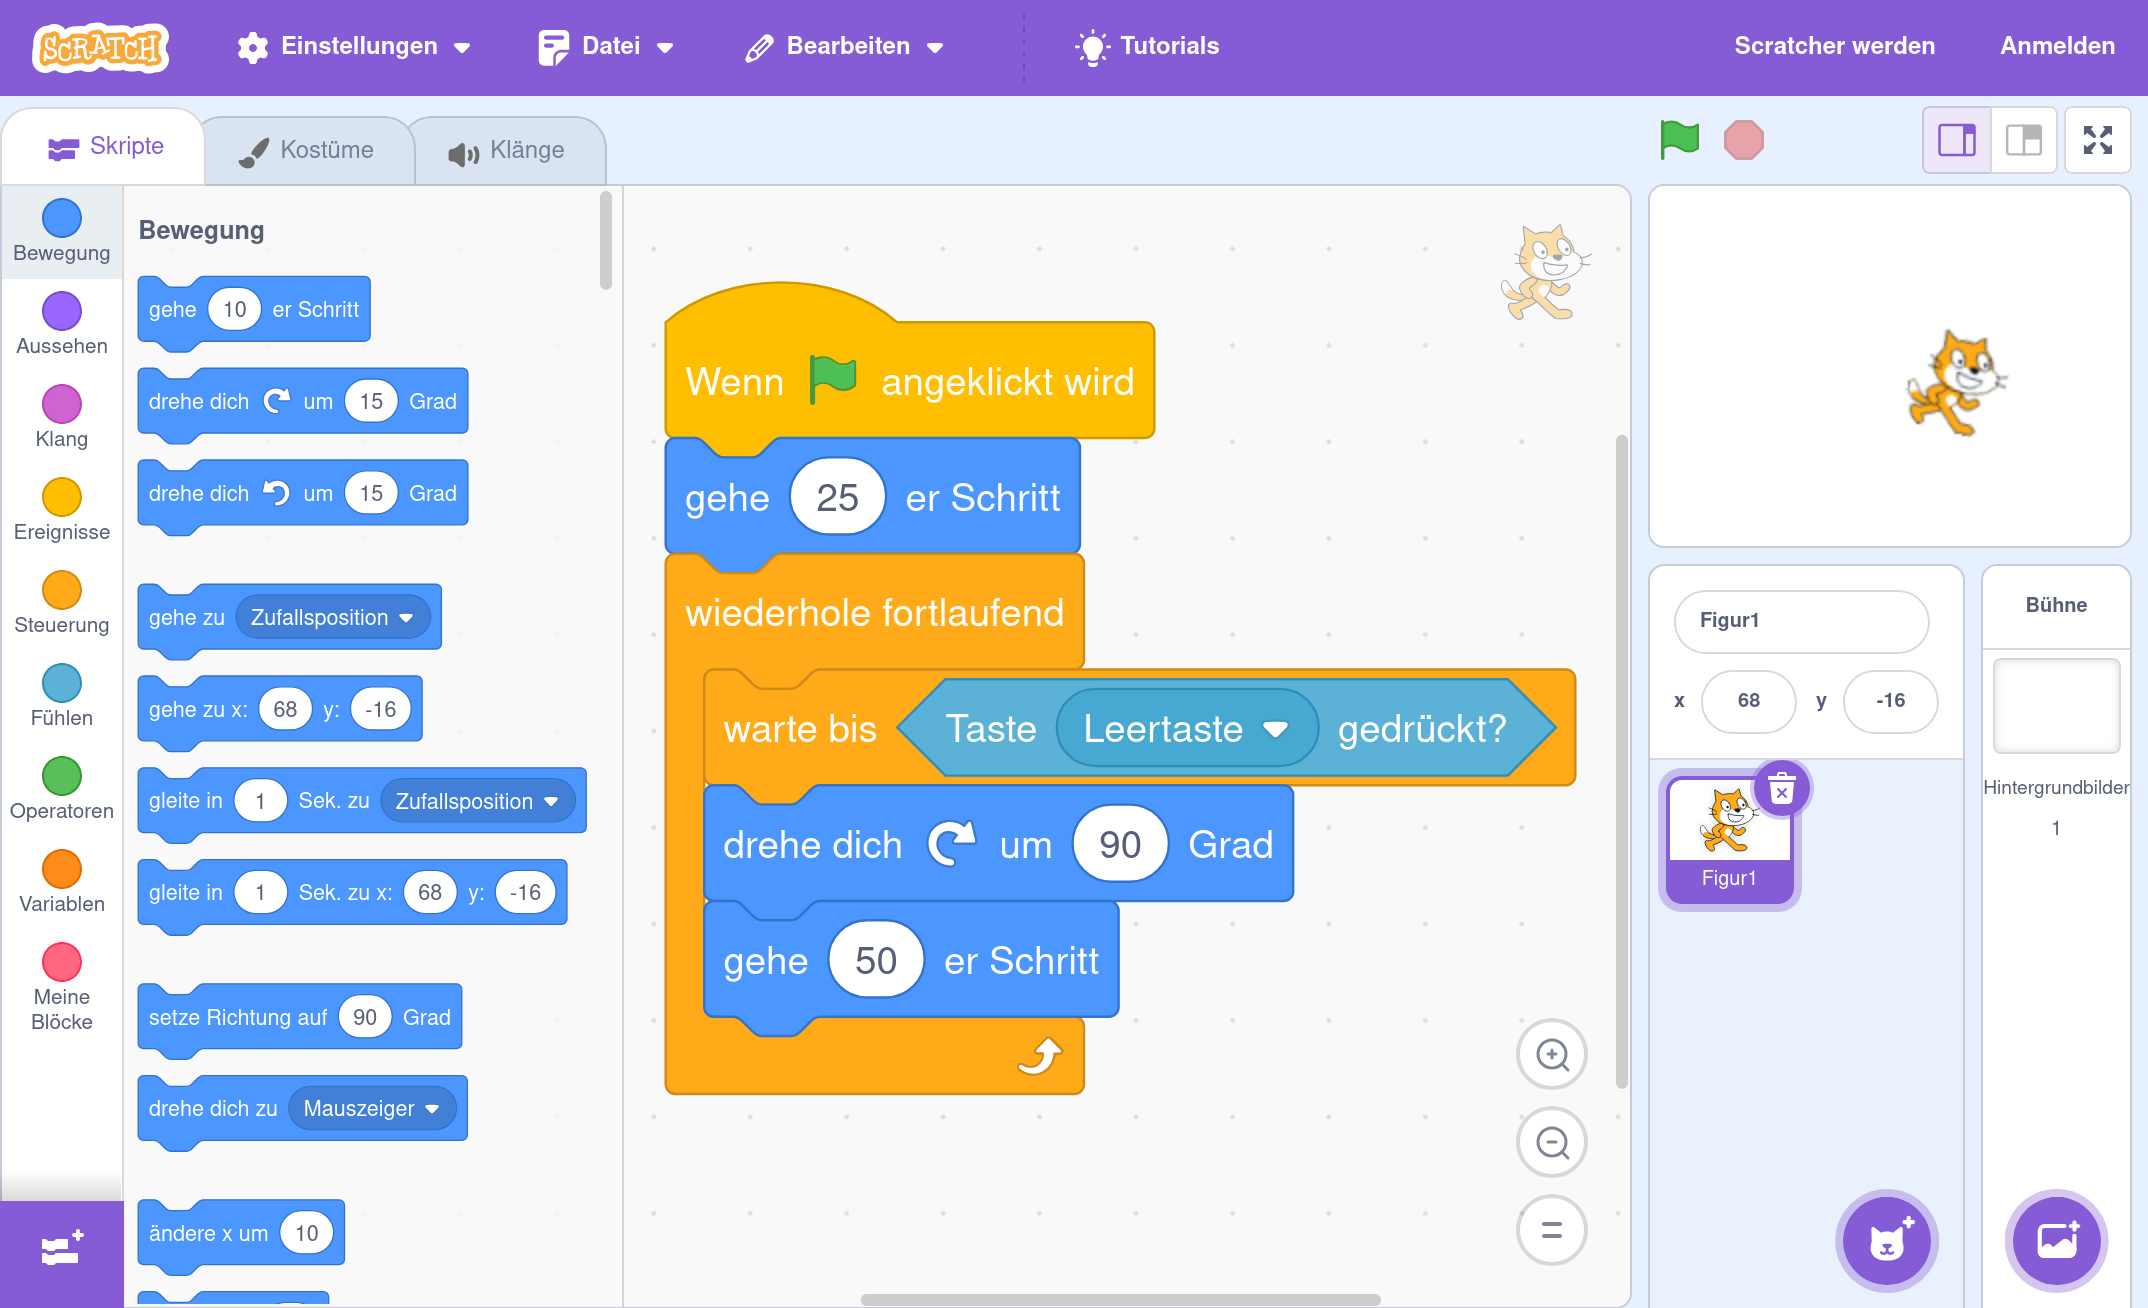
\includegraphics[width=0.95\textwidth]{assets/scratch.png}
  \end{center}
  \caption{Beispielprogramm in \Scratch{}. \parencitealias{scratchfoundationScratch}}
  \label{fig:scratch}
\end{figure}

Abbildung \ref{fig:scratch} zeigt den \Scratch{}-Editor und ein Beispielprogramm. Die Ansicht kann in 3 Spalten unterteilt werden. Links können die Blöcke ausgewählt werden, die in der Mitte zusammengesetzt werden sollen. Der rechte Abschnitt ist unterteilt, in einen Ausgabebereich, und ein Verwaltungsbereich für Figuren und Bühnen. Die Blöcke im Auswahlmenü sind thematisch sortiert. Die Farbgebung spiegelt dies wieder (Vgl. Abbildung \ref{fig:scratch-types}). Um Blöcke im Skriptbereich zu verwenden, müssen sie mittels \textit{Drag and Drop} nach rechts gezogen werden. Skripte sind an Figuren gebunden. Im Beispielprogramm wird die Tiger-Figur nach Start des Programms bewegt und rotiert, sobald die Leertaste gedrückt wird.
\parencite{maloneyScratchProgramming2010}

\begin{figure}
  \begin{center}
    
\includegraphics[width=0.95\textwidth]{assets/scratch-blocks.png}
  \end{center}
  \caption{Blockformen in \Scratch{} (v. l. n. r.): Befehl, Funktion, Auslöser, Kontrollstruktur. \parencitealias{scratchfoundationScratch}}
  \label{fig:scratch-blocks}
\end{figure}

\Scratch{} definiert grundsätzlich vier Blockformen \parencite{maloneyScratchProgramming2010}. In Abbildung \ref{fig:scratch-blocks} werden sie verglichen. \textbf{Befehle} führen Programmlogik aus, die beispielsweise Figuren bewegen oder Variablen anpassen. Sie besitzen typischerweise eine Kerbe am oberen Rand und Verbindungsstelle am unteren Rand. \textbf{Funktionen} geben Werte zurück, die errechnet werden können oder in Variablen gespeichert wurden. Es ist nicht möglich, Funktionen an Blöcke mit Kerben anzufügen, sie können aber in korrespondierende Felder innerhalb von Blöcken eingesetzt werden. \textbf{Auslöser} besitzen keine Kerbe am oberen Rand, und stellen den Anfang der Ausführung des angehängten Konstrukts dar. \textbf{Kontrollstruktur-Blöcke} haben die gleiche Form wie Befehle und können wie sie angewendet werden. Sie beeinflussen den Ablauf des Programms und bilden Programmierkonzepte wie Schleifen und Bedingungen ab. Abbildung \ref{fig:scratch} zeigt eine "wiederhole fortlaufend"-Schleife. Es ist zu sehen, dass diese Art von Block auch weitere Blöcke annehmen kann, die im Schleifenkörper ausgeführt werden.
\parencite{maloneyScratchProgramming2010}

\begin{figure}[!ht]
  \minipage[t]{.49\textwidth}
  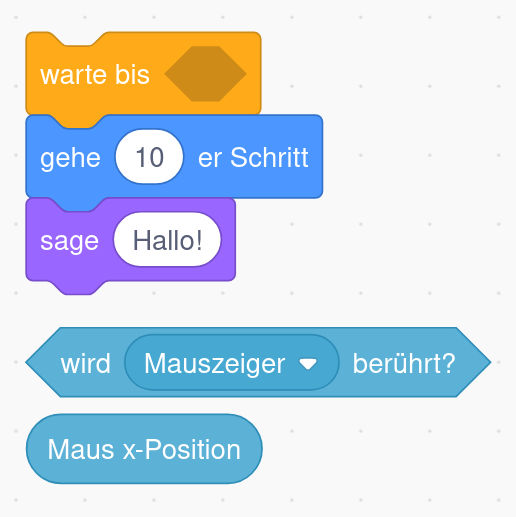
\includegraphics[width=\linewidth]{assets/scratch-types.png}
  \caption{Drei der Blockkategorien in \Scratch{}: Steuerung (Orange), Bewegung (Blau), Aussehen (Lila). Datentypen in \Scratch{}: Boolean (zugespitzte Blöcke), Zahlen und Text (abgerundete Blöcke). \parencitealias{scratchfoundationScratch}}
  \label{fig:scratch-types}
  \endminipage
  \hfill
  \minipage[t]{.49\textwidth}
  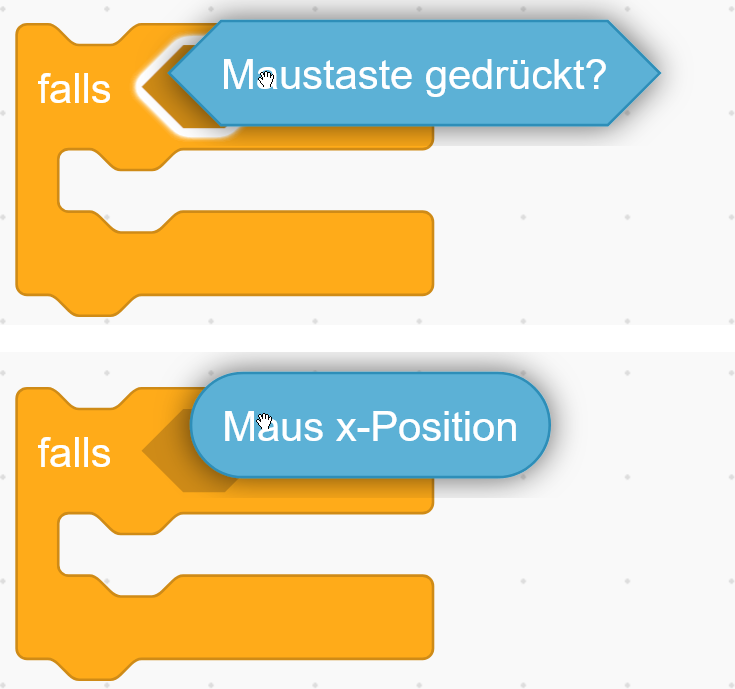
\includegraphics[width=\linewidth]{assets/scratch-drop.png}
  \caption{Blöcke können nur ineinander gesetzt werden, wenn der Datentyp übereinstimmt. Dies wird durch einen weißen Indikator vermittelt. \parencitealias{scratchfoundationScratch}\todo{ersetzen durch DIY Bild}}
  \label{fig:scratch-drop}
  \endminipage
\end{figure}

Die Programmiersprache \Scratch{} beschränkte sich zunächst auf drei Datentypen \parencite{maloneyScratchProgramming2010}. Dabei handelt es sich um Text, Zahl und Wahrheitswerte. Texte und Zahlen werden mit abgerundeten Ecken dargestellt, während Wahrheitswerte spitze Ecken besitzen. In Abbildung \ref{fig:scratch-types} werden zwei Funktionen mit unterschiedlichen Datentypen gezeigt, sowie Blöcke die diese als Eingabewerte entgegennehmen können. In den blauen und lila-farbigen Blöcken können auch manuell Werte eingegeben werden, der blaue Block nimmt jedoch nur Zahlen an. Die Datentypen in \Scratch{} wurden mit Nachfolgeversionen erweitert, Version 1.3 führte beispielsweise Listen ein \parencite{harveyBringingNo2010}.

\Scratch{} signalisiert über die Form der Blöcke, ob sie zusammengesetzt werden können. Zusätzlich wird beim \textit{Drag and Drop} über einen weißen Indikator gezeigt, ob Blöcke an der aktuellen Stelle eingesetzt werden können. In Abbildung \ref{fig:scratch-drop} ist zu sehen, wie so signalisiert wird, dass eine Wenn-Abfrage nur Wahrheitswerte annehmen kann.

Eine grundlegende Überlegung die bei der Entwicklung von \Scratch{} getroffen wurde, war das Verzichten auf Fehlermeldungen \parencite{maloneyScratchProgramming2010}. Nutzer:innen sollten anhand der Form der Blöcke erkennen, ob es möglich ist, Elemente miteinander zu kombinieren und durch probieren herausfinden, was funktioniert \parencite{maloneyScratchProgramming2010}.

\Scratch{} wird auch im Bildungsbereich genutzt, sowohl in Schulen \parencite{ortiz-colonTeachingScratch2016}, als auch an Universitäten \parencite{dekerekiScratchApplications2008}. Der Erfolg dieser Anwendung variiert, führt jedoch oft zu Motivationssteigerungen \parencite{dekerekiScratchApplications2008, martinez-valdesRelativelyUnsatisfactory2017}. Dies ist besonders bei jüngeren Zielgruppen der Fall \parencite{ortiz-colonTeachingScratch2016}.

\subsubsection{Snap!}
\Snap{} stellt eine Neuimplementierung von \Scratch{} mit neuen Funktionen dar. \textcite{harveyBringingNo2010} stellte in zeitigen Versionen von \Scratch{} Einschränkungen fest, die es für die Benutzung zur Lehre in der höheren Bildung ungeeignet macht. Einerseits gab es keine Funktionen und konnte somit keine Rekursion abbilden, andererseits wurden komplexe Datenstrukturen nicht unterstützt \parencite{harveyBringingNo2010}.

\begin{figure}[!ht]
  \minipage[t]{.57\textwidth}
  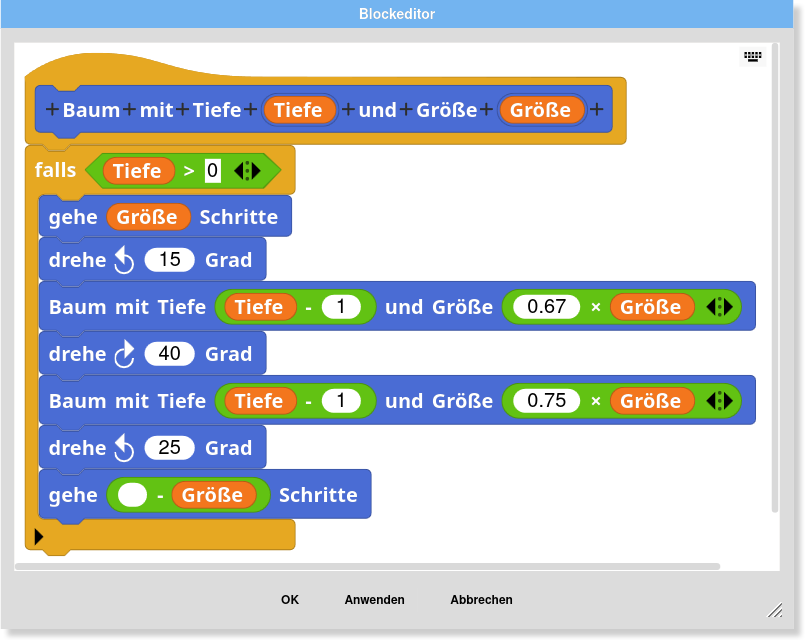
\includegraphics[width=\linewidth]{assets/snap-edit.png}
  \caption{Definition einer rekursiven Funktion in \Snap{}, am Beispiel von \textcite{harveyBringingNo2010}.}
  \label{fig:snap-edit}
  \endminipage
  \hfill
  \begin{minipage}[t]{.41\textwidth}
  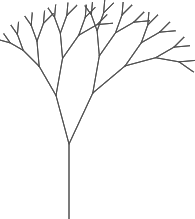
\includegraphics[width=\linewidth]{assets/snap-tree.png}
  \caption{Ergebnis der Funktion, wenn der Pfad aufgezeichnet wird.}
  \label{fig:snap-tree}
  \end{minipage}
\end{figure}

Um Rekursion in \Scratch{} umzusetzten, wurde eine Erweiterung namens \ac{BYOB} entwickelt, die es Nutzer:innen erlaubt, eigene Blöcke zu definieren \parencite{harveyBringingNo2010}. Später wurde diese Erweiterung zu einer eigenständigen Anwendung, \Snap{}, welche diese und weitere Funktionalitäten enthält. Abbildungen \ref{fig:snap-edit} und \ref{fig:snap-tree} zeigen die Definition und das Ergebnis einer rekursiven Funktion, die als Block definiert wurde, und sich somit selbst aufrufen kann.

\Snap{} verallgemeinert die Datentypen von \Scratch{} und ermöglicht somit tiefgreifenderen Zugriff auf Variablen. So ist es zum Beispiel möglich, über den Listen-Block Listen zu erstellen, die nicht zuvor als Variable definiert werden müssen. Das ermöglicht Listen in Listen und komplexere Datentypen \parencite{harveySnapReference2020}.

Außerdem unterstützt \Snap{} Ansätze der funktionalen Programmierung, indem Funktionen als Daten übergeben werden können. Ein Beispiel dafür stellt der "Wende ... an auf ...", welches eine Funktion im ersten Parameter entgegennimmt und auf alle Elemente der Liste im zweiten Parameter anwendet \parencite{harveySnapReference2020}. Diese Möglichkeit, gekoppelt mit Blöcken zum Klonen von Figuren und Funktionen, ermöglicht wiederum objektorientierte Programmierung innerhalb von \Snap{} \parencite{harveySnapReference2020}. Figuren werden in \Snap{} auch als Objekte bezeichnet.

\begin{figure}
  \centering
    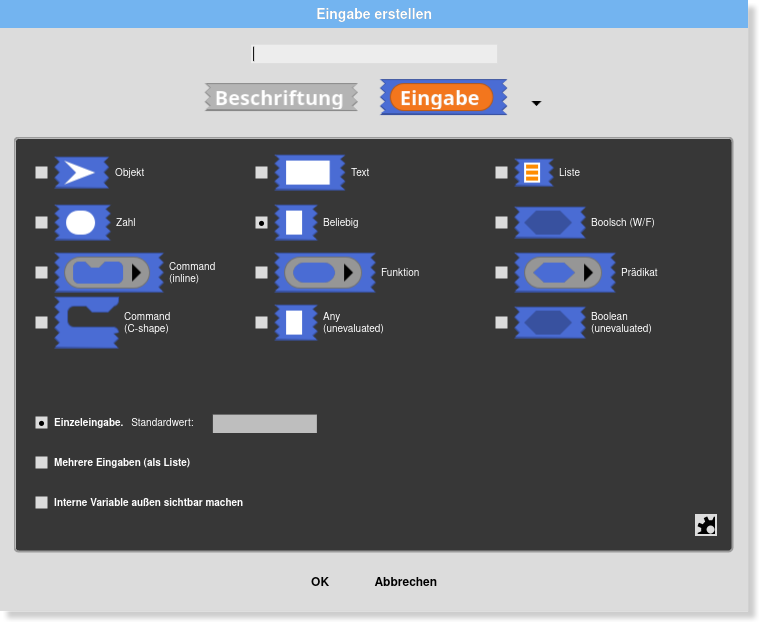
\includegraphics[width=0.57\textwidth]{assets/snap-input-types.png}
  \caption{Ausführlicher Dialog zur Definition eines Parameters.}
  \label{fig:snap-input-types}
\end{figure}

Wie in Abbildung \ref{fig:snap-input-types} zu sehen, unterstützt der Editor für Eingabeparameter von Blöcken unterschiedliche Parametertypen. Somit können während der Erstellung eines Blocks die Einstellungen so gewählt werden, dass die Bedienung des Blocks erleichtert wird. \Snap{} kennt die Eingabetypen des Blocks und kann somit sicherstellen, dass nur passende Blöcke in die Eingabefelder eingesetzt werden \parencite{harveySnapReference2020}. \Snap{} erweitert den in Abbildung \ref{fig:scratch-drop} gezeigten Ansatz, indem beim \textit{Drag and Drop} ein roter Indikator angezeigt wird, wenn der Typ nicht übereinstimmt \parencite{harveySnapReference2020}.

Während das Aussehen der \Snap{}-Programmierumgebung \Scratch stark ähnelt, wurde \Snap{} mit einigen Funktionalitäten angereichert, die dazu führen, dass komplexe Konzepte der Programmierung in einem blockbasierten Editor erlernt werden können \parencite{ballSnapLook2019}. Eingesetzt wird es beispielsweise im Kurs \textit{"The Beauty and Joy of Computing"} der \citeauthor{universityofcaliforniaberkeleySnapBuild}, welcher sich an Studiengänge außerhalb der Informatik richtet \parencite{universityofcaliforniaberkeleySnapBuild}.

\subsubsection{DataSnap}
- 4 eigenschaften des papers erklären (p. 19) (und zwei abschnitte oben drüber)
- komplexere Blöcke vordefinieren (p. 26)

- bilder mit blöcken und so (ist das definieren ein snap feature??? - BYOB!)

\begin{figure}[!ht]
  \centering
    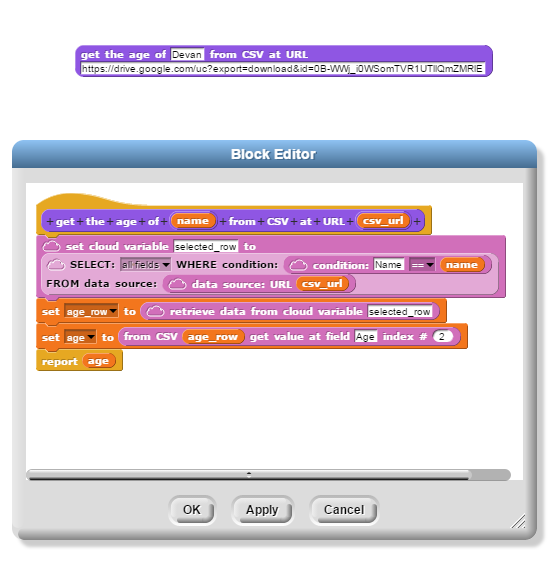
\includegraphics[width=0.95\textwidth]{assets/datasnap-block-definition.png}
  \caption{Anlegen einer Abfrage zur späteren Wiederverwendung. \parencite{hellmannDataSnapEnabling2015}}
  \label{fig:datasnap-block-definition}
\end{figure}

\begin{figure}[!ht]
  \centering
    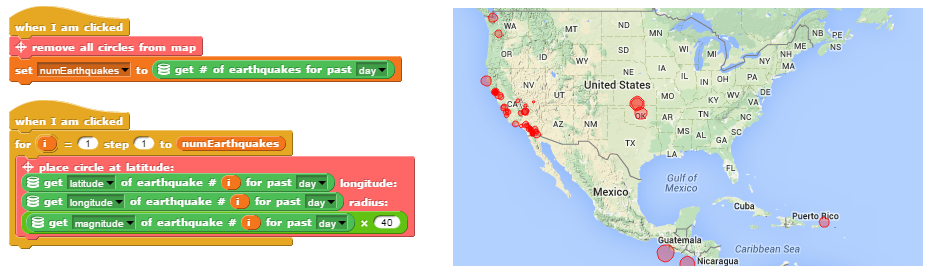
\includegraphics[width=0.95\textwidth]{assets/datasnap-visualization.png}
  \caption{Visualisierung eines Datensatzes über Erdbeben in DataSnap. \parencite{hellmannDataSnapEnabling2015}}
  \label{fig:datasnap-visualization}
\end{figure}

- inwiefern unterscheidet sich datasnap von s4d projekt?


\parencite{hellmannDataSnapEnabling2015} (Chapter 3: DataSnap for Domain Experts)
- based on Snap! 
  - inspired by scratch 


\chapter{Entwicklung und Usability-Studie}
\section{Prototyp}

\subsection{Zielformulierung}\todo[noline]{ganz schöne oft "Ausgangsdaten"}

Ziel ist es, eine Anwendung zu schaffen, welche den Anforderungen der Datenverarbeitung innerhalb von Simplex4Data gerecht wird. Dabei gibt es zwei Anwendungsbereiche, welche sich aber in ihren Grundeigenschaften ähneln: das Erstellen von Konvertierungen beim Importieren in das Realitätsmodell (Vgl. \ref{sec:simplex-importer}) und das Erstellen von SimplexSzenarios (Vgl. \ref{sec:simplex-scenarios}).

Das Erstellen von Konvertierungen ist der zweite Schritt beim Importieren in das Realitätsmodell. Im ersten Schritt werden die Ausgangsdaten aus Dateien oder APIs ausgelesen, und in Datenbanktabellen geschrieben. Dabei entstehen sogenannte Quelltabellen, in denen die Informationen in flachen Strukturen enthalten sind. Die Konvertierungen nutzen die Quelltabellen dann, um die Daten in das Realitätsmodell zu übertragen.

Sobald die Daten sich im Realitätsmodell befinden, ist es möglich, SimplexSzenarios zu definieren. Diese selektieren und kombinieren Attribute aus Objektklassen, um fachspezifische Auswertungen zu generieren.

Beide Prozesse erfordern manuelle Angaben, die bestimmen wie aus den Ausgangsdaten (Quelltabellen oder Objektklassen) Zielstrukturen (Objekte oder SimplexSzenarios) erstellt werden sollen. In beiden Fällen ist das Format der Ausgangsdaten wohl-definiert, da Attribut-Schlüssel und Datentypen gegeben sind. Im Falle der Konvertierungen ist auch das Zielformat festgesetzt, da die Attribute der Objektklasse bereits definiert wurden. Bei SimplexSzenarios ist dies nicht der Fall, die darin enthaltenen Attribute können frei spezifiziert werden. Sowohl in Konvertierungen als auch SimplexSzenarios ist es möglich, Funktionen auf Attribute, beziehungsweise Datenbankspalten anzuwenden. Dabei handelt es sich um Standard-\ac{SQL}-Funktionen oder solche, die durch Erweiterungen\footnote{wie beispielweise PostGIS, eine PostgreSQL-Erweiterung für Geodaten \parencite{postgispscPostGIS}} zur Verfügung gestellt werden. Außerdem können im Zuge beider Arbeitsschritte Filterbedingungen definiert werden, um nur bestimmte Zeilen der Quelltabelle in Objekte umzuwandeln oder um nur bestimmte Objekte in SimplexSzenarios auszuwerten.

Aufgrund der genannten Gemeinsamkeiten soll ein Editor entwickelt werden, welcher sowohl für die Erstellung von Konvertierungen als auch für die Definition von SimplexSzenarios verwendet werden kann. Im zweiten Anwendungsfall unterscheidet sich die Funktionalität dahingehend, dass die Ausgabefelder frei bestimmt und benannt werden können.

\begin{figure}[ht]
  \centering
  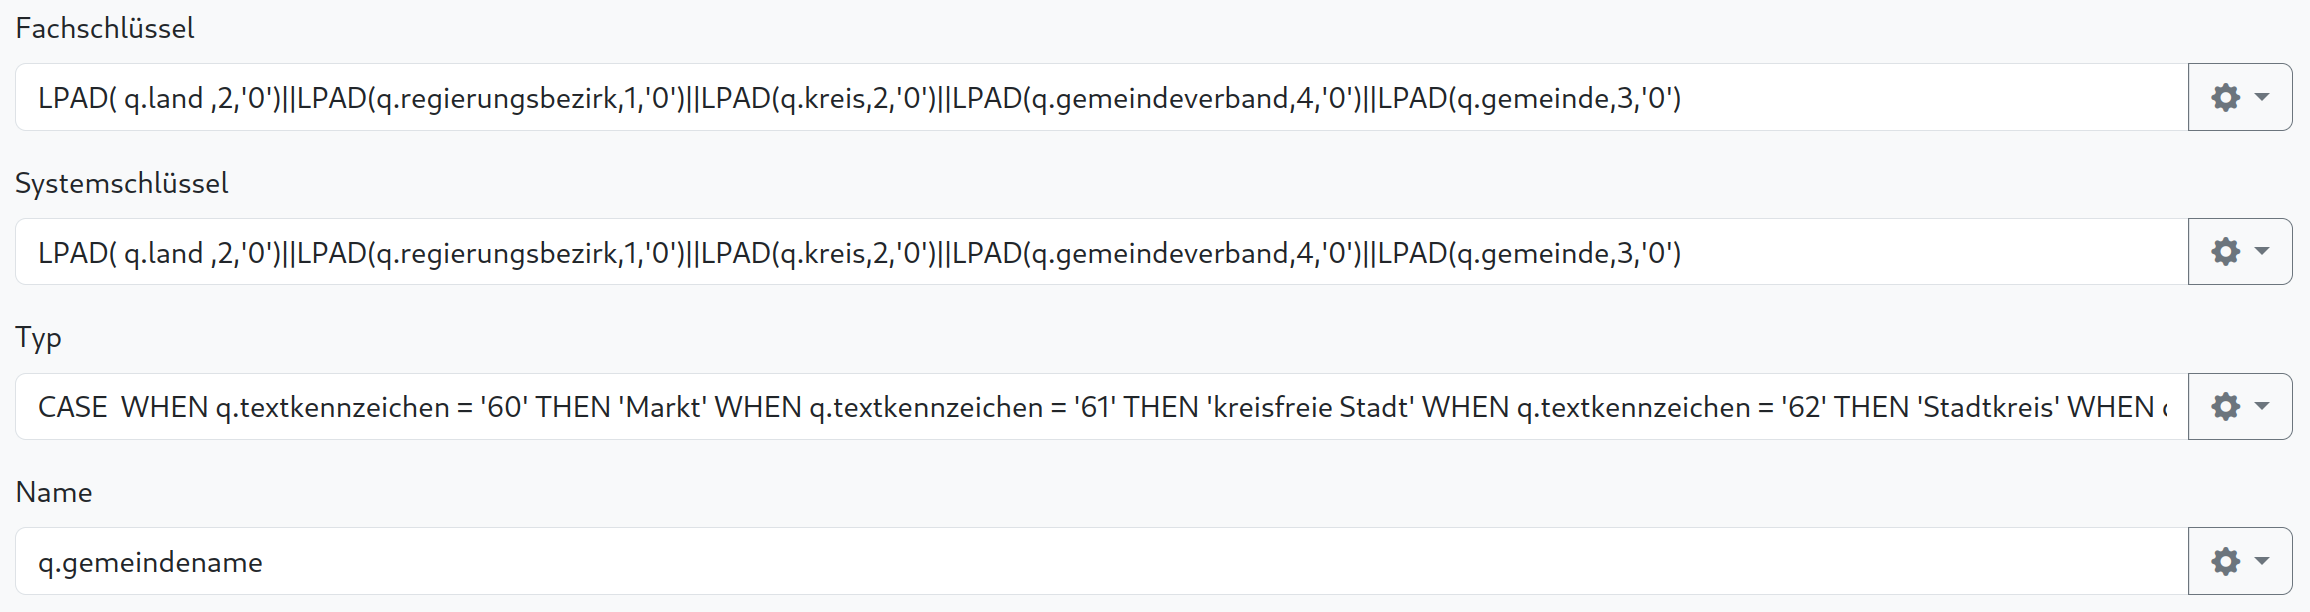
\includegraphics[width=.95\textwidth]{assets/conversion-gemeinde.png}
  \caption{Auszug aus der Konvertierungsdefinition für die Objektklasse "Gemeinde" im aktuellen Editor für Konvertierungen.}
  \label{fig:conversion-gemeinde}
\end{figure}

Der aktuelle Editor für Konvertierungen besteht aus Textfeldern, in denen Auszüge von \ac{SQL}-Befehlen eingegeben werden können. Ein Beispiel dafür ist in Abbildung \ref{fig:conversion-gemeinde} gegeben. Für jedes Attribut wird dies dann in einem \texttt{SELECT}-Befehl eingesetzt. Diese Herangehensweise ist äußerst flexibel, weißt jedoch in der Benutzung einige Usability-Probleme auf: Erstens sind die Ausgangsdaten nicht innerhalb des Editors dokumentiert.\todo[noline]{mehr auf bild eingehen?} Die Benutzer:innen müssen somit immer nachschlagen, welche Werte sie eintragen können. Das manuelle Eintippen birgt außerdem die Gefahr, sowohl Tippfehler als auch Fehler im \ac{SQL}-Syntax zu verursachen. Auch die inhaltliche Sinnhaftigkeit der Befehle wird nicht sichergestellt, und Nutzer:innen, die nicht vertraut mit SQL sind, benötigen aufwendige Einführungen und können komplexe Aufgaben schlechter bewältigen. \todo[noline]{oh oh alles nicht belegt}

Der entwickelte Editor sollte in Sachen Nutzbarkeit eine Verbesserung gegenüber der aktuellen Lösung darstellen. Es sollte weniger Nachschlagearbeit nötig sein, weniger Tippfehler auftreten und auch für Personen, die keinen technischen Hintergrund oder \ac{SQL}-Vorkenntnisse besitzen, nutzbar sein.

Zusammenfassend können folgende Ziele formuliert werden:
\begin{itemize}
  \item Entwicklung eines Editors für Konvertierungen und SimplexSzenarios.
  \item Der Editor soll häufiges Nachschlagen verhindern.
  \item Der Editor soll Tippfehlern vorbeugen.
  \item Der Editor soll auch ohne \ac{SQL}-Kenntnisse bedienbar sein.
\end{itemize}

\subsection{Der Block-Editor}

Es wurde sich für die Entwicklung einer Low-Code-Oberfläche entschieden, in der einzelne Elemente als Blöcke dargestellt werden. Wie diese bei der Bearbeitung von Konvertierungen aussieht, ist in Abbildung \ref{fig:buffet-simple} zu sehen. Der Informationsfluss wurde von links nach rechts konzipiert, sodass links die Ausgangsdaten zu finden sind, die rechts eingetragen werden können.

Im linken Bereich befinden sich sowohl die abfragbaren Tabellenspalten (als "Abfragbare Felder" bezeichnet), als auch Funktionen. Über diesen beiden Abschnitten sind Schaltflächen zum Filtern untergebracht, sodass die abfragbaren Felder oder Funktionen wahlweise ausgeblendet werden können. Die Elemente werden als große Schaltflächen dargestellt und enthalten relevante Informationen: Der Datentyp wird als Text (grau, oben links) und als Symbol (rechts) angezeigt. Bei Funktionen handelt es sich hierbei um den Rückgabetyp. Abfragbare Felder weisen ihre Namen und Schlüssel auf (z.B. "Bevölkerung" und "bevoelkerung"), während Funktionen über einen Namen und eine Beschreibung verfügen (z.B. "=" und "Gleichheitsprüfung"). Durch diese Auflistung soll das Nachschlagen und Eintippen von Elementen durch ein einfaches Auswählen ersetzt werden.

\begin{figure}[ht]
  \centering
  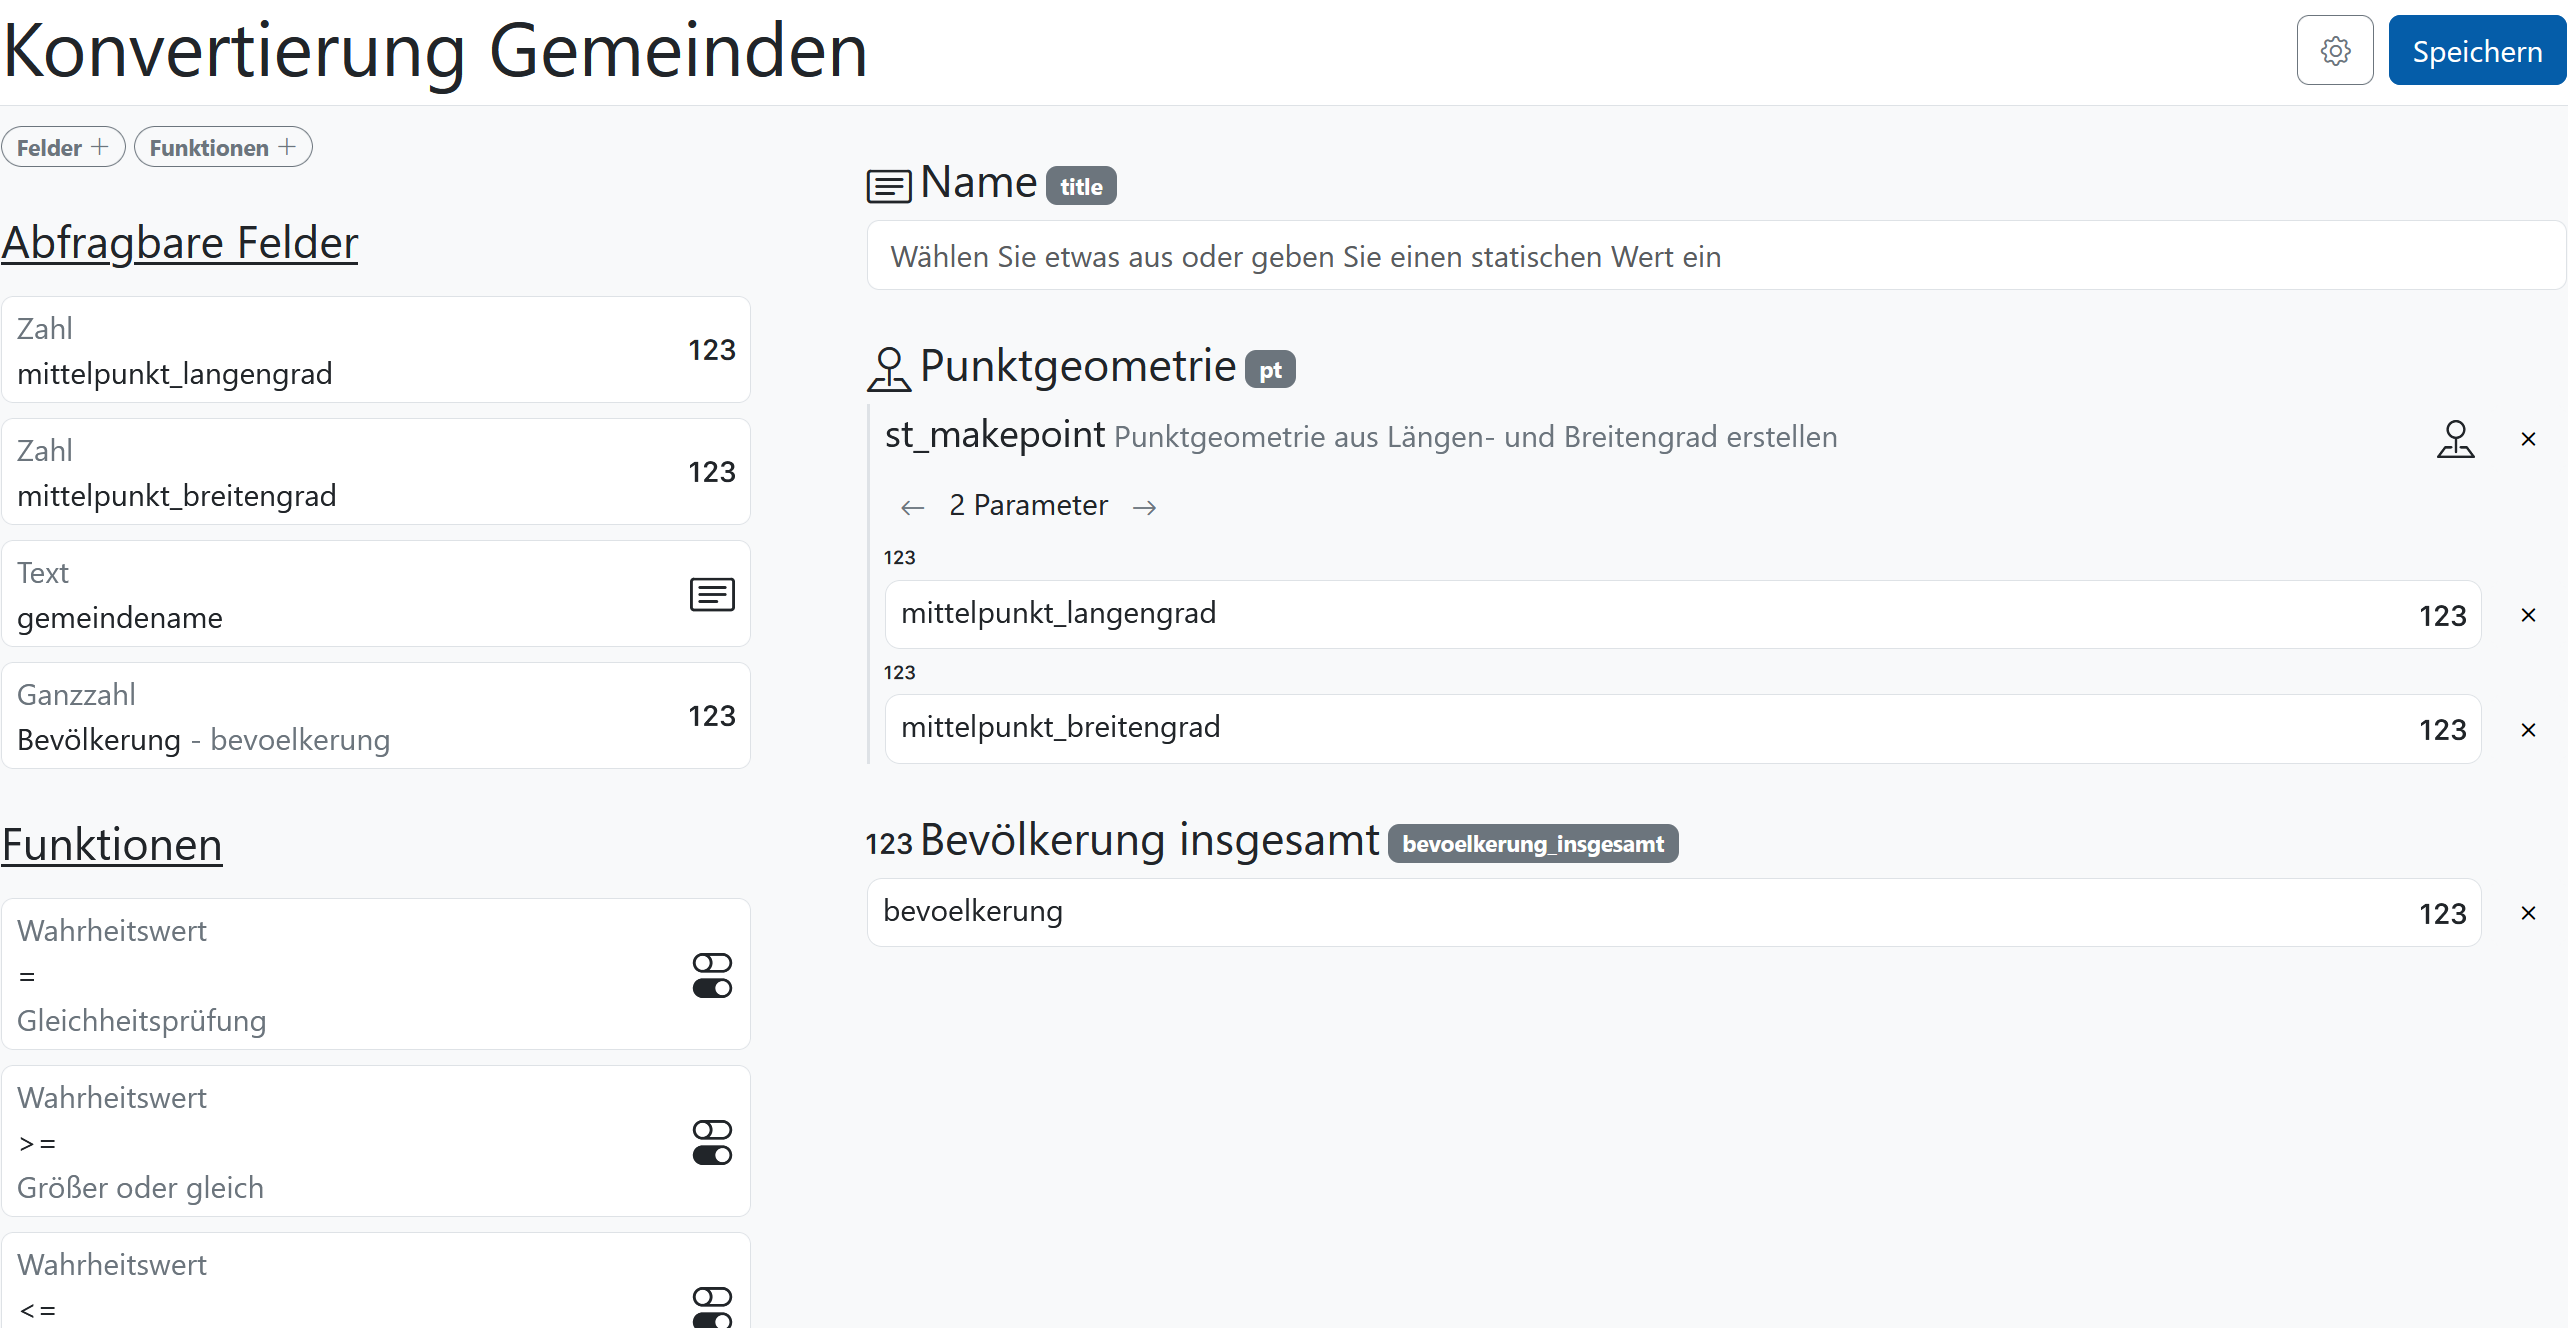
\includegraphics[width=.95\textwidth]{assets/buffet-simple.png}
  \caption[Verwendung des Block-Editors zur Erstellung einer Konvertierung]{Verwendung des Block-Editors zur Erstellung einer Konvertierung der Objektklasse "Gemeinde". Bereits ausgefüllt sind die Attribute "Punktgeometrie" und "Bevölkerung insgesamt", während das Standardfeld "Name" noch mit den Auswahlmöglichkeiten im linken Menü befüllt werden muss.}
  \label{fig:buffet-simple}
\end{figure}

Im rechten Bereich der Oberfläche wird die Zielstruktur dargestellt. Bei Konvertierungen wird diese durch die Klassendefinition vorgeschrieben. Die Eingabemaske für die einzelnen Attribute besteht aus einem Symbol für den Datentyp, dem Attribut-Name und -Schlüssel, sowie einem dem Datentyp angepassten Eingabefeld. Sobald ein Eingabefeld mit einer Auswahl befüllt wurde, besteht die Möglichkeit, diese wieder durch die Schaltfläche am rechten Rand zu entfernen. Falls das Feld durch eine Funktion gebildet werden soll, muss zuerst die Funktion ausgewählt werden, wodurch wiederum zu Parametern korrespondierende Eingabefelder entstehen. Diese können dann analog mit Attributen oder Funktionen befüllt werden. Somit ist es möglich, beliebig komplexe Schachtelungen zu erstellen\footnote{Eine Obergrenze für den Grad der Schachtelung könnte maximal durch begrenzten Bildschirmplatz erreicht werden. Da pro Schachtelung nur wenig horizontaler Platz verloren geht, wird angenommen, dass diese Grenze höher liegt, als in der Praxis benötigt.}. Die Zusammengehörigkeit von Parametern und Funktionen wird durch einen vertikalen Strich an der linken Seite dargestellt. Abbildung \ref{fig:buffet-scenario} zeigt, wie dies mit einer komplexeren Abfrage aussieht.

Die dargestellten Datentypen erfüllen nicht nur eine informative Funktion, sondern sind auch inhaltlich relevant. Felder können nur mit Elementen befüllt werden deren Datentyp übereinstimmt. Somit soll ein Minimum an Korrektheit der Abfragen sichergestellt werden. Außerdem wird diese Einschränkung dazu genutzt, die Zuordnungsmöglichkeiten zu reduzieren. Wird auf das zu einem Attribut gehörige Eingabefeld geklickt, wird der Auswahlbereich links auf Elemente des Datentyps des Attributs gefiltert. Dies ist anhand des Attributs "Name" in Abbildung \ref{fig:buffet-selected} zu sehen. Umgedreht ist es auch der Fall: Wird links ein Attribut oder eine Funktion angeklickt, werden rechts die Felder ausgegraut, in die die Auswahl nicht eingefügt werden kann. Somit ist es im entwickelten Editor sowohl möglich, zuerst die Ausgangsdaten auszuwählen oder zuerst das Zielfeld.

\begin{figure}[ht]
  \begin{center}
    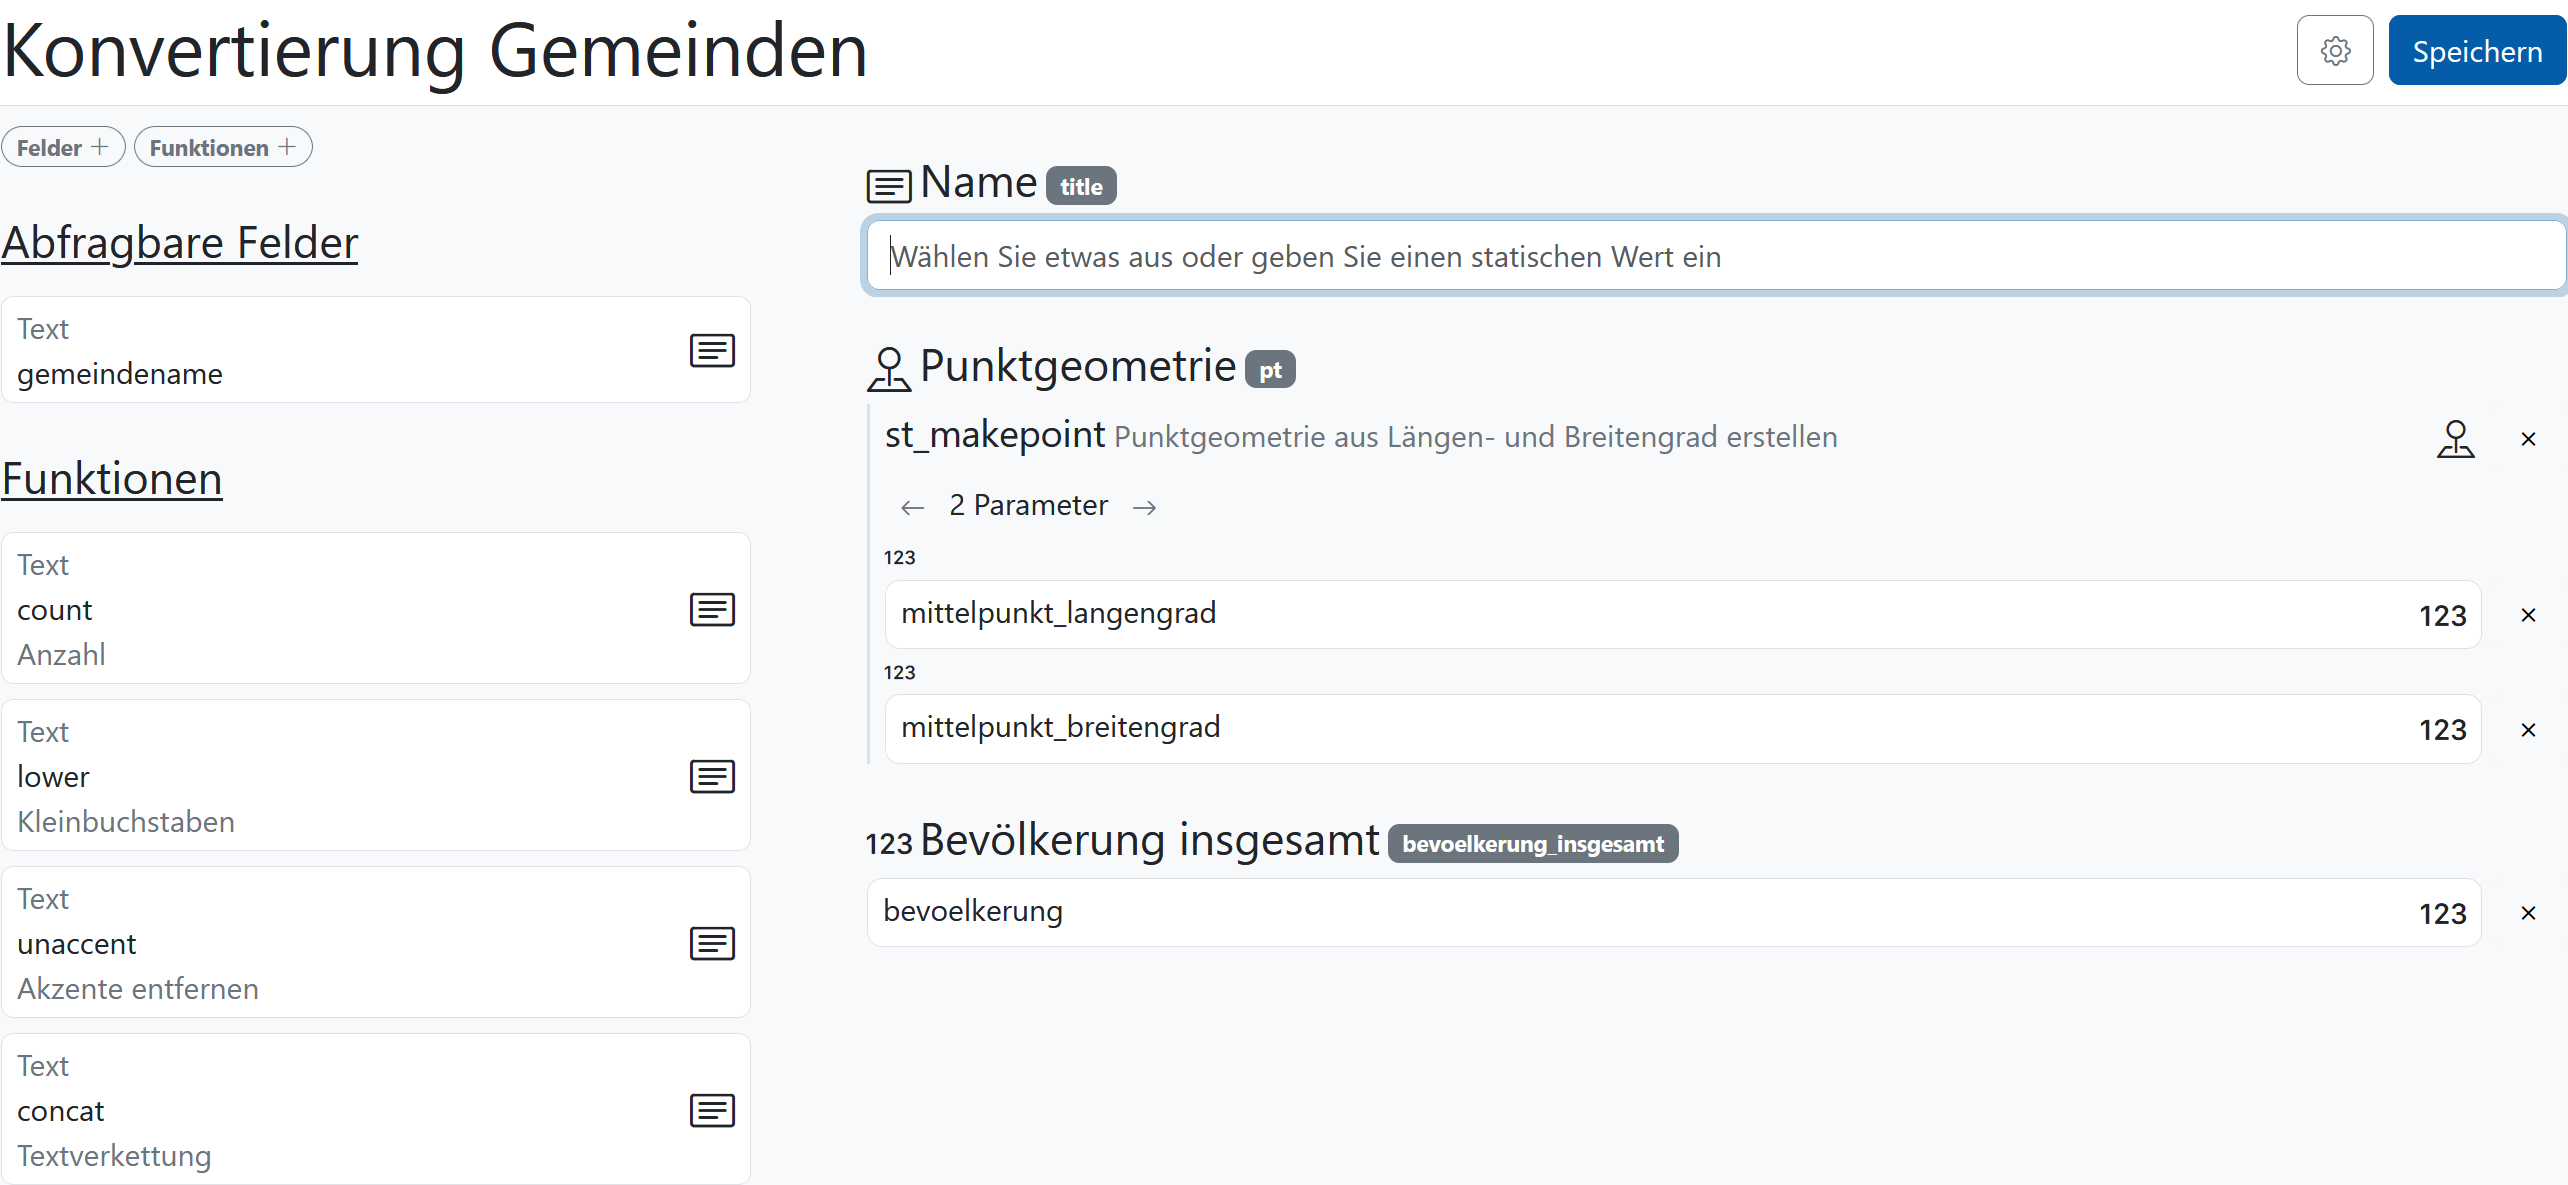
\includegraphics[width=.95\textwidth]{assets/buffet-selected.png}
  \end{center}
  \caption[Erstellung einer Konvertierung im Block-Editor mit aktivem Typfilter]{Erstellung einer Konvertierung der Objektklasse "Gemeinde". Das Standardfeld "Name" ist ausgewählt, wodurch sich die Auswahlmöglichkeiten im linken Menü auf relevante Einträge filtern.}
  \label{fig:buffet-selected}
\end{figure}

Der Block-Editor kann auch verwendet werden, um SimplexSzenarios zu erstellen. Dabei werden mehrere Bedienelemente hinzugefügt. In Abbildung \ref{fig:buffet-scenario} wird die Definition eines SimplexSzenarios gezeigt. Dabei wurden zuvor bereits die relevanten Klassen ("Blockseite" und "Fassadenpunkt") ausgewählt. Ein wichtiger Unterschied zu Konvertierungen besteht darin, dass die abfragbaren Felder aus den Attributen mehrerer Klassen bestehen. Diese unterscheiden sich einerseits im Präfix ihrer Schlüssel, andererseits wurde zur schnellen Identifizierung auch eine farbliche Anpassung vorgenommen. Sowohl das Symbol für den Datentyp, als auch die Umrandung sorgen für eine farbliche Sortierung der Objektklassen. Diese Farben werden auch im Kopf des linken Bereichs widergespiegelt, dort kann nun analog zum Elementtyp (Felder oder Funktionen) auch nach Klassen gefiltert werden. Im Beispiel (Abbildung \ref{fig:buffet-scenario}) wird eine fachspezifische Abfrage generiert, die die maximalen Lärmwerte entlang von Blockseiten aggregiert.

\begin{figure}[ht]
  \begin{center}
    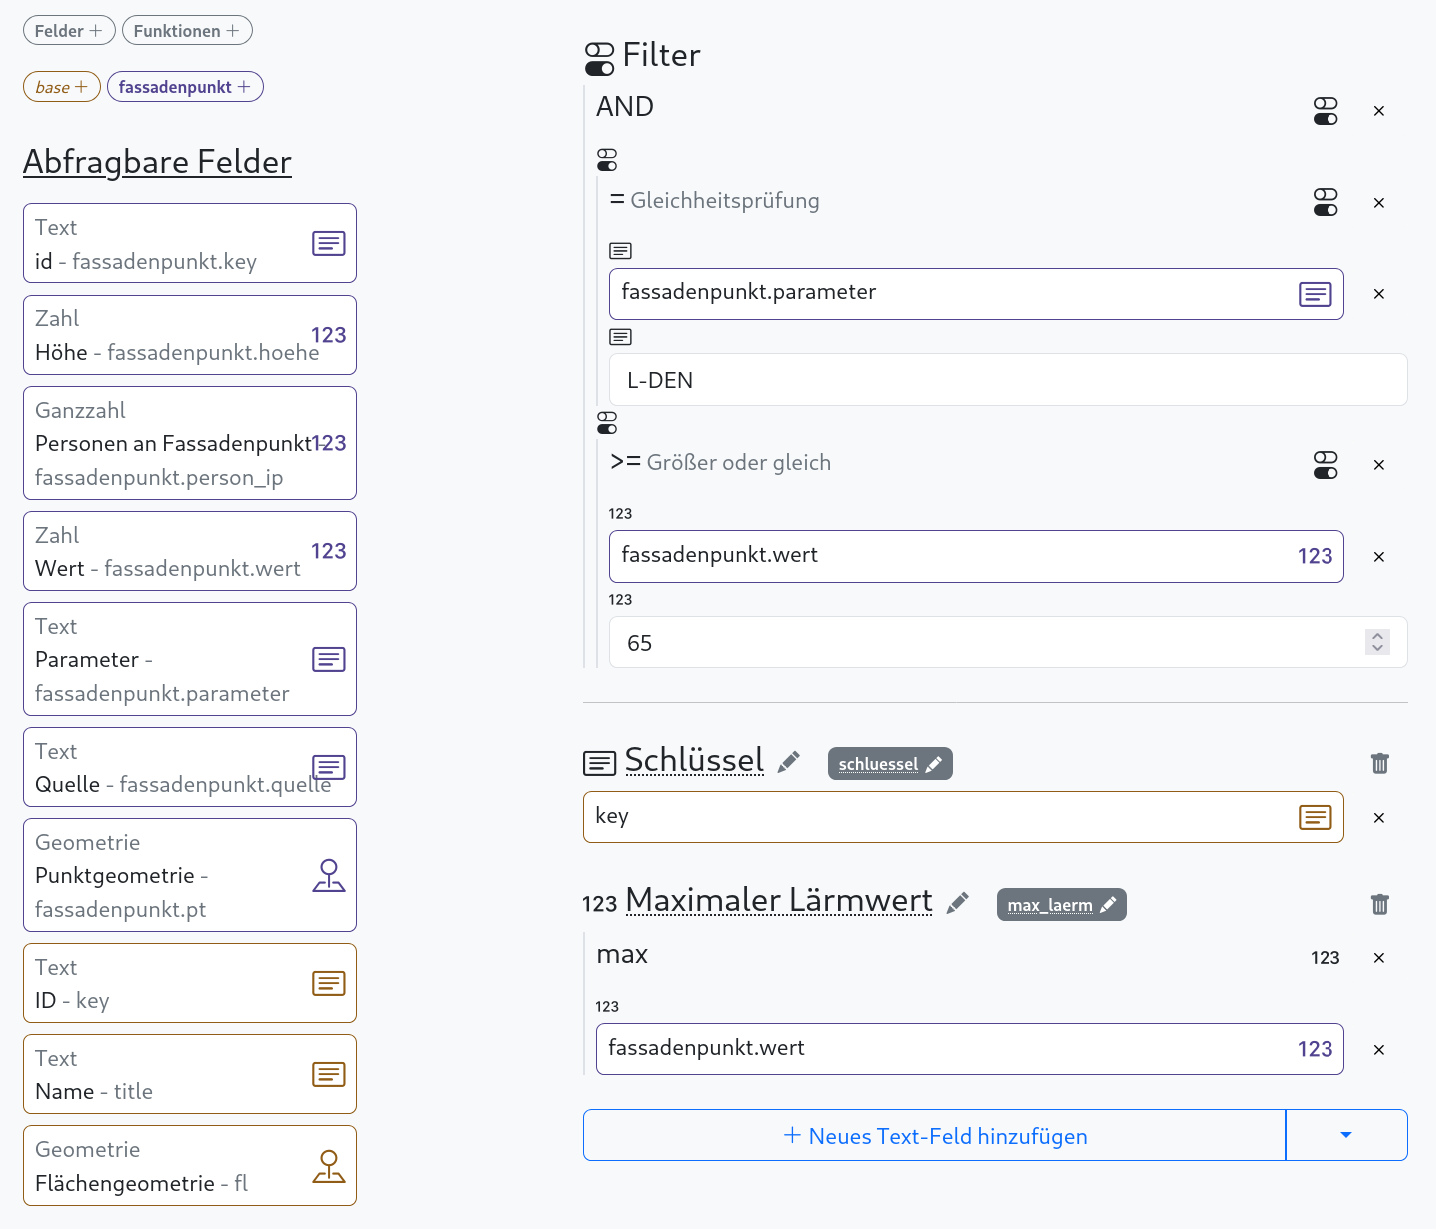
\includegraphics[width=.95\textwidth]{assets/lpz-scenario.png}
  \end{center}
  \caption[Verwendung des Block-Editors zur Erstellung eines SimplexSzenarios]{Verwendung des Block-Editors zur Erstellung eines SimplexSzenarios. In diesem Beispiel werden alle Blockseiten ausgewählt, deren maximaler Lärmwert an einem der zugeordneten Fassadenpunkte im Parameter \acf{LDEN} 65 Dezibel überschreitet.}
  \label{fig:buffet-scenario}
\end{figure}

Des Weiteren verfügt der Block-Editor im Szenario-Modus über einen Button, um neue Felder hinzuzufügen. Dabei muss bereits der gewünschte Datentyp gewählt werden. Während standardmäßig Felder vom Typ Text hinzugefügt werden, können die anderen Datentypen über ein Dropdown-Menü ausgewählt werden.

Sowohl der Titel als auch der Schlüssel von kreierten Feldern kann bearbeitet werden. Die Darstellung ist die gleiche wie bei Konvertierungen, mit dem Unterschied, dass die editierbaren Informationen gepunktet unterstrichen sind und ein Stift-Symbol daneben angezeigt wird.

\subsection{Technische Umsetzung}
\todo[noline]{welche infos sind hier zu kurz gekommen?}
Der Block-Editor gliedert sich in die restliche Anwendung, Simplex4Data, ein. Dabei wird die Serveranwendung unter Verwendung von Python und dem Django-Framework \parencite{djangosoftwarefoundationDjango} programmiert. Das Frontend ist eine Browser-Anwendung, die mit \ac{HTML}, JavaScript und \ac{CSS} (\ac{SASS}) umgesetzt wurde.

Das Backend generiert \ac{HTML}, welches an den Client gesendet wird. Da es sich bei dem vorliegenden Editor jedoch um eine sehr dynamische Anwendung handelt, wird nur ein Grundgerüst auf dem Server gebildet. Auf dem Client wird per \ac{API} abgefragt, welche abfragbaren Felder, Funktionen und auszufüllende Felder existieren. Aus dem so erhaltenen \ac{JSON} werden dann UI-Elemente mit Nunjucks \parencite{mozillaNunjucks} generiert. Des Weiteren wurde die JavaScript-Bibliothek jQuery \parencite{openjsfoundationJQuery} genutzt, um Zustände zu verwalten und auf Interaktionen zu reagieren.

Die für die Funktionsweise benötigten Daten stammen komplett aus dem \textit{API - Features} Dienst \parencite{ogcAPI} von Simplex4Data. Simplex4Data speichert die in den Quelltabellen enthaltenen Spalten und die Attribute der Objektklasse, inklusive Metadaten wie Titel, Schlüssel, Beschreibung und Datentyp. Diese werden über den \ac{API}-Endpunkt \texttt{/queryables} ausgegeben (Vgl. \ref{sec:queryables}). Somit ist es möglich, bei Konvertierungen den korrespondierenden Endpunkt der Quelltabelle anzufragen, sowie den der Objektklasse, um sowohl die Metadaten der Ausgangsdaten, als auch die der Zielstruktur abzufragen. Gleichweise kann beim Editieren von Szenarien der \texttt{/queryables}-Endpunkt der dazugehörigen Objektklassen genutzt werden, um die relevanten abfragbaren Felder zu bestimmen. Simplex4Data hat für diesen Zweck den \textit{API - Features} Dienst erweitert, um die Attribute mehrerer, miteinander verbundener Objektklassen auszugeben. Bei diesem Schritt werden auch die Präfixe, abhängig von der Objektklasse, gesetzt.

Auch die im Editor nutzbaren Funktionen werden aus der \ac{API} abgerufen, vom \texttt{/functions}-Endpunkt (Vgl. \ref{sec:functions}).
\todo[inline]{how do types differ between queryables and functions? information loss?}

Bildungsvorschriften, welche im Block-Editor erstellt werden, werden in \ac{CQL} verwaltet und im Anschluss an den \ac{API}-Dienst geschickt. Laut \citetitle{ogcFiltering} müssen konforme Dienste die Möglichkeit unterstützen, mit \ac{CQL} zu filtern. Simplex4Data bietet außerdem die Möglichkeit an, in \ac{API}-Abfragen Ausgabefelder zu definieren. Somit kann der komplette Funktionsumfang des Editors mit der \ac{API} abgebildet werden.

\subsection{Kritik}
\label{sec:criticism}

Im Zuge dieser Arbeit wurde der Block-Editor nicht komplett fertig programmiert. Er noch nicht in das restliche System Simplex4Data integriert, über den Editor erstellte Konvertierungen und Simplex-Szenarien können nicht abgespeichert oder zu Beginn der Bearbeitung eingelesen werden. Dies wird vor einer endgültigen Integration noch umgesetzt werden müssen, beeinflusst aber nicht das Testen des Konzepts in diesem Rahmen. Des Weiteren wurden einige offene Funktionalitäten identifiziert, die in geringerem Maße zur grundlegenden Herangehensweise der blockbasierten Datenverarbeitung beitragen und somit als weniger relevant erachtet wurden. Das Fehlen dieser Funktionalitäten könnte die Einfachheit der Nutzung jedoch herabsetzen.

Dazu gehört zum Beispiel das Umsortieren von bereits definierten Strukturen. Es ist nicht möglich, einen definierten Block zu verschieben, zu kopieren, oder ausgefüllte Parameter zu tauschen. Somit könnte es vereinfacht werden, mit komplexen Definitionen zu arbeiten und Fehler zu beheben.

Außerdem könnte es in Zukunft hilfreich sein, einzelne Blöcke einzuklappen, um horizontalen Platz zu sparen. Die eingeklappte Version könnte dann eine Zusammenfassung anzeigen, ohne die Möglichkeit der Bearbeitung zu geben. Dies kann praktisch für komplexe Definitionen von Konvertierungen oder Simplex-Szenarien sein, die sonst zu viel Platz einnehmen würden und insbesondere beim ersten Lesen überwältigend sein können.

Aktuell ist der Editor so konzipiert, dass zuerst die äußeren Elemente (z.B. Funktionen) ausgewählt werden, und dann mit weiteren Elementen befüllt werden (Parameter, d.h. Funktionen oder Attribute). Diese Herangehensweise ist eng an die Definition von Funktionen in gängigen Programmiersprachen angelegt und könnte verwirrend für Menschen sein, deren Hintergrund nicht-technischer Natur ist. Um Abhilfe zu schaffen, könnte eine Option eingeführt werden, bereits ausgewählte Elemente von Funktionen zu umgeben. Das Element (eine Funktion oder ein Attribut) \todo{zu verworren?} könnte dann als erster Parameter in der neu ausgewählten Funktion gesetzt werden, und somit erhalten bleiben. Auch umgekehrt bestehen noch Verbesserungsmöglichkeiten, da es nicht möglich ist, eine umklammernde Funktion aufzulösen, ohne die Parameter komplett zu verwerfen.

Der Block-Editor unterstützt zwar bereits Funktionen mit dem gleichen Name, die sich in Anzahl oder Typ der Parameter unterscheiden (Überladungen, bzw. \textit{Overloads}), bietet aber keinen Weg um bereits befüllte Parameter beim Austauschen der Überladung zu übernehmen. Wird zum Beispiel eine Funktion mit zwei Parametern ausgefüllt, dann aber auf die Version mit zwei Parametern abgeändert, sind wieder alle drei Parameter leer. Die orignal\todo{original?} definierten zwei Parameter sind noch zwischengespeichert, und demnach nicht verloren. Falls die Nutzer:innen zurückschalten, ist die zuerst definierte Version weiterhin enthalten. Es besteht jedoch keine Heuristik, die Parameter aus einer Funktionsüberladung in die nächste übernimmt. Dabei müsste auf die Typen der Parameter geachtet werden, und auf etwaige Änderungen in der Bedeutung der Parameter beim Anpassen der Überladung.

\todo[inline]{vielleicht hier queryables vs functions einbringen?}
\todo[inline]{vielleicht anbringen dass kein automatisches typecasting bei Simplex-Szenarien?}
\todo[inline]{nicht alle funktionen von postgis etc.}


\cleardoublepage
\section{Methodik}

Als Teil dieser Bachelorarbeit wurde eine Usability-Studie durchgeführt. Ziel derer war es, zeitig während der Entwicklung eines Editors für Konvertierungen und SimplexSzenarios festzustellen, ob die dafür gewählte Herangehensweise geeignet ist. Usability-Probleme sollten zeitig identifiziert werden, um die weitere Entwicklung des Block-Editors anzupassen. Abgesehen davon wurde auch erhoben, ob sich das Einfachheit der Benutzung im Vergleich zur Vorversion verbessert hat, und ob die Nutzer:innen das Gefühl haben, effizienter zu sein.

Durchgeführt wurde also eine formative Studie mit zehn Testpersonen. Jede Testsitzung hatte einen Umfang von ca. 90 Minuten, in denen Datensätze des Themenbereichs Umwelt bearbeitet wurden, welche typischerweise in Simplex4Data verarbeitet werden. Die Testsitzungen fanden in einer Online-Videokonferenz statt, wobei die Teilnehmer:innen ihren Bildschirm teilten.

Außerdem kam das \acf{CTA} zur Anwendung (Vgl. \ref{sec:think-aloud}). Dabei wurde versucht, so wenig wie möglich in das Testgeschehen einzugreifen, und nur minimale Aussagen getätigt, die das Teilen von Gedanken anregen sollten.

\subsection{Auswahl von Teilnehmer:innen}

Für die Usability-Studie wurden Personen aus zwei unterschiedlichen Gruppen ausgewählt, die beide zu den typischen Nutzer:innen von Simplex4TwIS gehören.

Einerseits handelt es sich dabei um Angestellte von Simplex4Data, die im Arbeitsalltag Daten von Kund:innen bearbeiten und das System bedienen. Viele von ihnen haben bereits Erfahrung mit dem alten Editor für Konvertierungen gemacht und sind mit dem von Simplex4TwIS genutzten Modellierungsansatz vertraut. Sechs Angestellte von Simplex4Data nahmen an der Studie teil.

Des Weiteren wurden Kund:innen von Simplex4Data persönlich angefragt, oder mittels eines Anschreiben kontaktiert (Anhang \ref{app:invitation}). Zum Teil verwalten sie bereits aktiv Umweltdaten im System Simplex4TwIS, oder wollen es in Zukunft vermehrt anwenden. Auf diese Weise wurden vier weitere Testpersonen gewonnen.

Die Teilnehmer:innen wiesen unterschiedliche Erfahrungsniveaus hinsichtlich ihrer \ac{SQL}-Kenntnisse und ihrer Programmiererfahrung auf. Drei von ihnen, darunter zwei Kund:innen von Simplex4Data, verfügten über keine oder nur grundlegende Kenntnisse in diesen Bereichen. Die Erfahrung der übrigen Teilnehmer:innen reichte von grundlegenden Kenntnissen bis hin zu ausgereifter Expertise.

Wie von \textcite{nielsenWhyYou2000} beschrieben, können bereits mit wenigen Nutzer:innen viele Usability Probleme aufgedeckt werden. Dies ist insbesondere für die vorliegende Studie der Fall, da nicht das gesamte System getestet werden soll \parencite[Vgl. \ref{sec:formative-summative}]{spoolTestingWeb2001}. Getestet wird nur die vorliegende Teilanwendung, die sich auf eine einzelne Oberfläche beschränkt. Aufgrund der gegebenen Aufgaben können nur wenige persönliche Entscheidungen getroffen werden. Korrekte Lösungen können nur auf wenige unterschiedliche Weisen umgesetzt werden. Deshalb wird davon ausgegangen, dass die wenigen Testsitzungen den Großteil der Nutzungsmöglichkeiten innerhalb der Szenarios abdecken. Da \ac{CTA} verwendet wurde und jede Testsitzung eine Länge von 90 Minuten hatte, beschäftigte sich jede Person ausführlich mit der Anwendung.

\subsection{Studienablauf}

Die Usabilitystudie fand in zehn Einzelsitzungen statt. Dabei wurde zuerst die Motivation für die Usabilitystudie erklärt, und eine Einordnung in das restliche System Simplex4Data gegeben. Daraufhin wurde das Vorgehen erklärt, insbesondere wurden die Teilnehmer:innen mit den Konzepten der Szenarien (im Kontext von Usability-Testing, siehe \ref{sec:scenarios}), und dem \ac{cta} vertraut gemacht. Des Weiteren wurde getestet, ob das Teilen des Bildschirms funktioniert.

Dies stellt auch einen guten Moment dar, um sich auf die zu testende Oberfläche zu beziehen. Die Teilnehmer:innen wurden zuerst gebeten, den ersten Eindruck zu beschreiben, und Bereiche im Block-Editor zu benennen. Somit konnte auch gut an das \ac{cta} herangeführt werden.

Den Kernteil der Testsitungen bestand aus drei Szenarien, die absolviert wurden. Deren Inhalt dieser ist in Abschnitt \ref{sec:study-szenarios} genauer beschrieben. Nach jedem Szenario wurde die Einfachheit der Bewältigung des Szenarios auf einer Skala von 1 bis 7 erfragt (\ac{seq}). Des Weiteren bestand die Möglichkeit tiefgehender auf Probleme bei der Benutzung einzugehen, oder den Teilnehmer:innen Feedback zum \ac{cta} zu geben.

Nach dem Absolvieren der Szenarien wurden mehrere inhaltliche Fragen gestellt, sowie eine Bewertung der Einfachheit der Benutzung des Block-Editors auf einer Skala von 1 bis 10 erfragt. Den Teilnehmer:innen wurde außerdem die Möglichkeit gegeben, die aufgetretenen Usability Probleme zu priorisieren und somit den Verlauf der Entwicklung zu beeinflussen.

Im Vorfeld der Studie wurden zwei Dokumente erstellt. Beim ersten handelt es sich um ein Skript für die Moderation (Anhang \ref{app:moderation}). Darin ist die genaue Struktur der Testsitzungen definiert. Des Weiteren wurde ein Informationsblatt für die Testteilnehmer:innen vorbereitet, in dem die wichtigsten Eckdaten und Links zu den einzelnen Szenarien, gesammelt aufgelistet sind (Anhang \ref{app:handout}).

\subsection{Szenarios}
\label{sec:study-szenarios}
Die drei Szenarien der Usabilitystudie sind so konzipiert, dass der Anspruch im Verlauf der Testsitzungen zunimmt. So sollte sichergestellt werden, dass die Teilnehmer:innen nicht mit zu vielen neuen Funktionalitäten auf einmal konfrontiert werden. Eckdaten zu den Szenarien können in Anhang \ref{app:handout} nachvollzogen werden.

Das erste Szenario entspricht der Definition einer Konvertierung in Simplex4Data. Dabei soll eine Quelltabelle, gefüllt mit Daten von Bundesländern, in das Realitätsmodell übertragen werden. Dazu wurden die Rohdaten bereits im Vorhinein in die Quelltabelle geladen, und eine Objektklasse mit den benötigten Attributen erstellt. \todo[noline]{Bild Start und Ende, beschreiben}\todo[noline]{vielleicht Verknüpfung mit abschnitt block editor} Da die Daten hier bereits alle im richtigen Format vorliegen, besteht die Konvertierung nur aus Zuweisungen der Quelltabellspalten zu den Attributen der Objektklasse. \todo[noline]{schmales Bild Tabelle Ende}

Beim zweiten Szenario handelt es sich ebenso um eine Konvertierung, die Quelldaten liegen jedoch noch nicht komplett im richtigen Format vor. Die Teilnehmer:innen mussten deshalb einen zusammengesetzten Schlüssel erstellen und eine Punktgeometrie aus Längen- und Breitengrad unter der Verwendung von \texttt{ST\_MakePoint} erstellen. Des Weiteren mussten die Daten mit einem Filter auf ausschließlich Bundesländer reduziert werden. Das Filter-Feld stellt in diesem Szenario ein neues Konzept dar, was erst mit diesem Szenario freigeschalten wurde.

Im dritten Szenario soll der Block-Editor in der Bearbeitung von Simplex-Szenarien getestet werden. Dazu wurde ein Beispiel mit drei Objektklassen gewählt: Adressen, Straßen und Ortsteile. Diese sollten von den Teilnehmer:innen zu einer Übersicht aller Adressen im Ortsteil Lindenau zusammengestellt werden. Die Attribute können von der Auswahl auf der linken Seite übernommen werden, müssen aber zunächst als neue Felder hinzugefügt und benannt werden. Das Benennen von Feldern und mehrere Objektklassen, die Attribute bereitstellen, bilden hier neue Konzepte. Auch hier muss wieder gefiltert werden.

\subsection{Evaluation}


\cleardoublepage
\section{Erkenntnisse}
\label{sec:results}

Im Folgenden wird die Usability-Studie ausgewertet. Darunter fallen sowohl die durch \acs{CTA} gewonnenen Erkenntnisse, als auch die Ergebnisse von Befragungen qualitativer und quantitativer Art.

Das \ac{CTA} wurde in den Testsitzungen auf zufriedenstellende Art und Weise durchgeführt. Einige Teilnehmer:innen stachen heraus, indem sie ihre Gedanken besonders oft teilten und aktiv Lösungsvorschläge präsentierten. Anderen Testpersonen fiel es schwerer, kontinuierlich ihre Gedanken zu teilen und mussten häufiger ermuntert werden. In diesen Fällen wurde sich während der Testsitzung auf minimale Fragen beschränkt, die den Redefluss anregen sollten. Falls auf Schlüsselelemente während der Benutzung nicht eingegangen wurde, wurden im Nachhinein Fragen dazu gestellt. Dies war jedoch nur in Einzelfällen notwendig und nie für komplette Testsitzungen der Fall. Die Handlungsabsicht war meist klar und Usability-Probleme konnten häufig sitzungsübergreifend beobachtet werden.

In Abschnitt \ref{sec:impressions} erfolgt zunächst eine Zusammenfassung der ersten Eindrücke der Teilnehmer:innen, die in den Vorgesprächen gewonnen wurden. Im Anschluss werden in Abschnitt \ref{sec:qualitative} die Erkenntnisse präsentiert, die im Laufe der Szenarios gewonnen wurden. Abschnitt \ref{sec:quantitative} widmet sich schließlich der Darstellung der quantitativen Resultate.

\subsection{Erste Eindrücke}
\label{sec:impressions}
\todo{emi, fabian, philip, benennung oberfläche überprüfen}

Zunächst wurde den Teilnehmer:innen der Ausgangspunkt des ersten Szenarios präsentiert. Diese Ansicht wurde von mehreren als übersichtlich sowie aufgeräumt beschrieben. In diesem Kontext wurde bereits einmal lobend erwähnt, dass die Quell- und Zielstrukturen gleichzeitig zu sehen sind. Nur wenige Teilnehmer:innen fingen in dieser Phase bereits an zu klicken, meist wurde nur gescrollt und geschaut.

Auf den Titel der Seite ("CQL Buffet") wurde drei Mal eingegangen. Einmal wurde erkannt, dass es sich hierbei um den aktuellen Name der Anwendung handelt, in den anderen zwei Fällen wünschten sich die Teilnehmer:innen einen konkreteren Name, der besser zum Inhalt passt, und beschreibt was auf der Seite passiert, beziehungsweise durchgeführt werden kann\todo{später drauf eingehen}.

Auf die Daten des ersten Szenarios, welche in dieser explorativen Phase bereits sichtbar waren, wurde nur wenig eingegangen. Einmal wurde angemerkt, dass die Abkürzungen unbekannt sind. Dies schien dazu beizutragen, dass die Person sich weniger gut in der Anwendung zurechtgefunden hat.

\subsubsection{Benennung von Bereichen}

Bereits ohne die Anwendung zu bedienen, konnte der Großteil die Hauptbereiche korrekt identifizieren. Sechs Teilnehmer:innen konnten den linken Bereich konkret als Quelldaten und den rechten Bereich als Zielstruktur benennen. Diese Erkenntnis wurde von zwei Personen damit begründet, dass die Attribute der Objektklasse (rechts) mit typischen Schlüsselwörtern benannt worden sind (\texttt{key}, \texttt{cmt}, \dots).

Im Gegensatz dazu war es zwei Personen nicht möglich, die Bereiche zu benennen. Zum Einen wurde darauf gehofft, dass sich dies im ersten Szenario ändert, sobald mehr über die zu absolvierende Aufgabe bekannt ist. Zum Anderen konnte kein Unterschied zwischen links und rechts erkannt werden, da die enthaltenen Daten sehr ähnlich aussehen. Das kann der Aufgabenstellung und dem Fakt, dass die Quelldaten nicht bekannt sind, zugeordnet werden, da im ersten Szenario die Spalten der Quelltabelle sehr den Attributen der Objektklasse ähneln \footnote{Dies wurde so gewählt, damit Nutzer:innen sich auf die Anwendung konzentrieren können, und sich nicht mit unbekannten Quelldaten befassen müssen.}.

Die restlichen Personen (zwei) konnten zwar die unterschiedlichen Bereiche identifizieren, diese aber nicht konkret benennen. Es wurde erkannt, dass im rechten Bereich Eingaben getätigt werden können, und dass links etwas damit zu tun haben muss. In diesem Zusammenhang wurde erkannt, dass die Elemente im linken Bereich anklickbar sind. Es wurde auch vermutet, dass sie per \textit{Drag and Drop} benutzt werden können, was allerdings in der aktuellen Version nicht möglich ist\todo{später drauf eingehen}. Das scrollende Menü im linken Bereich wurde positiv eingeschätzt, da so nicht alles auf einmal angezeigt wird, was schnell überwältigend werden könnte.

\subsubsection{Funktionen}

Falls Teilnehmer:innen auf die im linken Menü verfügbaren Funktionen eingegangen sind, waren die Meinungen dazu unterschiedlich. Einige konnten damit noch nichts anfangen, andere überlegten aber bereits, was sie mit ihnen machen könnten. Mehrfach wurde erwähnt, dass die Funktionen für Berechnungen benutzt werden könnten, einmal wurde explizit die Möglichkeit von Typumwandlungen (\textit{type casting}) angesprochen. Eine Person erkannte auch, dass es sich um Funktionen aus SQL, beziehungsweise der PostGIS-Erweiterung für PostgreSQL handelt.

\subsubsection{Symbole}

In Einzelfällen wurde bereits auf die Symbole eingegangen, die Datentypen darstellen, und dies wurde auch in zwei Fällen konkret so erkannt. Eine Person drückte bereits Verwirrung über das Symbol für Wahrheitswerte (\textit{Booleans}) aus, und dachte es würde sich um bedienbare Schalter handeln würde. In diesem Fall wurde nicht erkannt dass es sich um das den Datentyp beschreibende Symbol handelt.

\subsubsection{Automatische Filterung}

Es wurde von zwei Teilnehmer:innen beobachtet, dass sich die Auswahl auf der linken Seite reduziert, sobald auf der rechten Seite ein Feld ausgewählt wird. Jedoch wurde nur in einem Fall ein Rückschluss auf die Datentypen gemacht. Die Funktionsweise war somit dem Großteil noch nicht klar, was aber auch daran lag dass nur die Wenigsten die Oberfläche schon aktiv bedient haben.

\subsubsection{Wenig interessante Features}\todo{Benennung}

Eine Funktionalität, auf die nur zwei Personen eingegangen sind, ist die Möglichkeit, die Elemente im Auswahlmenü über die zwei Buttons im oberen Bereich zu filtern. Durch Ausprobieren wurde herausgefunden, wie diese Buttons den Inhalt filtern. Die meisten Teilnehmer:innen sind jedoch gar nicht auf die Buttons eingegangen, und waren sich anscheinend auch nicht über die Möglichkeit des Filterns in diesem Bereich im Klaren.

Ein:e Teilnehmer:in griff auf das Konfigurationsmenü im Header-Bereich zu, was allerdings nur URLs zum SimplexService (Queryables, Funktionen, etc. - Vgl. \ref{section:ogc}) enthält, und somit den Prototyp für die Szenarios vorbereitet. In diesem Fall wurde darauf hingewiesen, dass dieses Menü keine Relevanz für den Usability-Test hat, und im finalen Produkt nicht enthalten sein wird.

\subsubsection{Verbesserungsvorschläge}

In der ersten Phase wurden bereits zwei Verbesserungsvorschläge ausgedrückt. Einerseits wurde der Titel der Seite kritisiert, dieser sollte den Inhalt der Anwendung besser wiederspiegeln. Des Weiteren wurde vorgeschlagen, im Auswahlmenü besser darzustellen, wie die Überschriften ("Abfragbare Felder" und "Funktionen") funktionieren. Durch Klicken auf diese wird die Ansicht auf den Anfang der dazugehörigen Liste eingestellt, was zum Beispiel durch einen Pfeil markiert werden könnte, wie eine Person vorschlug.

\clearpage % TODO: check if needed
\subsection{Qualitative Auswertung}

\todo[noline]{Zahlenformat überprüfen}

Im Rahmen der Testsitzungen wurden 20 verschiedene Usability-Probleme identifiziert. Diese wurden entweder im Zuge von \ac{CTA} von den Teilnehmer:innen bemängelt, oder durch Verwirrung, Zögern und fehlerhafte Nutzung festgestellt.

\begin{figure}[!ht]
  \colorlet{presentation}{plot1}
  \colorlet{interaction}{plot2}
  \colorlet{content}{plot3}
  \colorlet{technical}{plot4}
  \centering
  \begin{tikzpicture}
    \begin{axis}[
        xbar=0pt,
        xmajorgrids=true,
        xtick={0,...,10},
        xmin=0,
        xmax=6,
        xlabel={Absolute Häufigkeit},
        /pgf/bar shift=0pt,
        legend style={legend cell align=left},
        legend pos=south east,
        axis y line*=none,
        axis x line*=bottom,
        tick label style={font=\footnotesize},
        legend style={font=\footnotesize},
        label style={font=\footnotesize},
        width=.6\textwidth,
        bar width=3.5mm,
        ymin=1,
        ytick={1,...,20},
        ytick style={draw=none},
        yticklabels={
            {\hyperref[p:functionlist]{Übersichtlichkeit Funktionsliste (T)}},
            {\hyperref[p:präfix]{Präfix von Objektklassen (S)}},
            {\hyperref[p:functions]{Details zu Funktionen (R)}},
            {\hyperref[p:queryables]{Benennung Abfragbare Felder (Q)}},
            {\hyperref[p:meta]{Metadaten von Szenario-Feldern (P)}},
            {\hyperref[p:scroll]{Probleme mit Scrollen (O)}},
            {\hyperref[p:quelle]{Zugriff auf die Quelldaten (N)}},
            {\hyperref[p:filter]{Automatische Typfilterung (M)}},
            {\hyperref[p:statisch]{Angabe von statischen Werten (L)}},
            {\hyperref[p:overload]{Auswahl von Überladungen (K)}},
            {\hyperref[p:mitte]{Benennung mittlerer Bereich (J)}},
            {\hyperref[p:speichern]{Benennung des Speichern-Buttons (I)}},
            {\hyperref[p:parameterübernahme]{Parameterübernahme bei Überladungen (H)}},
            {\hyperref[p:drag]{Drag \& Drop (G)}},
            {\hyperref[p:ersetzen]{Ersetzen von Einträgen (F)}},
            {\hyperref[p:datentyp]{Datentyp von Szenario-Feldern (E)}},
            {\hyperref[p:parameter]{Details zu Parametern (D)}},
            {\hyperref[p:icons]{Icons für Datentypen (C)}},
            {\hyperref[p:attribute]{Anzeige von Attributen in Ziel (B)}},
            {\hyperref[p:bedienreihenfolge]{Bedienreihenfolge von Funktionen (A)}},
          },
        area legend,
        y=6mm,
        enlarge y limits={abs=0.625},
        every axis plot/.append style={fill}
      ]
      \addplot[interaction]  coordinates {(0,0)};  \addlegendentry{Interaktion (8)}
      \addplot[presentation] coordinates {(0,0)};  \addlegendentry{Darstellung (7)}
      \addplot[content]      coordinates {(0,0)};  \addlegendentry{Inhalt (4)}
      \addplot[technical]    coordinates {(0,0)};  \addlegendentry{Technisch (1)}

      \addplot[presentation] coordinates {(1,1)};  % Übersichtlichkeit Funktionsliste
      \addplot[content]      coordinates {(2,2)};  % Präfix von Objektklassen
      \addplot[content]      coordinates {(2,3)};  % Details zu Funktionen
      \addplot[presentation] coordinates {(2,4)};  % Benennung Abfragbare Felder
      \addplot[presentation] coordinates {(2,5)};  % Metadaten von Szenario-Feldern
      \addplot[technical]    coordinates {(3,6)};  % Probleme mit Scrollen
      \addplot[content]      coordinates {(3,7)};  % Zugriff auf die Quelldaten
      \addplot[interaction]  coordinates {(3,8)};  % automatische Typfilterung
      \addplot[interaction]  coordinates {(3,9)}; % Angabe von statischen Werten
      \addplot[interaction]  coordinates {(3,10)};  % Auswahl von Überladungen
      \addplot[presentation] coordinates {(4,11)}; % Benennung mittlerer Bereich
      \addplot[presentation] coordinates {(4,12)}; % Benennung des Speichern-Buttons
      \addplot[interaction]  coordinates {(4,13)}; % Parameterübernahme bei Überladungen
      \addplot[interaction]  coordinates {(4,14)}; % Drag \& Drop
      \addplot[interaction]  coordinates {(4,15)}; % Ersetzen von Einträgen
      \addplot[interaction]  coordinates {(4,16)}; % Datentyp von Szenario-Feldern
      \addplot[content]      coordinates {(5,17)}; % Details zu Parametern
      \addplot[presentation] coordinates {(5,18)}; % Icons für Datentypen
      \addplot[presentation] coordinates {(5,19)}; % Anzeige von Attributen in Ziel
      \addplot[interaction]  coordinates {(6,20)}; % Bedienreihenfolge von Funktionen
    \end{axis}
  \end{tikzpicture}
  \caption{Häufigkeit des Auftretens verschiedener Probleme während der Usability-Studie. Gezählt wird die Anzahl der Testsitzungen, in der das jeweilige Problem aufgetaucht ist.}
  \label{figure:problems}
\end{figure}

Abbildung \ref{figure:problems} listet die aufgetretenen Probleme, zusammen mit ihrer Häufigkeit auf. Hierbei wird die Anzahl der Testsitzungen gezählt, in denen das jeweilige Problem aufgetaucht ist. Es wird nicht zwischen der Stärke des Auftretens unterschieden: Von einer Testperson könnte nur ein Verbesserungsvorschlag geäußert worden sein, während eine andere Person durch das Problem eine Aufgabe nicht richtig absolvieren konnte. Außerdem wird der Härtegrad des Problems nicht bewertet. Ein Problem welches häufig auftritt könnte die Nutzer:innen zu einem geringeren Grad beeinträchtigt haben, während weniger häufig auftretende Probleme ein größeres Hindernis darstellen können. Diesbezüglich können sich auch die Meinungen der Teilnehmer:innen unterscheiden.

Die aufgetretenen Probleme können in vier Kategorien unterteilt werden. Diese sind in Abbildung \ref{figure:problems} farblich dargestellt. Außerdem wurde jedem Problem ein Buchstabe zugeordnet (A-T), über welchen zur zugehörigen Textstelle navigiert werden kann. Im Folgenden werden die Probleme, sortiert nach ihrer Kategorie, erläutert.

\subsubsection{Interaktionsprobleme}

Probleme dieser Art sind dadurch charakterisiert, das sie Hürden beim Bedienen der Oberfläche darstellen. Die Nutzer:innen erwarteten beispielsweise eine unterschiedliche Art der Benutzung, oder hatten Schwierigkeiten bestimmte Aktionen auszuführen. Insgesamt wurden 8 Interaktionsprobleme festgestellt.

\plabel{p:bedienreihenfolge}
Am Häufigsten wurde die Bedienreihenfolge von Funktionen \textbf{(A)} kritisiert. Der Block-Editor ist so konzipiert, dass zuerst die gewünschte Funktion gewählt, in das Zielfeld eingefügt wird und dann die dazugehörigen Parameter ausgesucht werden. In 6 Testsitzungen wurde dies thematisiert. Zu beachten ist, dass dieses Problem meistens im Zuge der Textverkettung im zweiten Szenario angesprochen wurde (Vgl. Anhang \ref{app:handout}). Ob dies daran liegt, dass es sich beim Großteil der Testsitzungen hierbei um den ersten Kontakt mit Funktionen handelt, oder dass die gleiche Aufgabe oft mithilfe von Operatoren in der Infixnotation gelöst wird, ist unklar. Vier Teilnehmer:innen äußerten sich nicht zur Art und Weise wie Funktionen im Editor eingesetzt werden und kamen ohne Probleme damit zurecht. Sie hatten alle Programmier- oder \ac{SQL}-Kenntnisse. Die restlichen 6 Personen konnten die Aufgabe zwar lösen, wählten zunächst jedoch andere Herangehensweisen oder merkten an, dass sie es gerne auch anders umgesetzt hätten. Drei von ihnen setzten zunächst den ersten Parameter ein, und wollten dann die Funktion darauf anwenden, während eine weitere Person im Nachhinein den Wunsch ausdrückte, dass es zusätzlich zu aktuellen Funktionsweise auch so gehen sollte. Eine von ihnen begründete diese Herangehensweise mit dem von ihr genutzten \ac{GIS}. Für sie war es nicht auf sofort ersichtlich, wie sie zwei Attribute miteinander verknüpfen kann. Zwei weitere Personen wollten im Rahmen der Textverkettung zunächst komplett auf Funktionen verzichten und die benötigten Attribute nacheinander in das Zielfeld klicken. Nachdem dies nicht möglich war, wollte eine von ihnen manuell die Schlüssel aus der Quelltabelle in das Zielfeld schreiben und mithilfe des Konkatenierungs-Operator (\texttt{||})\footnote{\url{https://www.postgresql.org/docs/9.1/functions-string.html}} verketten.

\plabel{p:datentyp}
Der Datentyp von Feldern im Szenario-Modus \textbf{(E)} kann über ein Dropdown beim Button zum Hinzufügen von Feldern angepasst werden. Der Standardtyp ist Text. Im dritten Szenario werden Hausnummer abgefragt, welche als Ganzzahl vorliegen, es muss also ein passendes Feld erstellt werden. In 4 Testsitzungen kam es dadurch zu Verwirrungen, da die Teilnehmer:innen ein Textfeld ausgewählt hatten, und somit die Hausnummer nicht einfügen konnten. Das Dropdown zur Typauswahl wurde nicht sofort wahrgenommen, oder mit dieser Funktionalität verbunden. Eine Person bezeichnete das Dropdown zur Typauswahl als "unintuitiv" und schlug vor, die Anpassung des Typs erst nach Hinzufügen des Feldes durchzuführen. Ein weiterer Vorschlag bestand darin, Funktionen zum Konvertieren von Attributen bereitzustellen, oder dies automatisch durchzuführen. In Abbildung \ref{fig:type-dropdown} ist das beschriebene Dropdown zu sehen. Ein:e Teilnehmer:in wünschte sich, die im Rest der Anwendung genutzten Icons auch in diesem Menü wiederzufinden.

\begin{figure}
  \centering
  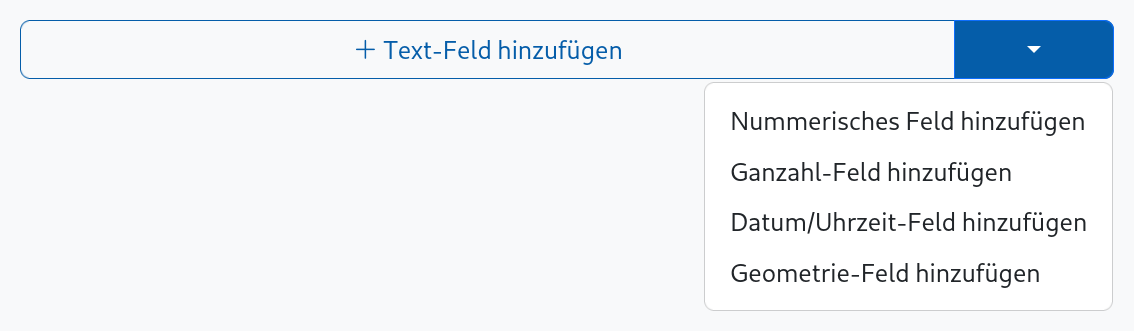
\includegraphics[width=.9\textwidth]{assets/datatype-dropdown.png}
  \caption{Dropdown zum Auswählen des Datentyps von Feldern im Szenario-Modus}
  \label{fig:type-dropdown}
\end{figure}

\plabel{p:ersetzen}
\todo[noline]{ZSMFG: Effizienz / gesparte Klicks}
In der Zielstruktur eingetragene Attribute können nicht ersetzt werden \textbf{(F)}. Dies fiel 4 Teilnehmer:innen auf. Sie versuchten, durch ein erneutes Anklicken eines bestehenden Eintrages den Inhalt mit einer Auswahl aus dem linken Menü zu überschreiben. Aktuell muss zuerst der Button zum Löschen gedrückt werden, wodurch das Feld wieder frei ist und erneut befüllt werden kann. Eine Person versuchte immer wieder eingetragene Attribute zu ersetzen, obwohl sie bereits festgestellt hatte, das dies nicht möglich ist. Zu beachten ist, dass ausschließlich versucht wurde, Attribute zu ersetzen, keine Funktionen. Dies könnte der Art und Weise geschuldet sein, wie eingetragene Attribute dargestellt sind - sie ähneln einem leeren Feld. In Abbildung \ref{fig:buffet-simple} ist der Unterschied zwischen einem leeren Feld, einer ausgewählten Funktion und einem ausgewählten Attribut zu sehen.
\todo{überprüfen ob das noch stimmt falls Bild ausgetauscht}

\plabel{p:drag}
Ebenso oft trat es auf, dass Teilnehmer:innen mittels \textit{Drag \& Drop} \textbf{(G)} Elemente von links nach rechts ziehen wollten. In jedem der 4 Fälle war es die erste Intuition und wurde ausgetestet. Nach der Realisation, dass \textit{Drag \& Drop} noch nicht implementiert ist, konnte der Großteil zur konzipierten Bedienweise übergehen. Dabei sollte zuerst das Zielfeld und dann das gewünschte Attribut, beziehungsweise die gewünschte Funktion, angeklickt werden. Andersrum \todo{wording} ist das ebenso möglich. Eine Person tat sich mit der Transition zu dieser Bedienweise schwer.

\plabel{p:parameterübernahme}
Beim Auswählen von Funktionsüberladungen werden die Parameter von einer Überladung nicht in die nächste übernommen \textbf{(H)}. Vier Personen waren davon verwirrt, dass die ersten, bereits ausgefüllten Parameter, leer sind, sobald eine Überladung mit mehr Parametern ausgewählt wird. Zwei von ihnen merkten an, dass die Anzahl der Parameter auch nach dem Ausfüllen anpassbar sein sollte, wobei eine von ihnen darauf einging dass es schwierig sein könnte, dies konsistent umzusetzen. Ein:e Teilnehmer:in erkannte, dass die zuvor eingetragenen Parameter in der Überladung mit weniger Parametern bestehen bleiben, und entfernte diese manuell, aus Angst dass dies Fehler verursachen könnte.

\begin{figure}[!h]
  \minipage[t]{.49\textwidth}
  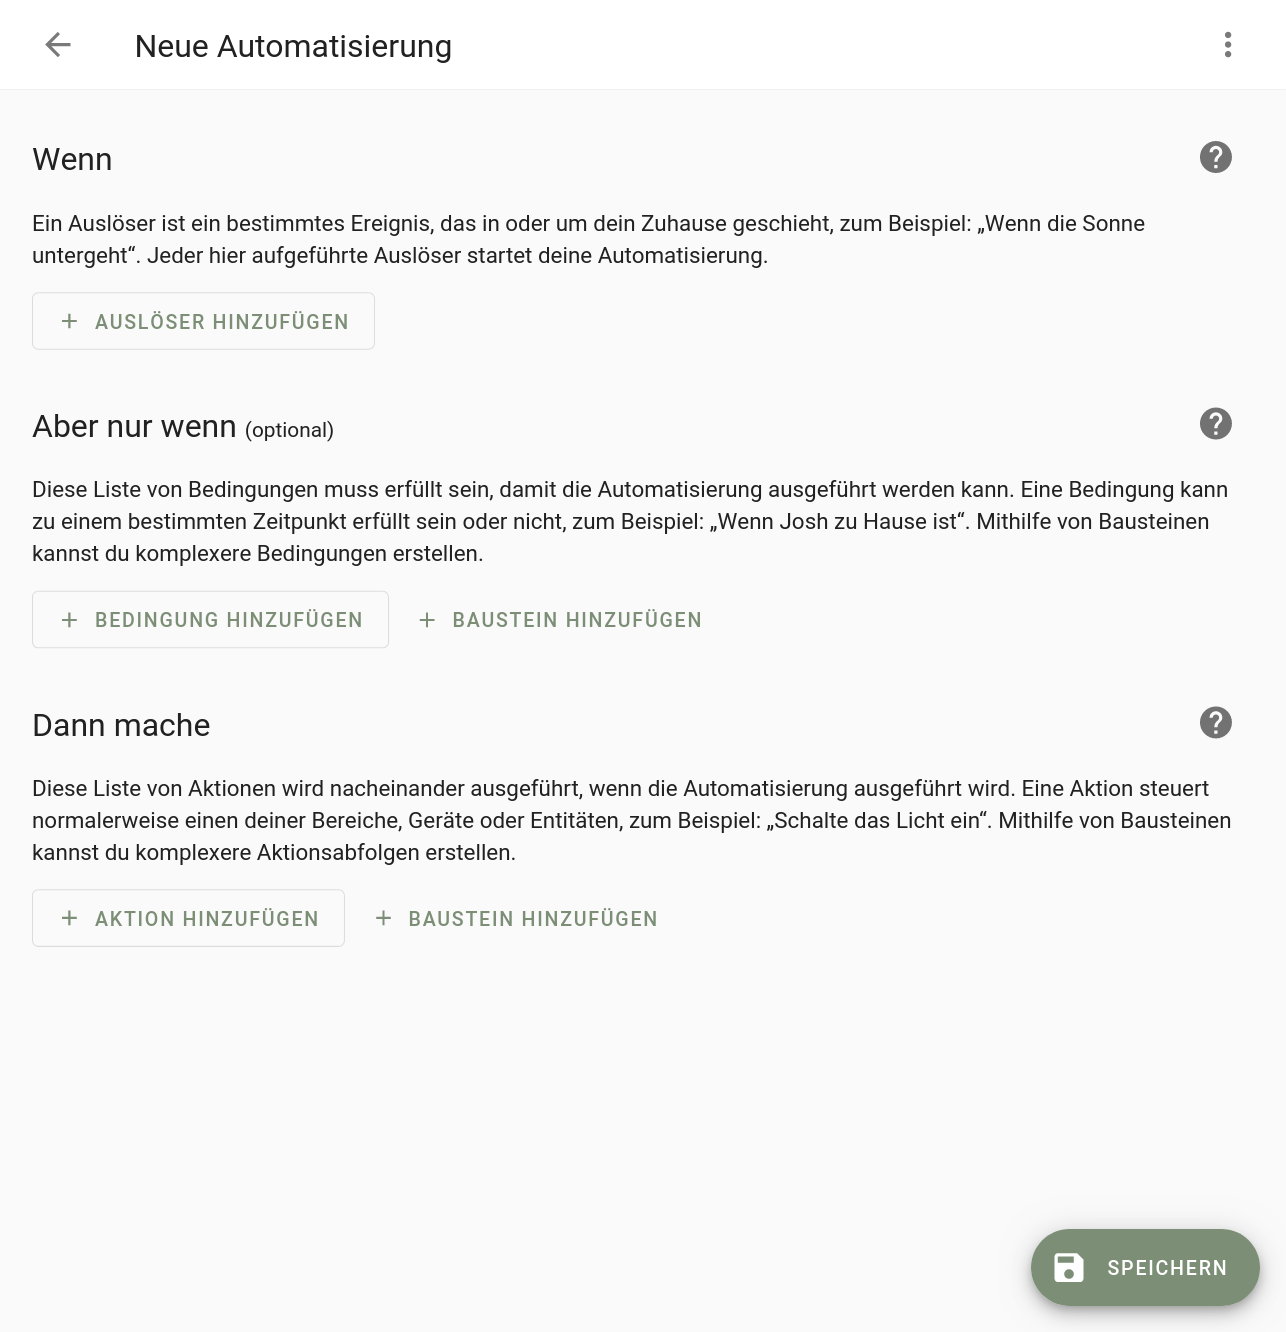
\includegraphics[width=\linewidth]{assets/hassio-automation-empty.png}
  \caption{Überladung der Funktion \texttt{concat} (4 Parameter).\todo{replace (tooltip)}}
  \label{fig:concat-overload}
  \endminipage
  \hfill
  \minipage[t]{.49\textwidth}
  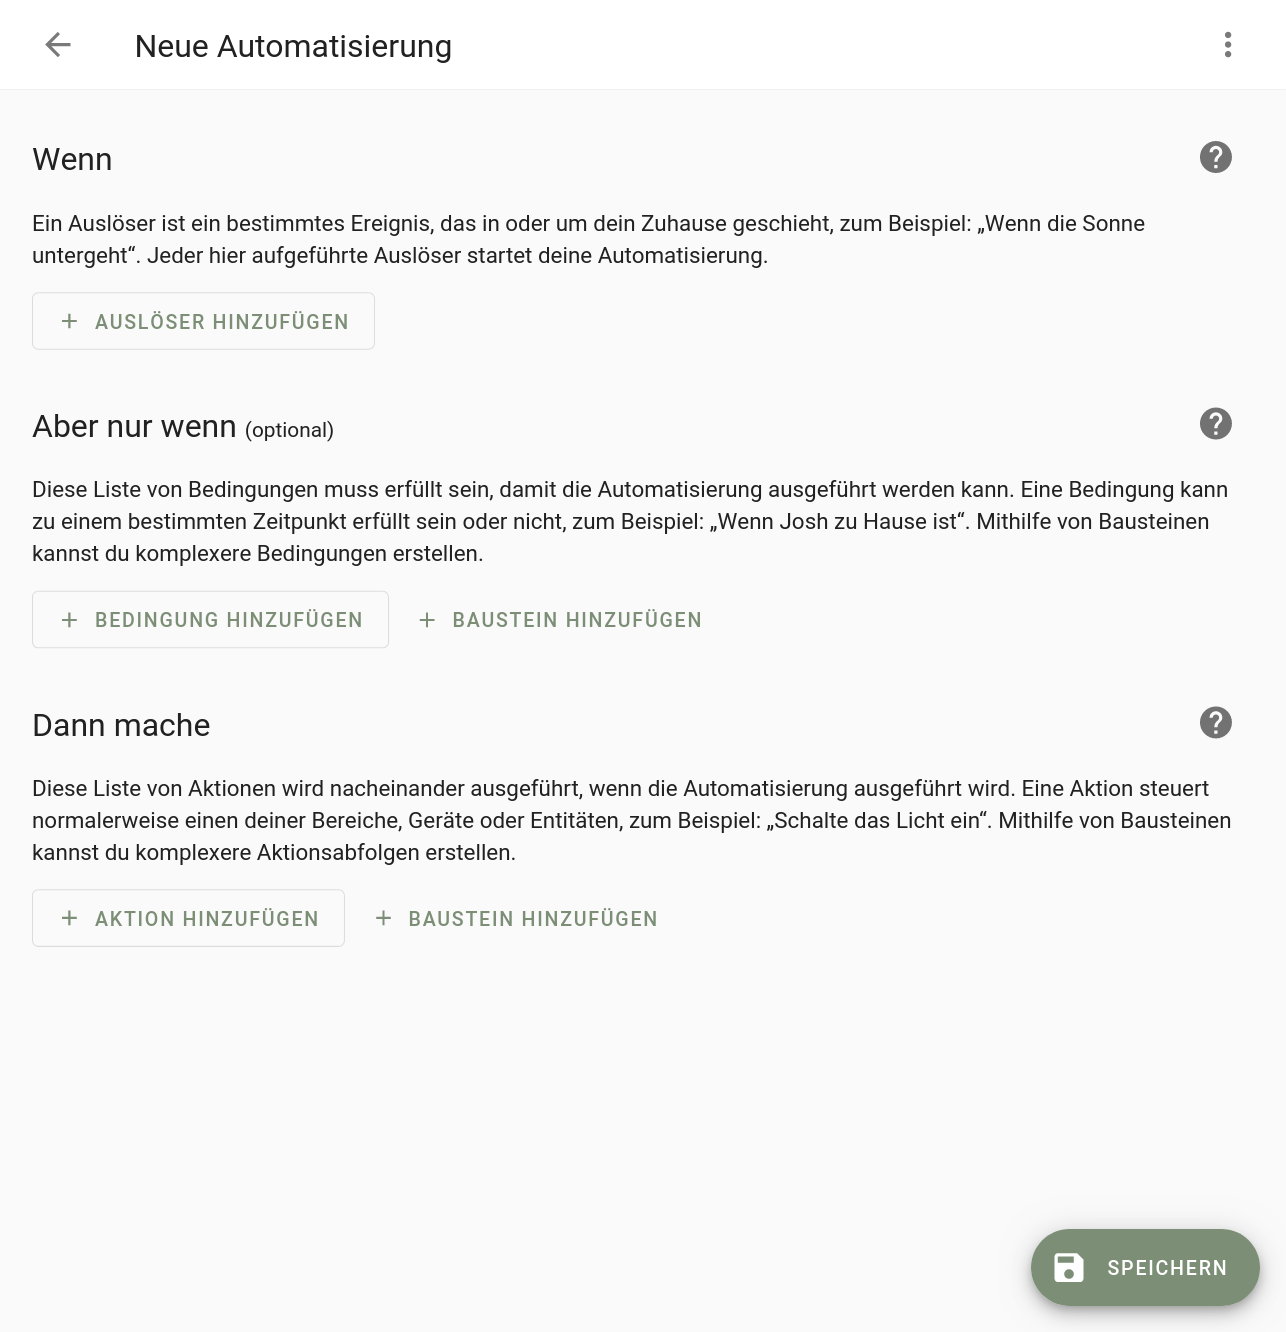
\includegraphics[width=\linewidth]{assets/hassio-automation-empty.png}
  \caption{Eine geschachtelte Version der Funktion \texttt{concat}.\todo{replace}}
  \label{fig:concat-nested}
  \endminipage
\end{figure}

\plabel{p:overload}
Von den Personen, die keine Probleme mit den Parametern von Überladungen hatten, benutzten 3 die Überladungs-Funktionalität gar nicht. Sie erkannten die Möglichkeit nicht, eine andere Überladung auszuwählen \textbf{(K)}. In Abbildung \ref{fig:concat-overload} und \ref{fig:concat-nested} ist die Funktion \texttt{concat} zu sehen, bei der es zu den genannten Problemen kam. Die 3 Personen, die keine Überladungen benutzten, wählten die in Abbildung \ref{fig:concat-nested} abgebildete Herangehensweise, die zur Folge hat, dass $n-1$ mal die Funktion ausgewählt werden muss, wobei $n$ die Anzahl der Einzelbestandteile ist. Zwei der drei Personen nahmen dies so hin, während die dritte es als "nervig" und "umständlich" bezeichnete. \todo{klingt das bisschen verletzt?} Im Nachhinein wies sie auch darauf hin, dass sie die Pfeile zum Umschalten zwischen Überladungen als ungeeignet errachtet. An dieser Stelle hätte sie eher ein Plus und Minus erwartet, oder vielleicht sogar ein Plus am Ende der Parameterliste platziert. In einer anderen Testsitzung wurde der in Abbildung \ref{fig:concat-overload} zu sehende Tooltip kritisiert, da die meisten Menschen nicht wissen, was Überladungen sind. \todo[noline]{ZSMFG: overload zu Anzahl parameter vereinfachen}

\plabel{p:statisch}
Die Angabe von statischen Werten \textbf{(L)} führte in 3 Testsitzungen zu 2 unterschiedlichen Problemen. Statische Werte können anstelle von Attributen oder Funktionen in Eingabefeldern eingegeben werden. Dabei kann der Wert ohne besonderen Syntax eingegeben werden, da es sich im Block-Editor um an den Datentyp angepasste Eingabefelder handelt. Eine Person war sah eine einfache Eingabe nicht als Option an und war sich nicht im Klaren dass dies möglich ist. Zwei weitere Teilnehmer:innen setzten ihre Texteingabe zunächst in Hochkommas, konnten diesen Fehler dann jedoch am Ende relativ schnell beheben. Die beiden zuletzt genannten Personen haben Programmier- und \ac{SQL}-Kenntnisse und nannten diese als Ursprung ihrer Handlung.

\plabel{p:filter}
Der Block-Editor filter automatisch relevante Auswahlmöglichkeiten basierend auf ihrem Datentyp \textbf{(O)}. In 3 Testsitzungen wurde diese Funktionalität missverstanden. Im extremsten Fall konnte die Testperson nichts mit den Datentypen anfangen, und war somit auch nicht in der Lage das Konzept des automatischen Typfilters zu verstehen. In einer anderen Testsitzung wurde zwar realisiert, dass beim Anklicken von Elementen links in der Zielstruktur Felder deaktiviert werden, dieser Effekt wurde allerdings dem falschen Grund zugeschrieben. Die Person war der Meinung, dass der Grund hierfür eine bereits getätigte Auswahl ist. In diesem Fall führte dies dazu, dass die durch die Filterung verursachten Änderungen in der UI äußerst untransparent wirkten. Auffällig war, dass alle 3 Teilnehmer:innen von links nach rechts arbeiteten, das heißt, es fiel ihnen schwerer den vollen Effekt der Filterfunktion zu verstehen. Eine dieser Personen äußerte sogar den Wunsch, die Liste der Funktionen zu filtern, erkannte aber nicht, wie dies funktioniert. Wenn die Oberfläche von rechts nach links benutzt wurde, trat dieses Problem nicht auf, es gab aber auch Teilnehmer:innen, die von von links nach rechts arbeiteten, und denen die Funktionsweise klar wurde. Eine:r von ihnen ging daraufhin sogar dazu über, zuerst das Feld rechts auszuwählen, und dann das einzufügende Element links rauszusuchen.

\subsubsection{Darstellungsprobleme}

Auch die Darstellung von Informationen innerhalb des Block-Editors führte zu Problemen. Es wurden 8 Darstellungsprobleme identifiziert, welche von unklaren Bezeichnungen bis hin zu Icons reichen.

\plabel{p:attribute}
\plabel{p:icons}
\plabel{p:speichern}
\plabel{p:mitte}
\plabel{p:meta}
\plabel{p:queryables}
\plabel{p:functionlist}

\subsubsection{Inhaltliche Probleme}

\plabel{p:parameter}
\plabel{p:quelle}
\plabel{p:functions}
\plabel{p:präfix}

\subsubsection{Technische Probleme}

\plabel{p:scroll}

\clearpage % TODO: check if needed
\subsection{Quantitative Auswertung}
\label{sec:quantitative}

Die Teilnehmer:innen wurden gebeten, sowohl die Einfachheit der Szenarios, als auch die Einfachheit der Benutzung des gesamten Block-Editors zu bewerten.

Ein Unterschied zwischen internen und externen Testpersonen konnte nur sehr begrenzt festgestellt werden. Das zweite Szenario wurde von Mitarbeiter:innen einfacher als von externen Testpersonen bewertet, wobei die meist größere \ac{SQL}- und Programmiererfahrung eine Rolle spielt. Die Vorversion des Block-Editors zur Bearbeitung von Konvertierungen wurde durch interne Testpersonen besser als von externen bewertet. Eine Ausnahme stellten Mitarbeiter:innen dar, die weniger Vorerfahrung mit dem Systemansatz haben. Die meisten Unterschiede zwischen den Einschätzungen der Testpersonen können auf unterschiedliche  Erfahrungsgrade zurückgeführt werden.

\subsubsection{Bewertung der Szenarios}

Im Anschluss an jedes Szenario wurde die \ac{SEQ} gestellt. Damit sollte überprüft werden, wie die Teilnehmer:innen die Schwierigkeit der einzelnen Aufgaben sehen und im Vergleich zueinander einschätzen. Es war explizit erwünscht, die drei Einschätzungen zueinander stimmig abzugeben. Die Frage wurden von allen Teilnehmer:innen beantwortet, das heißt für jedes Szenario wurden insgesamt 10 Werte erfragt. Abbildung \ref{fig:seq} zeigt die gesammelten Antworten für jedes Szenario, dargestellt als Box-Plot.

\begin{figure}[!ht]
  \pgfplotstableread[col sep=comma]{assets/study-results.csv}\datatable
  \centering
  \begin{tikzpicture}
    \begin{axis}[
        boxplot/draw direction=y,
        boxplot/every median/.style={ultra thick},
        xtick={1,2,3},
        xticklabels={Szenario 1, Szenario 2, Szenario 3},
        ytick={1,...,7},
        ymin=1,
        ylabel={\acl{SEQ}},
      ]
      \addplot+ [boxplot, plot1] table [y=a] {\datatable};
      \addplot+ [boxplot, plot2] table [y=b] {\datatable};
      \addplot+ [boxplot, plot3] table [y=c] {\datatable};
    \end{axis}
  \end{tikzpicture}
  \caption[Antworten auf die SEQ nach jedem Szenario]{Antworten auf die \acs{SEQ} nach jedem Szenario (1: sehr schwer, 7: sehr einfach). Gezeigt werden die Extremwerte (obere und untere Antenne), das obere und untere Quartil (Box) und der Median (dicke Linie).}
  \label{fig:seq}
\end{figure}

In allen Testsitzungen wurde das erste Szenario als am Einfachsten bewertet. Alle Teilnehmer:innen bewerteten es zwischen 5 und 7. Abzüge von Punkten wurde zumeist mit Startschwierigkeiten begründet, die sich im Laufe des ersten Szenarios gelöst haben. Nach einer initialen Einfindungsphase bestand die Aufgabe in diesem Szenario daraus, sich wiederholende Zuordnungen durchzuführen.

Das zweite Szenario wurde als etwas schwieriger bewertet, wobei sich die Gesamtheit der Bewertungen über einen größeren Bereich (3,5-7) verteilte. Die gesteigerte Komplexität in diesem Szenario kann  größtenteils auf die Verwendung von Funktionen zurückgeführt werden, dies wurde von einigen Teilnehmer:innen als Grund genannt. Personen, die das Szenario als schwieriger bewerteten, hatten in der Regel weniger \ac{SQL}- und Programmiererfahrung, während der Großteil der höheren Bewertungen von firmeninternen Testpersonen abgegeben wurde.

Die größte Streuung der Bewertungen kann im dritten Szenario beobachtet werden. Die angegebenen Werte liegen zwischen 3 und 7, wobei das untere und obere Quartil einen relativ großen Bereich abdeckt. Die unterschiedlichen Bewertungen und die Art der aufgetretenen Probleme zeigt, dass die Teilnehmer:innen variierende Erfahrungen während des letzten Szenarios gesammelt haben. Im Vergleich zum zweiten Szenario ist festzustellen, dass sich interne und externe Testpersonen im Wertebereich gleichmäßig verteilen. Vorwissen über Simplex4TwIS scheint einerseits weniger Wichtigkeit für ein erfolgreiches Abschließen des Szenarios zu haben, andererseits hatten Mitarbeiter:innen von Simplex4TwIS bisher nur wenige Möglichkeiten Szenarios zu erstellen (im Gegensatz zu Konvertierungen).

Indem in jedem Szenario mehr Funktionalitäten hinzugefügt wurden, sollte die Komplexität im Laufe einer Testsitzung steigen. Die Antworten auf die \ac{SEQ} bestätigen diese Erwartungshaltung nur begrenzt. Wie in Abbildung \ref{fig:seq} zu sehen, fielen die Angaben von Szenario 1 zu Szenario 2 im Median von 6 auf 5, stiegen jedoch im Szenario 3 wieder auf 6,5. Somit kann eine Komplexitätssteigerung zwischen den ersten beiden Szenarios festgestellt werden. Im dritten Szenario kann kein klarer Trend in eine der beiden Richtungen festgestellt werden, größtenteils bedingt durch die starke Streuung der Antworten.

\subsubsection{Bewertung des Block-Editors}

Abbildung \ref{fig:ges} zeigt die Einschätzung der Einfachheit der Benutzung der Anwendung, abgefragt am Ende der Testsitzungen. Während alle Teilnehmer:innen den Block-Editor bewerteten, konnten zwei Personen keine Aussage zur Vorversion treffen, da sie diese nie benutzt haben.

Die Teilnehmer:innen sagten aus, dass sie sich mit dem Block-Editor effizienter fühlen und die Bedienung durch Funktionalitäten wie die Typ-Filterung vereinfacht wird (Vgl. \ref{sec:qualitative}). Die Bewertungen bestätigen diese Aussagen.

\begin{figure}[!ht]
  \pgfplotstableread[col sep=comma]{assets/study-results.csv}\datatable
  \centering
  \begin{tikzpicture}
    \begin{axis}[
        boxplot/draw direction=y,
        boxplot/every median/.style={ultra thick},
        xtick={1,2},
        xticklabels={Vorversion, Block-Editor},
        ytick={1,...,10},
        ymin=1,
        ylabel={Einfachheit der Benutzung},
      ]
      \addplot+ [boxplot, plot1] table [y=prev] {\datatable};
      \addplot+ [boxplot, plot2] table [y=ges] {\datatable};
    \end{axis}
  \end{tikzpicture}
  \caption[Einschätzung der Einfachheit der Benutzung nach dem Usability Test]{Einschätzung der Einfachheit der Benutzung nach dem Usability
    Test auf einer Skala von 1 (sehr schwer) bis 10 (sehr einfach). Es wurde sowohl nach der Einfachheit der Benutzung des entwickelten Block-Editors, als auch der Vorversion gefragt.}
  \label{fig:ges}
\end{figure}

Kein:e Teilnehmer:in bewertete die Vorversion einfacher als den Block-Editor, alle Personen, die bereits zuvor Erfahrung mit dem existierenden System gesammelt hatten, konnten ein eindeutige Verbesserung der Einfachheit der Benutzung feststellen. Die Teilnehmer:innen waren sich einig, dass der Block-Editor eher einfach in der Benutzung ist, mit dem Großteil der Bewertungen über 8. Die schlechtesten Bewertungen für den Block-Editor wurden von Personen abgegeben, die wenig \ac{SQL}- und Programmiererfahrung besitzen, und Schwierigkeiten hatten, das Prinzip der Funktionen korrekt anzuwenden. Im Allgemeinen wurden die Abzüge von der Gesamtpunktzahl damit begründet, dass sich die Benutzer:innen zuerst in das Konzept des Block-Editors einfinden müssen, um produktiv zu sein, und dass ein gewisses Vorwissen von Nöten ist, um fachlich korrekte Abfragen zu erstellen.

Die Antworten bezüglich der Vorversion waren ein wenig gestreuter - den darauffolgenden Aussagen zufolge kann dies mit unterschiedlichen Erfahrungsgraden begründet werden. Die höchsten Bewertungen für die Vorversion wurden von internen Testpersonen getätigt, die äußerst vertraut mit der Funktionsweise von Simplex4TwIS sind und dies auch selbst zu ihrer Bewertung aussagten. Teilnehmer:innen mit weniger Erfahrung bewerteten die Vorversion hingegen als schwerer. Als Gründe für die niedrigere Benutzbarkeit der Vorversion wurde Umständlichkeit, Fehleranfälligkeit und die fehlende Sicht auf die Quelldaten genannt.


\cleardoublepage
\section{Schlussfolgerungen und Zukunftsaussicht}

Die Usability-Studie des Prototyps hat gezeigt, dass die allgemeine Herangehensweise gut angenommen wurde. Tippfehler wurden verhindert, und ein Nachschlagen der Quellstrukturen während dem Abarbeitung von Aufgaben war nicht nötig. Je nach technischer Vorkenntnis und Vertrautheit mit dem System Simplex4TwIS konnten die Teilnehmer:innen schnell mit dem Block-Editor arbeiten und die gewünschten Resultate erzielen. Die getestete Anwendung erweist sich somit in den getesteten Anwendungsfällen als geeignet zur Bearbeitung von Umweltdatensätzen.

Zur Anwendung in der Praxis und für die Integration in das Produktiv-System Simplex4TwIS muss jedoch ein umfangreicherer Katalog an Funktionen unterstützt werden. Das Hinzufügen dieser Funktionen kann im Backend durchgeführt werden, ohne den Editor anzupassen, da die Kommunikation zwischen den beiden Schichten über die standardisierte \textit{OGC - API Features} Schnittstelle realisiert wird. Diesbezüglich steht allerdings die Frage aus, ob die aktuelle Herangehensweise zum Erstellen von Konvertierungen und SimplexSzenarios ausreicht, oder der Komplexität der Praxis nicht gerecht wird. In diesem Fall bestünde einerseits die Möglichkeit, eine komplexere Anwendung zur Bedienung durch Expert:innen zu erstellen. Andererseits könnten Prä- oder Postprozesse müssen zur Datentransformation eingesetzt werden, um die Daten in ein Format zu überführen, welches im Block-Editor und von Fachanwender:innen benutzt werden kann.

Die durchgeführten Usability-Tests führten dazu, dass verschiedene Hürden aufgedeckt wurden, die die Einfachheit der Nutzung einschränken. Während einige von ihnen bereits im Vorhinein bekannt waren, wurden viele neue im Zuge der Testsitzungen dokumentiert. Dabei unterscheiden sich die aufgetretenen Probleme in Größe und Härte. Einige von ihnen können schnell gelöst werden, während andere Fragen aufwerfen, die noch beantwortet werden müssen. Des Öfteren haben auch Teilnehmer:innen bereits Verbesserungsvorschläge geäußert, die im Folgenden auch diskutiert werden sollen. Abschnitt \ref{sec:criticism} nennt bereits einige Schritten zur Weiterentwicklung für den Block-Editor. Insofern diese keine große Rolle während den Usability-Tests gespielt haben, werden diese hier nicht erneut aufgegriffen.

% - Allgemeine Schlussfolgerungen
%   - wurde gut angenommen blabla schreibfehler nachschlagen etc.
%   - für die getesteten anwendungsfälle, in der Praxis müssen Funktionen hinzugefügt werden - sollte einfach hinzuzufügen sein, da standardisiertes interface - aber reicht das für anwendungsaufgaben aus? Da Komplexität in der Praxis nicht voraussehbar ist, müssen Wege geschaffen werden, um komplexe Abfragen zu ermöglichen - expert:innen Ansicht

\subsubsection{Schnell zu behebende Probleme}

Oft gewünscht wurde die Möglichkeit, Elemente durch Klicken zu ersetzen. Dazu müssten ausgefüllte Felder anklickbar bleiben. So wird einerseits ein Klick gespart, andererseits wurde dieses Bedienschema von einigen Teilnehmer:innen als intuitiver wahrgenommen. Die aktuelle Möglichkeit, über einen dedizierten Button den Inhalt eines Felds zu löschen, sollte jedoch weiterhin erhalten bleiben.

Um die Einfindung in der Bearbeitungsoberfläche zu erleichtern, können relevante Bereiche besser benannt werden. Die Benennung der "Abfragbaren Felder" könnte verbessert werden. Im Konvertierungs-Editor würden sie als "Importtabelle" bezeichnet werden, und im Szenario-Editor als "(Objekt-)Attribute". Somit würden der Inhalt klarer beschrieben werden. Des Weiteren sollte der rechte Bereich mit einer Überschrift benannt werden, sodass klar ist, was bearbeitet wird. Auch die Überschrift der Anwendung in der Kopfzeile sollte mit dieser Zielsetzung angepasst werden.

Ein weiteres Problem der Darstellung trat bei der Anzeige der abfragbaren Felder in der Zielstruktur auf. Dort wurde nur der Schlüssel des Attributs (oder Importtabellenspalte) angezeigt, obwohl im Auswahlmenü der Titel prominenter dargestellt wurde. In der nächsten Version des Editors sollte dies vereinheitlicht werden, wobei zu beachten ist, dass die abfragbaren Felder nicht unbedingt über einen Titel verfügen. Es kann also entweder wenn möglich beides angezeigt werden, oder falls verfügbar der Titel, sonst der Schlüssel.

Im Szenario-Editor besaß die zentrale Klasse kein Präfix, um die Verständlichkeit zu verbessern sollte dies nicht der Fall sein. Der Präfix bietet einen Weg, um Elemente eindeutig einer Klasse zuzuordnen, diese Möglichkeit sollte einheitlich genutzt werden. Zur Umsetzung müssen Änderungen am Szenario-Join-Editor und an der \texttt{queryables}-Schnittstelle vorgenommen werden, damit ein Präfix vergeben werden, von der \ac{API} ausgegeben und im Szenario-Editor angezeigt werden kann.

Während mehreren Testsitzungen wurde klar, dass die Icons für die Datentypen Boolean, Integer und Float etwas unglücklich gewählt sind (siehe Abbildung \ref{fig:icons}). Booleans wurden als Schaltfläche verstanden, während Integers und Floats nicht voneinander zu unterscheiden waren. Die Wahl der Icons sollte in der nächsten Version der Anwendung verändert werden.

Überprüft werden sollte das Scroll-Verhalten in verschiedenen Browsern, um visuelle Fehler zu vermeiden. Außerdem sollte überprüft werden, ob der Abstand zum Seitenende groß genug ist, denn zwei Personen hätten gerne ein wenig weiter gescrollt. Im gleichen Zusammenhang kann getestet werden, ob es Sinn ergibt automatisch zu scrollen, wenn eine neue Funktion hinzugefügt wird die nicht komplett im Ansichtsfenster dargestellt wird. Unnötiges, nicht von Nutzer:innen ausgelöstes, Scrollen sollte jedoch vermieden werden.


% - schnell zu behebende Fehler
%   - Ersetzen von Items durch einfaches Klicken (4)
%   - benennung mitte und abfragbaren felder
%   - anzeige von attributen im ziel vereinheitlichen
%   - präfix von objektklassen
%   - scrolling
%   - icons für booleans und float verbessern

\subsubsection{Verbesserungsvorschläge von Teilnehmer:innen}

Im Zuge der Testsitzungen äußerten einige Teilnehmer:innen bereits Verbesserungsvorschläge. Einige von ihnen, die einfach umzusetzen und logische nächste Schritte darstellen wurde bereits im vorherigen Abschnitt genannt\footnote{Ersetzen, verbesserte Benennungen}. Im Folgenden werden weitere Vorschläge präsentiert und diskutiert.

Die Bearbeitungsfunktion für Titel und Schlüssel von Feldern im Szenario-Editor wurde nicht immer genutzt. Der Unterschied zwischen den beiden Metadaten-Feldern war einigen Personen nicht sofort klar, und zwei Personen drückten Unzufriedenheit damit aus, dass sie meistens den gleichen oder ähnlichen Text in die Felder schreiben müssen. Sie schlugen vor, den Schlüssel automatisch mit einer \texttt{slugify}-Funktion zu generieren, sobald sich der Titel ändert. Dieser Vorschlag ist sinnvoll, bei der Implementierung muss jedoch darauf geachtet werden, dass der Schlüssel weiterhin eindeutig bleibt und manuell angepasst werden kann.

Mit der Verbesserung der Effizienz im Szenario-Editor befasst sich ein weiterer Vorschlag. Neu hinzugefügte Felder könnten sofort ausgewählt werden, nachdem sie hinzugefügt wurden, wodurch ein Klick eingespart wird und das Auswahlmenü sofort auf die richtigen Elemente reduziert wird. Eine Umsetzung dieser Funktionalität könnte die Benutzung beschleunigen, sollte jedoch gut überlegt sein. In einigen Usability-Tests war zu sehen, dass die automatische Typ-Filterung nicht sofort verstanden und eingesetzt wurde. Außerdem bevorzugten einige Teilnehmer:innen, zuerst das Element im Auswahlmenü auszusuchen, und dann in das gewünschte Zielfeld zu klicken. Eine automatische Auswahl nach Hinzufügen des Elementes könnte dieser Arbeitsweise beeinträchtigen oder zu Verwirrung führen.

Ein:e Teilnehmer:in empfand die Liste der Funktionen als zu unübersichtlich, und schlug vor, Unterkategorien einzuführen. Da die Anzahl der Funktionen im Vergleich zum getesteten Prototyp weiter steigen wird, könnte dies sinnvoll sein. Sobald eine angemessene Anzahl an Funktionen existiert, sollte überprüft werden, ob der automatische Typ-Filter genug Übersichtlichkeit schafft, oder ob und wie die Funktionen weiter gruppiert werden können.

Ein bereits während der Entwicklung aufgetretener Vorschlag beinhaltete, Die ausgefüllten Zielfelder mit ihren Bestandteilen aus dem Auswahlmenü über eine Linie oder einen Pfeil zu verbinden. In einer Testsitzung wurde dieser Wunsch erneut geäußert, da die Person dieses Konzept aus anderen Anwendungen kennt. Eine Umsetzung könnte Übersichtlichkeit über die definierten Strukturen schaffen, und Fehler wie doppelte Selektionen vermeiden. Es sollte jedoch getestet werden, wie sich eine solche Ansicht bei vielen Elementen verhält. Es wäre denkbar, die Verbindungsstriche als optionales UI-Element zu implementieren.

Häufig gefordert wurde auch die Möglichkeit eine Stichprobe der Daten, die bearbeitet werden, zu sehen. Bevor diese sinnvolle Erweiterung umgesetzt werden kann, muss geklärt werden, wo die Daten angezeigt werden sollen, und in welchem Umfang dies geschehen soll. Es wäre möglich, Werte für einzelne abfragbare Felder bereitzustellen, oder einen Querschnitt über alle abfragbaren Felder eines Datensatzes. Optimalerweise würde das Abrufen der Daten nicht dazu führen, dass Nutzer:innen den aktuellen Browser-Tab verlassen müssen.

Die Auswahlmöglichkeit von Funktionsüberladungen wurde nicht immer erkannt, als Grund dafür wurden mehrfach die Icons auf den dazugehörigen Buttons genannt. Statt der aktuell genutzten Pfeile wurde vorgeschlagen, ein Plus und Minus zu verwenden. Da den wenigsten Teilnehmer:innen das Konzept von Funktionsüberladungen geläufig war, und viele von ihnen diese nur als Möglichkeit ansahen, die Anzahl der Parameter zu verändern, ergibt es Sinn die Icons so anzupassen. Im gleichen Schritt muss jedoch geklärt werden, wie mit Funktionsüberladungen mit der gleichen Anzahl an Parametern, aber unterschiedlichen Typen umgegangen wird. Eine Möglichkeit wäre, Felder mit mehreren akzeptierten Typen einzuführen, wodurch jede Überladung eine unterschiedliche Anzahl an Parametern haben könnte.

Die Benutzung der Funktionen wurde teilweise dadurch erschwert, dass die Parameter nicht über genügend Metadaten verfügten. Es war nicht immer möglich, eindeutig zu erkennen, welcher Parameter welche Information entgegennimmt, wie im Beispiel der Funktion \texttt{ST\_MakePoint}. Die einzelnen Parameter sollten somit zumindest über Namen verfügen. Die \textit{OGC API - Features}-Schnittstelle für Funktionen unterstützt bereits die Metadaten-Felder \texttt{title} und \texttt{description}, diese müssen im Backend hinzugefügt werden und durch den Block-Editor ausgelesen und angezeigt werden. Der Großteil der Teilnehmer:innen erwartet diese Informationen direkt beim dazugehörigen Eingabefeld. Eine Beschreibung einzelner Parameter könnte hinter einem Info-Button versteckt sein, um die Ansicht nicht mit Informationen zu überladen. Nicht alle Funktionen sind so komplex, dass die Parameter über Namen, geschweige denn Beschreibungen verfügen müssen. Für alle drei Optionen sollte die Art und Weise, wie Parameter dargestellt werden, angepasst werden.

% - Verbesserungsvorschläge von Teilnehmer:innen
%   - notfalls einschätzen falls nicht sinnvoll
%   - szenario: slugified key von titel abgeleitet (J, V; 2)
%   - szenario: automatisch bei neu hinzugefügten feldern reinklicken? spart einen klick (heino; 1)
%   - übersichtlichkeit funktionsliste
%   - pfeil von links nach rechts (würde auch auswahlfehler verhindern)
%   - stichprobe von daten, offene Fragen: wo? in welchem Umfang?
  % - Overload Funktionalität vereinfachen, viele kennen overloads nicht - anzahl der parameter schon
%   - parameter metadaten, beschreibung z.b. längen und breitengrad
%     - muss von backend unterstützt werden, dort müssen metadaten hinzugefügt werden - dann im frontend anzeigen
%     - wird schon von ogc unterstützt, parameter können title und description haben
%     - funktion kann metadataUrl haben, die nicht weiter dokumentiert ist (zitat) aber für hilfestellung für fkt benutzt werden könnte

\subsubsection{Weitere Möglichkeiten zur Verbesserung}

Aufgefallen ist, dass die Arbeitsrichtung zwischen den Teilnehmer:innen schwankte. Viele von Ihnen bedienten den Block-Editor von rechts nach links, indem sie zuerst das Zielfeld auswählten und dann das gewünschte Element einfügten. Es gab jedoch auch Personen, die andersherum vorgingen. Der aktuelle Prototyp unterstützt beide Richtungen, unterstützt die Nutzer:innen jedoch durch die automatische Typ-Filterung besser, wenn sie von rechts nach links arbeiten. Um diese Diskrepanz zu verringern, können zwei Wege eingeschlagen. Entweder werden beide Arbeitsweisen auf ähnliche Art und Weise unterstützt, sodass weniger Benachteiligung entsteht, oder die Bedienweise von Links nach Rechts wird unterbunden. Letzteres könnte dadurch umgesetzt werden, dass das Auswahlmenü erst nach Anklicken eines Zielfeldes angezeigt wird, oder vorher nicht anklickbar, aber sichtbar ist. Eine weitere Möglichkeit wäre, das Auswahlmenü auf der rechten Seite zu platzieren, sodass die Arbeitsrichtung mehr mit der hierzulande genutzten Leserichtung übereinstimmt. Dies könnte bei beiden Optionen sinnvoll sein. Mit der Entscheidung der Arbeitsweise verbunden ist die Frage, ob \textit{Drag \& Drop} implementiert werden sollte, da dies nur beim Ziehen der Quellelemente in die Zielstruktur sinnvoll ist.

Das Auswählen der Datentypen im Szenario-Editor ist aktuell zu umständlich. Theoretisch wäre es möglich, den Datentyp der Felder basierend auf dem Inhalt ihrer Definition zu bestimmen. Es könnte ein Eingabefeld eingeführt werden, in das alle Datentypen eingefügt werden können. Dies führt zwar dazu, dass die als nervig empfundene Typ-Auswahl entfällt, hat jedoch auch zur Folge, dass die Nutzer:innen nicht durch die automatische Typ-Filterung unterstützt werden.

% - weiter einzuschlagende Schritte, die nicht von Teilnehmer:innen erwähnt wurden
%   - LtR workflow verbessern, da dies von einigen als intuitiv angesehen wurde, oder RtL workflow forcen
%     - vielleicht wäre es möglich das menü links gar nicht immer zu zeigen, nur bei auswahl? so geht nur RtL
%     - damit verbunden wäre die frage ob dragndrop unterstützt werden sollte, weil das nur bei ltr geht
%   - verbesserung könnte auch bei szenario feldern benutzt werden (alle typen gehen rein), typ steht nicht vorher fest - auswahl fällt weg, die zuvor nervig war

\subsubsection{Offene Fragen}

Die folgenden Fragen wurden im Laufe der Usability-Studie aufgeworfen, konnten aber noch nicht auf zufriedenstellende Art beantwortet werden. Um ein optimales Nutzungserlebnis zu ermöglichen, sollten sie jedoch überdacht werden.

Einige Operatoren, die typischerweise durch Infixnotation ausgedrückt werden (\texttt{+}, \texttt{-}, \texttt{||}, \texttt{AND}, \texttt{OR}), werden im Block-Editor über Funktionen abgebildet. Bereits bei der Verwendung der \texttt{concat}-Funktion suchten mehrere Teilnehmer:innen nach einem \texttt{+} oder versuchten, zuerst das erste Element, und dann den dazugehörigen Operator in das Zielfeld einzufügen. Zwar ist es möglich, Infix-Operatoren über Funktionen darzustellen, dies scheint jedoch mitunter als nicht intuitiv aufgefasst zu werden und erschwert die Verkettung von mehreren Elementen. Die Anzahl der Parameter kann zwar über Funktionsüberladungen erhöht werden, entspricht aber nicht dem gleichen Nutzungserlebnis von Verkettungen mit Infix-Operatoren. Es ist zu diskutieren, ob mit Operatoren anders umgegangen werden sollte als mit Funktionen, und ob dafür eigene UI-Elemente und -Verhaltensmuster geschaffen werden sollten.

Eine Hürde bei der Benutzung von Funktionsüberladungen bestand darin, dass bereits ausgefüllte Parameter nicht übernommen wurden. Wie eine Übernahme von Parametern in andere Funktionsüberladungen auch in Randfällen vorhersehbar durchgeführt werden kann ist noch ungeklärt. Solche Randfälle beinhalten beispielsweise die Veränderung des Datentyps von Parametern, die Veränderung der Bedeutung von Parametern, sowie ein Wegfallen von bereits ausgefüllten Parametern.

Das eben genannte Problem könnte teilweise durch Felder mit variablen Datentypen (begrenzt auf die möglichen Datentypen für einen Parameter in Funktionen) gelöst werden. Dies birgt jedoch weitere Probleme in sich, da so die Möglichkeit besteht, ausgeschlossene Kombinationen von Datentypen zu ermöglichen, die zuvor durch Überladungen voneinander ausgeschlossen wurden. Eine dynamische Anpassung der validen Datentypen für einzelne Parameter könnte sehr komplex werden, eine Fehlermeldung beim Eintragen oder Abschicken wäre jedoch auch nicht optimal.

% - offene Fragen:
%   - wie wird mit Operatoren umgegangen die typischerweise infix sind (z.B. +)
%     - normale bedienweise wäre da erst paramter 1 dann operator dann parameter 2 auswählen, würde aber über api als funktion abgebildet werden
%     - funktional ähnlich, auch wenn aneinanderkettung schwieriger ist - parameter anzahl könnte bei funktionsdarstellung erhöht werden, aber das ist dann auch limitierend
%   - welche heuristik wird bei der Parameterübernahme bei Überladungen genutzt werden? 
%     - Frage: wie wird mit unterschiedlichen typen bei gleicher anzahl umgegangen?
%   - Antwort: typen sollten variabel sein für einzelne Parameter - vereinfacht das
%     - Frage: wie wird mit ausgeschlossenen Kombinationen umgegangen? Fehlermeldung beim Eintragen/Abschicken oder dynamisches Anpassen des Types sobald ein anderer ausgewählt wurde? könnte sehr komplex werden


\chapter{Fazit}

%
% Anhang
%

\appendix
\part*{Anhang}
\markboth{}{}
\addcontentsline{toc}{part}{Anhang}

\ifdefined\STANDALONE
  \section*{Einladung zur Usability-Studie}
\else
  \chapter{Einladung zur Usability-Studie}
\fi

\begin{tabular}{ l l }
  \textbf{Zeitaufwand} & 45 Minuten                                                                   \\
  \textbf{Ort}         & Online-Konferenzraum von Simplex4Data                                        \\
  \textbf{Termin}      & flexibel nach Absprache, jeder Wochentag möglich                             \\
  \textbf{Kontakt}     & \href{mailto:joshua.jeschek@simplex4data.de}{joshua.jeschek@simplex4data.de}
\end{tabular}

\vspace{2\baselineskip}

\noindent
Im Rahmen meiner Bachelorarbeit arbeite ich an der Entwicklung einer Low-Code Anwendung, die das
System Simplex4Data erweitern soll. Diese Anwendung zielt darauf ab, die Konvertierung und
Bearbeitung von Datensätzen durch einen blockbasierten Ansatz zu vereinfachen. Dabei soll ein
Tool erschafft werden, welches effiziente und benutzerfreundliche Datenbearbeitung für Fachleute
ermöglicht - unabhängig davon, ob sie bereits Erfahrung mit dem Simplex-Ansatz und Datenbanken haben
oder nicht.

Für die Weiterentwicklung und Optimierung dieses Projekts bin ich auf der Suche nach Fachleuten,
die im Arbeitsalltag mit (Geo)-Datensätzen umgehen. Ein tiefgehendes Verständnis von Datenbanken ist
für die Teilnahme an diesem Projekt nicht erforderlich. Ihr Fachwissen und Ihre praktischen
Erfahrungen sind von unschätzbarem Wert, um die Anwendung so zu gestalten, dass sie den realen
Anforderungen und Herausforderungen in der Praxis gerecht wird.

Um dies zu erreichen, plane ich, eine qualitative Studie durchzuführen, bei der Sie die Möglichkeit
haben, die Anwendung in einer Videokonferenz und über Bildschirmfreigabe auszutesten. Dabei
werden praxisnahe Problemstellungen bearbeitet, um ein tiefgehendes Verständnis für die
Funktionsweise und den Nutzen der Anwendung zu entwickeln. Dies bietet auch die Gelegenheit,
eventuelle Fehler zu identifizieren und durch Ihr Feedback und Ihre Verbesserungsvorschläge
direkt zur Weiterentwicklung der Anwendung beizutragen.

Mit Ihrer Teilnahme können Sie die Entwicklung der Anwendung beeinflussen, und somit dafür sorgen
dass es einfacher zu benutzen ist und den Anforderungen der Realität gerechnet wird.

Für weitere Informationen und bei Interesse an einer Teilnahme kontaktieren Sie mich bitte unter
\texttt{\href{mailto:joshua.jeschek@simplex4data.de}{joshua.jeschek@simplex4data.de}}. Ich freue mich auf
ihre Teilnahme und Feedback, um gemeinsam die Anwendung zu verbessern und auf Ihre Bedürfnisse
abzustimmen.

\begin{flushright}
  Joshua Jeschek

  Simplex4Data GmbH

  März 2024
\end{flushright}

\ifdefined\STANDALONE\else
  \chapter{Handout Usability Studie}
  \label{app:handout}
\fi

\subsection*{Szenario 1: Import von Bundesländern}
\href[pdfnewwindow=true]{https://db01.simplex4data.de:444/develop/joshua/cql/?functions=/develop/joshua/simplexservice/functions&queryables=/develop/joshua/simplexservice/scenarios/1/collections/14-1-103/queryables&output_class=/develop/joshua/simplexservice/scenarios/1/collections/14-1-104/queryables}{Startpunkt Szenario 1}

\vspace{\baselineskip}\noindent
Gegeben ist eine Importtabelle mit Daten zu den Bundesländern. Sie wollen diese in das Simplex4Data
System importieren. Dazu existiert bereits eine Objektklasse mit den nötigen Attributen.

\vspace{\baselineskip}\noindent
Die Importtabelle sieht in etwa so aus:

\begin{flushleft}
  \begin{tabular}{||c | c | c | c | c | c | c | c | c ||}
    \hline
    bezeichnung & name      & ars    & nuts   & nbd    & ibz    & bemerkung & wirksamkeit & geom       \\ [0.5ex]
    \hline\hline
    'Freistaat' & 'Sachsen' & '14'   & 'DED'  & 'ja'   & 20     & '--'      & 2014-02-01  & <geometry> \\
    \hline
    \vdots      & \vdots    & \vdots & \vdots & \vdots & \vdots & \vdots    & \vdots      & \vdots     \\
    \hline
  \end{tabular}
\end{flushleft}

\vspace{\baselineskip}\noindent
Die Objektklasse enthält folgende Attribute:
\begin{flushleft}
  \begin{tabular}{ || l || }
    \hline
    Bundesland            \\
    \hline
    key - ARS             \\
    typ - Bezeichnung     \\
    title - Name          \\
    cmt - Bemerkung       \\
    beg - Wirksamkeit     \\
    nuts - NUTS           \\
    nbd - NBD             \\
    ibz - IBZ             \\
    fl - Flächengeometrie \\
    \hline
  \end{tabular}
\end{flushleft}

\vspace{\baselineskip}\noindent
Weisen Sie die Daten aus der Importtabelle den korrespondierenden Attributen aus der Objektklasse
zu, und überprüfen Sie das Resultat.

\clearpage

\subsection*{Szenario 2: Import von Gemeinden}
\href[pdfnewwindow=true]{https://db01.simplex4data.de:444/develop/joshua/cql/?functions=/develop/joshua/simplexservice/functions&queryables=/develop/joshua/simplexservice/scenarios/1/collections/14-1-100/queryables&output_class=/develop/joshua/simplexservice/scenarios/1/collections/14-1-105/queryables&filter=on}{Startpunkt Szenario 2}

\vspace{\baselineskip}\noindent
Analog zu den Bundesländern sollen Gemeinden importiert werden. Die Daten in der Quelltabelle liegen
nicht einfach zur Zuordnung bereit, sondern müssen teilweise umgeformt werden.

\noindent Die Quelltabelle enthält auch Einträge, die sich nicht auf Gemeinden beziehen. Diese
können daran erkannt werden, dass \texttt{gemeinde\_id} nicht angegeben ist, und sollen nicht
importiert werden.

\vspace{\baselineskip}\noindent
Hier ein Auszug aus der Quelltabelle:
\begin{flushleft}
  \begin{tabular}{|| c | c | c | c | c | c | c | c ||}
    \hline
    gemeindename  & breitengrad & \dots  & bevoelkerung & flaeche & gemeinde\_id & \dots  & land\_id \\ [0.5ex]
    \hline\hline
    'Saarbrücken' & 49.236608   & \dots  & 179634       & 167.52  & '10'         & \dots  & '10'     \\
    \hline
    \vdots        & \vdots      & \vdots & \vdots       & \vdots  & \vdots       & \vdots & \vdots   \\
    \hline
  \end{tabular}
\end{flushleft}

\vspace{\baselineskip}\noindent
Die Objektklasse enthält folgende Attribute:
\begin{flushleft}
  \begin{tabular}{ || l || }
    \hline
    Gemeinde                                        \\
    \hline
    title - Name                                    \\
    key - ARS                                       \\
    bevoelkerung\_je\_km2 - Bevölkerung je km2      \\
    bevoelkerung\_weiblich - Bevölkerung weiblich   \\
    bevoelkerung\_männlich - Bevölkerung männlich   \\
    bevoelkerung\_insgesamt - Bevölkerung insgesamt \\
    flaeche\_km2 - Fläche in km2                    \\
    pt - Punktgeometrie                             \\
    \hline
  \end{tabular}
\end{flushleft}

\vspace{\baselineskip}\noindent
Der ARS (Amtlicher Regionalschlüssel) setzt sich wie folgt zusammen:
\[
  \underbrace{\scalebox{3}{10}}_{\texttt{land\_id}}\overbrace{\scalebox{3}{0}}^{\texttt{bezirk\_id}}\underbrace{\scalebox{3}{41}}_{\texttt{kreis\_id}}\overbrace{\scalebox{3}{0100}}^{\texttt{verband\_id}}\underbrace{\scalebox{3}{10}}_{\texttt{gemeinde\_id}}
\]

\clearpage

\subsection*{Szenario 3: Auflistung der Adressen in einem Leipziger Ortsteil}
\href[pdfnewwindow=true]{https://db01.simplex4data.de:444/develop/joshua/cql/?functions=/develop/joshua/simplexservice/functions&queryables=/develop/joshua/simplexservice/scenarios/1/collections/1-1-119/queryables?joins=%3E1-1-119:1-3-121-obj-0:nn,%3C1-3-121-obj-0:1-1-108-obj-strasse,%3E1-1-119:1-3-120-obj-1:nn,%3C1-3-120-obj-1:1-1-103-obj-ortsteil&filter=on}{Startpunkt Szenario 3}

\vspace{\baselineskip}\noindent
In diesem Szenario sind die Objektklassen bereits importiert. Dabei handelt es sich um:
\begin{itemize}
  \item Adressen (Hausnummer, PLZ, Geometrie)
  \item Straßen (Straßenname)
  \item Ortsteile (Ortsteil-Name)
\end{itemize}

\vspace{\baselineskip}\noindent
Die Klassen sind miteinander verknüpft und sollen nun zu einer Übersicht aller Adressen \textbf{im Ortsteil
  "Lindenau"} zusammengestellt werden.

\vspace{\baselineskip}\noindent
Die Liste sollte am Ende folgende Informationen enthalten:
\begin{itemize}
  \item Straßenname
  \item Hausnummer
  \item Adresszusatz
  \item Postleitzahl
  \item Ortsteil-Name
  \item Punktgeometrie(n)
\end{itemize}

\ifdefined\STANDALONE
  \section*{Skript für Moderation der Usability-Studie}
\else
  \chapter{Skript für die Moderation der Usability-Studie}
  \label{app:moderation}
\fi

\subsection*{Begrüßung}
\subsection*{Motivation und Zielstellung erklären}
\begin{itemize}
  \item Anwendung greift an zwei Stellen des Simplex Systems an
        \begin{itemize}
          \item Import \textrightarrow{} Rohdaten in die interne Struktur (Importtabellen \textrightarrow{} Objektklassen)
          \item Erstellen von SimplexSzenarios, neue Sicht auf bereits importierte Daten (Dabei können mehrere Objektklassen miteinander kombiniert werden, insofern verknüpft) (Objektklassen \textrightarrow{} Szenarios)
        \end{itemize}
  \item Ziel ist es, den Prozess ohne Tippfehler und häufiges Nachschlagen zu bewältigen
  \item Auch für Personen die nicht bewandert in SQL etc. sind
  \item Auch mit komplexeren Operationen an den Daten, als 1:1 Übernahme von Quelle zu Ziel
\end{itemize}

\subsection*{Erklärung des Vorgehens}
\begin{itemize}
  \item schon mal an Usability-Studie teilgenommen?
  \item Szenarios erklären (erkläre Situation, Zielstellung, Sie versuchen diese zu erreichen)
  \item Handout weniger als Aufgabenblatt, sondern mehr als Gedankenstütze für uns beide, dort sind die wichtigsten Fakten nochmal vermerkt. Aber an sich erzähle ich alles. (Dort befinden sich auch die Links zu den Startpunkten der einzelnen Szenarios)
  \item Screen-Sharing
  \item Thinking Aloud / lautes Nachdenken erklären
        \begin{itemize}
          \item Während der Benutzung der Anwendung so viele Gedanken wie möglich teilen
          \item weniger Spekulation meinerseits
          \item Sehr hilfreich gleich zu hören, was Sie frustriert oder verwirrt, aber auch was sie gut finden oder was sie erwarten bevor sie etwas tun / erwartet hätten danach
          \item fühlt sich vielleicht nicht sofort natürlich an, aber so können wir auch mehr Informationen sammeln als wenn wir im Nachinein darüber reden.
          \item Beispiele: "Ich mag das, weil...", "Das hab ich nicht als Reaktion auf meinen Klick erwartet, sondern..."
          \item Kann auch sein dass ich an bestimmten Stellen nachhake
        \end{itemize}
  \item Szenarios sind dafür gedacht die Anwendung zu testen nicht Sie.
\end{itemize}

Fragen?

\ifdefined\STANDALONE
  \clearpage
\fi
\subsection*{Vor Beginn des ersten Szenarios}
\begin{itemize}
  \item Was ist ihr Eindruck?
  \item Können Sie beschreiben was Sie über die Oberfläche in diesem Zustand denken? So können wir auch schon das Thinking Aloud austesten.
  \item Benennung von Bereichen in der Oberfläche
\end{itemize}

\subsection*{Szenarios}
\begin{enumerate}
  \item Import Bundesländer
  \item Import Gemeinden
  \item[] DATENBANK UMSTELLEN
  \item SimplexSzenario Adressen Leipzig
\end{enumerate}

\subsection*{Nach jedem Szenario}
\begin{itemize}
  \item SEQ: Auf einer Skala von 1 bis 7, wie einfach oder schwer fanden Sie es, die Aufgabe zu absolvieren? (1 sehr schwer, 7 sehr einfach)
  \item darauf basierend Möglichkeit auf Probleme einzugehen
  \item Feedback zu Thinking Aloud
  \item Liegt noch was auf dem Herzen?
\end{itemize}

\subsection*{Nach den Szenarios}
\begin{itemize}
  \item Haben Sie sich von der Anwendung in der Erfüllung der Aufgaben unterstützt gefühlt?
  \item Was fanden Sie am Schlechtesten?
  \item Was fanden Sie am Besten?
  \item Bewerten Sie die Einfachheit der Benutzung auf einer Skala von 1 bis 10. (1 ist sehr schwer, 10 ist sehr einfach.)
  \item Falls das alte System bekannt ist, wie würden Sie dieses auf der gleichen Skala einschätzen?
  \item Fühlen Sie sich produktiver mit dieser Oberfläche, oder finden Sie diese zufriedenstellender?
  \item Halten Sie diese Oberfläche, sobald sie in Simplex4TwIS integriert ist, als eine sinnvolle und nützliche Erweiterung?
  \item Haben Sie noch weitere Vorschläge für die Erweiterung und Verbesserung der Anwendung, wie können wir sie nützlicher gestalten?
  \item Wie würden Sie ähnliche Aufgaben wie die hier betrachteten Aufgaben sonst angehen?
\end{itemize}

\subsection*{Vielen Dank für Ihre Zeit und nützliche Hinweise}

\chapter{Bildschirmfotos Szenarios}
\label{app:scenarios}

Im Folgenden werden für jedes Szenario drei Bildschirmfotos aufgelistet: Der Ausgangszustand des Editors, ein korrekt ausgefüllter Endzustand und ein Ausschnitt der daraus dazugehörigen Ergebnistabelle.

% screenshot graphic
\newcommand{\scgraphic}[3][]{%
  \includegraphics[width=\textwidth]{assets/sc-#2.png}
  #1
  \caption{#3}}

% compact screenshot graphic
\newcommand{\cscgraphic}[2]{%
  \scgraphic[\vspace{-10mm}]{#1}{#2}}

% screenshot figure
\newcommand{\scfigure}[2]{%
  \begin{figure}[hbtp]
    \centering
    \scgraphic{#1}{#2}
  \end{figure}}

\scfigure{1-start}{Ausgangspunkt von Szenario 1.}
\scfigure{1-end}{Mögliche Lösung für Szenario 1.}
\scfigure{2-start}{Ausgangspunkt von Szenario 2.}
\scfigure{2-end}{Mögliche Lösung für Szenario 2.}
\scfigure{3-start}{Ausgangspunkt von Szenario 3.}
\scfigure{3-end}{Mögliche Lösung für Szenario 3.}
\begin{figure}[hbtp]
  \centering
  \cscgraphic{1-result}{Ergebnistabelle von Szenario 1.}
  \vspace{4mm}
  \cscgraphic{2-result}{Ergebnistabelle von Szenario 2.}
  \vspace{4mm}
  \cscgraphic{3-result}{Ergebnistabelle von Szenario 3.}
\end{figure}



% \nocite{*}
\chapter*{Literaturverzeichnis}
\begingroup
\let\clearpage\relax
\printbibliography[filter=articles, title=Artikel, heading=subbibliography]
\printbibliography[filter=books, title=Bücher, heading=subbibliography]
\printbibliography[filter=software, title=Software, heading=subbibliography]
\printbibliography[filter=other, title=sonstige, heading=subbibliography]
\endgroup

\cleardoublepage
\vspace*{0pt plus 1fill}
\begin{tucsimplesection}{Danksagung}
  Mein großer Dank gilt allen Teilnehmer:innen der Usability-Studie. Sie haben durchschnittlich 90 Minuten ihrer Zeit aufgeopfert und mich mit vielen interessanten Einblicken in ihr Nutzungsverhalten belohnt.

  Ich möchte mich bei allen Kolleg:innen von Simplex4Data bedanken, die mich bei der Durchführung dieses Projekts unterstützt haben und die Arbeit korrekturgelesen haben. Insbesondere möchte ich mich bei Werner bedanken, ohne den das Projekt bereits vor der Konzeption an einem fehlenden Backend gescheitert wäre.

  Ein weiterer Werner, dem ich danken will ist Werner vom \textit{Tex - LaTeX - Stack Exchange}\footnote{\url{https://tex.stackexchange.com/users/5764/werner}}, da ich überdurschnittlich oft auf seine Antworten gestoßen bin, um Probleme mit meinem \LaTeX{}-Dokument zu lösen.

  Zu guter Letzt möchte ich mich bei Sarah bedanken, die mir immer wieder aus Schreibblockaden geholfen hat und mich mit Bildern von ihrer Katze Shanti angespornt hat.
\end{tucsimplesection}
\vspace*{0pt plus 2.5fill}

\cleardoublepage
\begin{tucerklaerung}
  \vspace{1em}\noindent
  Ich erkläre gegenüber der Technischen Universität Chemnitz, dass ich die vorliegende \thesistype{} selbstständig und ohne Benutzung anderer als der angegebenen Quellen und Hilfsmittel angefertigt habe.

  \vspace{1em}\noindent
  Die vorliegende Arbeit ist frei von Plagiaten. Alle Ausführungen, die wörtlich oder inhaltlich aus anderen Schriften entnommen sind, habe ich als solche kenntlich gemacht.

  \vspace{1em}\noindent
  Diese Arbeit wurde in gleicher oder ähnlicher Form noch bei keinem anderen Prüfer als Prüfungsleistung eingereicht und ist auch noch nicht veröffentlicht.


  \begin{flushright}
    \place, \makeatletter\@date\makeatother
  \end{flushright}

  \tucsignature{Joshua Jeschek}
\end{tucerklaerung}

\end{document}
